\documentclass[11pt]{article}


\usepackage{amssymb, amsmath, verbatim, amsthm,url, multirow,fullpage,mathtools}
\usepackage{longtable, rotating,makecell,array}
\usepackage[aligntableaux=top]{ytableau}


\setlength{\parindent}{0pt}
\setlength{\parskip}{1.5ex plus 0.5ex minus 0.2ex}


%***************************
%Frontmatter Table of contents
%***************************
% Annotations
%xypic packages
%WLD tkx program
%Useful numeric rings and fields
%Other useful mathematical operations and functions
%Equation display shortcuts
%Shortcuts for frequently used special characters
%Theorem environments
%***************************

%*****************
% Annotations
\usepackage{soul}
\usepackage[colorinlistoftodos,textsize=footnotesize]{todonotes}
\newcommand{\hlfix}[2]{\texthl{#1}\todo{#2}}
\newcommand{\hlnew}[2]{\texthl{#1}\todo[color=green!40]{#2}}
\newcommand{\sanote}{\todo[color=violet!30]}
\newcommand{\note}{\todo[color=green!40]}
\newcommand{\newstart}{\note{The inserted text starts here}}
\newcommand{\newfinish}{\note{The inserted text finishes here}}
\setstcolor{red}
%***************************


%*****************
%xypic packages
\usepackage[all]{xy}
\xyoption{poly}
\xyoption{arc}
%*****************

%*****************
%%% WLD drawing 

\usetikzlibrary{calc} 
\usetikzlibrary{decorations.pathmorphing} % to get the wiggly propagator lines
\usetikzlibrary{bending} % to fix the arrow tips on bent lines
\usetikzlibrary{patterns} % for shading the Le diagrams in section 4

\newcommand{\leplus}{\Large $+$}
\newcommand{\lezero}{\Large $0$}


\definecolor{light-gray}{gray}{0.6}

% some propagator styles
\tikzstyle{propagator}=[decorate,decoration={snake,amplitude=0.8mm}]
\tikzstyle{smallpropagator}=[decorate,decoration={snake,segment length=3mm,amplitude=0.5mm}]

% for highlighting regions of a diagram edge
\tikzstyle{linehighlight}=[blue,line width = 3pt,line cap = round, draw opacity = 0.5]

% these two for drawing partial propagators
\tikzstyle{firstdash}=[dashed,line cap=round, dash pattern=on 2pt off 1pt]
\tikzstyle{seconddash}=[dashed,line cap=round, dash pattern=on 0.5pt off 1pt]

 % used for showing which propagator assigns to which vertex in the last section
\pgfmathsetmacro{\arrowangle}{90}
\tikzstyle{propassignment} = [->,shorten >=2pt,thick]


% to draw a (full) WLD; \drawWLD{8}{2} is a circle of radius 2 with 8 marked points
\newcommand{\drawWLD}[2]{

\pgfmathsetmacro{\n}{#1}
\pgfmathsetmacro{\radius}{#2}
\pgfmathsetmacro{\angle}{360/\n}
\draw (0,0) circle (\radius);
    \foreach \i in {1,2,...,\n} {
      \draw (\angle*\i:\radius) node {$\bullet$};
       %\pgfmathsetmacro{\x}{\angle*\i}
       %\draw[-,shorten >=-\radius*0.1 cm,shorten <=-\radius*0.1 cm]  (\x:\radius cm)-- (\x + \angle: \radius cm);
    }

}

% as above, but draws the outer edge of the polygon partition instead
\newcommand{\drawpolypart}[2]{
\pgfmathsetmacro{\n}{#1}
\pgfmathsetmacro{\radius}{#2}
\pgfmathsetmacro{\angle}{360/\n}
    \foreach \i in {1,2,...,\n} {
      \draw (\angle*\i+ \angle/2:\radius) node {$\bullet$};
     \pgfmathsetmacro{\x}{\angle*\i - \angle/2}
      \pgfmathsetmacro{\concave}{((\n-1.5)/\n)}
      \draw (\x:\radius cm) .. controls (\angle *\i: \concave* \radius cm) .. (\x + \angle:\radius cm);
      %\draw (\angle *\i: .8* \radius cm) node {$\bullet$};
    }

}


% to draw a propagator in a WLD: \drawprop{a}{b}{c}{d} draws a prop from edge a (offset by b from the centre of the edge)
% to edge c (offset by d from the centre)
\newcommand{\drawprop}[4]{
\pgfmathsetmacro{\r}{#1}
\pgfmathsetmacro{\bumpr}{#2}
\pgfmathsetmacro{\s}{#3}
\pgfmathsetmacro{\bumps}{#4}
\pgfmathsetmacro{\perturbe}{\angle/\n}
\begin{scope}
%\clip (\angle*\r:\radius) -- (\angle + \angle*\r:\radius) -- (\angle*\s:\radius) -- (\angle + \angle*\s:\radius) -- (\angle*\r:\radius);
\draw[smallpropagator] (\angle*\r + \angle/2 + \bumpr*\perturbe:\radius) -- (\angle*\s + \angle/2 + \bumps*\perturbe:\radius);
\end{scope}
}

% as above but the 5th argument labels the prop (must include formatting, $ signs, etc)
\newcommand{\drawlabeledprop}[5]{
\pgfmathsetmacro{\r}{#1}
\pgfmathsetmacro{\bumpr}{#2}
\pgfmathsetmacro{\s}{#3}
\pgfmathsetmacro{\bumps}{#4}
\pgfmathsetmacro{\perturbe}{\angle/\n}

\begin{scope}
%\clip (\angle*\r:\radius) -- (\angle + \angle*\r:\radius) -- (\angle*\s:\radius) -- (\angle + \angle*\s:\radius) -- (\angle*\r:\radius);
\draw[smallpropagator] (\angle*\r + \angle/2 + \bumpr*\perturbe:\radius) -- (\angle*\s + \angle/2 + \bumps*\perturbe:\radius) node[midway, below] {#5};
\end{scope}
}

% \drawchord{a}{b} draws a straight line from vertex a to vertex b in the polygon partition
\newcommand{\drawchord}[2]{
\pgfmathsetmacro{\r}{#1}
\pgfmathsetmacro{\s}{#2}

\begin{scope}
%\clip (\angle*\r:\radius) -- (\angle + \angle*\r:\radius) -- (\angle*\s:\radius) -- (\angle + \angle*\s:\radius) -- (\angle*\r:\radius);
\draw (\angle*\r + \angle/2:\radius) -- (\angle*\s + \angle/2:\radius);
\end{scope}
}


% for anything that requires modifying the propagator, e.g. colour, different amplitude,etc
% 5th argument should be {propagator,<other stuff>} or {smallpropagator,<otherstuff>} otherwise you'll get a straight line
\newcommand{\modifiedprop}[5]{
\pgfmathsetmacro{\r}{#1}
\pgfmathsetmacro{\bumpr}{#2}
\pgfmathsetmacro{\s}{#3}
\pgfmathsetmacro{\bumps}{#4}
\pgfmathsetmacro{\perturbe}{\angle/\n}

\begin{scope}
\clip (\angle*\r:\radius) -- (\angle + \angle*\r:\radius) -- (\angle*\s:\radius) -- (\angle + \angle*\s:\radius) -- (\angle*\r:\radius);
\draw[#5] (\angle*\r + \angle/2 + \bumpr*\perturbe:\radius) -- (\angle*\s + \angle/2 + \bumps*\perturbe:\radius);
\end{scope}
}




\newcommand{\drawnumbers}{
  \foreach \i in {1,2,...,\n} {
  \pgfmathsetmacro{\x}{\angle*\i}
  \draw (\x:\radius*1.25) node {\footnotesize \i};
}
}

\newcommand{\drawnumbersshift}{
  \foreach \i in {1,2,...,\n} {
  \pgfmathsetmacro{\x}{\angle*\i + \angle/2}
  \draw (\x:\radius*1.15) node {\footnotesize \i};
}
}




%%%%%%%
% Drawing partial WLD
%%%%%%%
\def\centerarc[#1](#2)(#3:#4:#5)% Syntax: [draw options] (center) (initial angle:final angle:radius)
    { \draw[#1] ($(#2)+({#5*cos(#3)},{#5*sin(#3)})$) arc (#3:#4:#5); }

\def\clipcenterarc(#1)(#2:#3:#4)% Syntax: [draw options] (center) (initial angle:final angle:radius)
    { \clip ($(#1)+({#4*cos(#2)},{#4*sin(#2)})$) arc (#2:#3:#4); }


%\drawWLDfragment[number of nodes, default = 10]{radius}{fraction of circle to be displayed}
% unlike \drawWLD above, nodes are not marked by default, use \newnode below 
\newcommand{\drawWLDfragment}[3][10]{
\pgfmathsetmacro{\n}{#1} % use this to get consistent spacing between nodes
\pgfmathsetmacro{\radius}{#2}
\pgfmathsetmacro{\fragment}{#3} % between 0 and 1, gets you that percentage of a circle
\pgfmathsetmacro{\halfangle}{360*\fragment/2}
\pgfmathsetmacro{\startpoint}{270 - \halfangle}
\pgfmathsetmacro{\endpoint}{270 + \halfangle}
\pgfmathsetmacro{\step}{2*\halfangle/\n} 
\pgfmathsetmacro{\zero}{\startpoint-0.5*\step} % so node i is at angle \zero + i*\step
\centerarc[black](0,0)(\startpoint:\endpoint:\radius)
}


% puts numbers on the partialWLD; only really useful for debugging
\newcommand{\drawnumberspartial}{
\node (0,0) {$\bullet$};
  \foreach \i in {1,2,...,\n} {
  \pgfmathsetmacro{\x}{\step*\i}
  \draw (\zero + \x:\radius*1.15) node {\footnotesize \i};
}
}


% \newnode[location]{b}{c} puts a dot on the node at position b, with label c. location = left by default
\newcommand{\newnode}[3][left]{
	\node[label={[label distance=-1mm]#1:{\scriptsize $#3$}}] at (\zero + #2*\step:\radius) {\scriptsize $\bullet$};
	%\node[#1] at (\zero + #2*\step:\radius) {\scriptsize $#3$};
}

% messier but more flexible: use when you want more control over label placement

\newcommand{\newbetternode}[3][{label distance=-1mm]left}]{
	\node[label={#1:{\scriptsize $#3$}}] at (\zero + #2*\step:\radius) {\scriptsize $\bullet$};
	%\node[#1] at (\zero + #2*\step:\radius) {\scriptsize $#3$};
}



% \newprop[label position]{start node}{end node}{label}; for \partialWLD only
\newcommand{\newprop}[4][midway,below]{
\pgfmathsetmacro{\startnode}{#2}
\pgfmathsetmacro{\endnode}{#3}

\draw[smallpropagator] (\zero+\startnode*\step:\radius) -- (\zero + \endnode*\step:\radius) node[#1] {#4};
}


% as above but with a bend in it; \newpropbend{startnode}{endnode}{bend in degrees}
% note that the propagator extends past the edge of the diagram: always use this in a scope with \clipcenterarc (above)
\newcommand{\newpropbend}[3]{
\draw[smallpropagator] (\zero+#1*\step:\radius*1.1) to[bend left = #3] (\zero + #2*\step:\radius*1.1);
}

%%%%%%%%%%%%%%



%*****************

%*****************
%Useful numeric rings and fields
\newcommand{\Q}{\mathbb{Q}}
\newcommand{\Z}{\mathbb{Z}}
\newcommand{\C}{\mathbb{C}}
\newcommand{\R}{\mathbb{R}}
\newcommand{\N}{\mathbb{N}}
\newcommand{\RP}{\mathbb{R}\mathbb{P}}
\newcommand{\id}{\mathbb{I}}
\newcommand{\Gr}{\mathbb{G}_{\R, \geq 0}}
\newcommand{\Grtnn}{\mathbb{G}_{\R, +}}
\newcommand{\CW}{\overline{\mathcal{W}}} % CW complex of W(k,n)
\newcommand{\BW}{\widehat{\mathcal{W}}} % complex minus bald spots
%*****************


%*****************
%Other useful mathematical operations and functions
\newcommand{\D}{\partial}
\newcommand{\rk}{\textrm{rk }}
\newcommand{\spn}{\textrm{span }}
\newcommand{\rd}{\textrm{d}}
\newcommand{\Res}{\textrm{Res}}
%*****************


%*****************
%Equation display shortcuts
\def\ba #1\ea{\begin{align} #1 \end{align}}
\def\bas #1\eas{\begin{align*} #1 \end{align*}}
\def\bml #1\eml{\begin{multline} #1 \end{multline}}
\def\bmls #1\emls{\begin{multline*} #1 \end{multline*}}
%*****************


%*****************
%Shortcuts for frequently used special characters
\newcommand{\fB}{\mathfrak{B}}
\newcommand{\cP}{\mathcal{P}}
\newcommand{\fZ}{\mathfrak{Z}}
\newcommand{\cM}{\mathcal{M}}
\newcommand{\cA}{\mathcal{A}}
\newcommand{\cI}{\mathcal{I}}
\newcommand{\cC}{\mathcal{C}}
\newcommand{\cB}{\mathcal{B}}
\newcommand{\G}{\mathbb{G}}
\newcommand{\Prop}{\textrm{Prop}}
\newcommand{\cW}{\mathcal{W}}
\newcommand{\bM}{\mathbb{M}}
\newcommand{\cZ}{\mathcal{Z}}
\newcommand{\cY}{\mathcal{Y}}
\newcommand{\Dom}{\textrm{Dom}}
\newcommand{\detzr}[1] {\langle (\cZ_*^\mu|V(p))^{#1} \rangle}
\newcommand{\II}{\mathcal{I}}
\newcommand{\PP}{\mathcal{P}}
\newcommand{\BB}{\mathcal{B}}
\newcommand{\CS}{\mathcal{S}}
\newcommand{\interval}[2]{[\![#1,#2]\!]}
\newcommand{\gale}[1]{\preccurlyeq_{#1}}
\newcommand{\sgale}[1]{\prex_{#1}}
\renewcommand\vec[1]{\overrightarrow{#1}}
\newcommand\cev[1]{\overleftarrow{#1}}
%*****************

%*****************
%Theorem environments
\newtheorem{thm}{Theorem}[section]
\newtheorem{conj}[thm]{Conjecture}
\newtheorem{lem}[thm]{Lemma}
\newtheorem{cor}[thm]{Corollary}
\newtheorem{prop}[thm]{Proposition}
\newtheorem{algorithm}[thm]{Algorithm}


\theoremstyle{remark}
\newtheorem{eg}[thm]{Example}
\newtheorem{claim}[thm]{Claim}

\theoremstyle{definition}
\newtheorem{dfn}[thm]{Definition}
\newtheorem{rmk}[thm]{Remark}
\newtheorem{ntn}[thm]{Notation}
%*****************




\title{Combinatorics of the geometry of Wilson loop diagrams II: Grassmann necklaces, dimensions, and denominators}
\author{Susama Agarwala, Si\^an Fryer, and Karen Yeats}
%\date{}



\begin{document}
\maketitle

\begin{abstract}
  Wilson loop diagrams are an important tool in studying scattering amplitudes of SYM $N=4$ theory and are known by previous work to be associated to positroids. In this paper we study the structure of the associated positroids, as well as the structure of the denominator of integral defined by each diagram. In particular, we give an algorithm to derive the Grassman necklace of the assoicated positroid directly from the Wilson loop diagram. We also give a recursive proof that the dimension of these cells is thrice the number of propagators in the diagram. We also show that the denominator in the integral is the radical of the product of minors defined by the elements of the Grassmann necklace.
\end{abstract}
\section{Introduction}


This paper is the second in a two part series investigating the combinatorics and geometry underlying Wilson loop diagrams in SYM $N=4$ theory. This series lays out several results about the relationship between Wilson loop diagrams and the positroid cells that give a CW complex structure to the positive Grassmanian. This paper is concerned with identifying which positroid cells correspond to which Wilson loop diagrams, and how this translates to a geometric tiling of a subspace of the positive Grassmannian. 

% Wilson loop diagrams associate a volume form to a positroid cell. 

% In this paper, we give an algorithm to identify which cell corresponds to which diagram, via Grassmann Necklaces. Using the Le diagram representation of positroid cells, we prove results about the dimensions of these cells. Finally, we state some results about the structures of the volume forms defined on these positroid cells by the Wilson loop diagrams.

In contrast, the first paper in this series focuses on combinatorial and matroidal properties of the Wilson loop diagrams. The main focus of that paper is to enumerate the positroid cells that are associated to Wilson loop diagrams with a fixed number of vertices and propagators, as well as counting the number of Wilson loop diagrams that map to the same positroid.

In recent years, there has been significant interest in understanding the geometry and combinatorics underlying the field theory SYM $N=4$ \cite{wilsonloop, Arkani-Hamed:2013jha, Amplituhedronsquared, galashinlam, AmplituhedronDecomposition}. This started with the observation that BCFW diagrams, which represent the on shell interactions of this theory, correspond to plabic graphs \cite{GrassmannAmplitudebook}. Plabic graphs were introduced by Postnikov in \cite{Postnikov}, and provide one of the many equivalent ways to classify the positroid cells of the positive real Grassmannian $\Gr(k,n)$. This led to the representation of the on shell integrals associated to this theory in terms of a geometric space (the Amplituhedron) embedded in $\Gr(k,n)$ \cite{Arkani-Hamed:2013kca,Arkani-Hamed:2013jha}. Moreover, integrals associated to the BCFW diagrams define a volume form on the Amplituhedron. This both gives a novel and elegant interpretation of scattering amplitudes for this theory, as well as a means of greatly simplifying the calculations involved in traditional Feynman diagram approaches. Since then, there has been significant work to understand the volume form and its physical implications \cite{UnwindingAmplituhedron,galashinlam}.

Meanwhile, a different body of work has studied SYM $N=4$ theory from the point of view of Feynman integrals in twistor space \cite{Adamo:2011pv,Adamo:2012xe,  Boels:2007qn, Bullimore:2010pj}. These integrals are calculated via holomorphic Wilson loops. As with the Amplituhedron, each Wilson loop represents the sum of a family of $N^kMHV$ Feynman diagrams, and adding up the corresponding sums of Feynman integrals associates a volume form to a convex space different from the Amplituhedron \cite{Hodges2013}. Agarwala and Marin-Amat uncovered a connection between the Feynman integrals developed in this literature and positroids, defined  as matroids that can be realized as an element of $\Gr(k,n)$ \cite{wilsonloop}. Other work has shown a connection between the volume filled by Wilson loop diagrams and the Amplituhedron \cite{casestudy, Amplituhedronsquared}. Specifically, Marcott shows that the space parametrized by the Wilson loop diagrams is  exactly the correct positroid cell in $\Gr(k,n)$, up to a set of measure $0$ \cite{WLDdim}.

In the above work and elsewhere, it is clear that while the space filled by the Wilson loop diagrams is related to the Amplituhedron, they are not the same space. For instance, it is conjectured that the Amplituhedron is orientable, whereas Agarwala and Marcott show in \cite{non-orientable} that the space parametrized by the Wilson loop diagrams as a subspace of $\Gr(k, n+1)$ can be seen as a non-orientable vector bundle over some submanifold of $\Gr(k,n)$. Furthermore, the cells associated to the Wilson loop diagrams are different from the cells associated to BCFW diagrams, which can be seen by comparing the results of \cite{AmplituhedronDecomposition} and \cite{casestudy}. This is not too alarming, as it is conjectured that the space parametrized by the Wilson loop diagrams will project down to something close to the Amplituhedron \cite{wilsonloop, Amplituhedronsquared}. 

This paper continues this work by identifying which positroid cells are associated to which Wilson loop diagram: specifically, we give an algorithm to read off the Grassmann necklace of the associated positroid cell from the Wilson loop diagram. We also show that the positroid cells associated to Wilson loop diagrams are all $3k$-dimensional; by contrast, the BCFW cells are all $4k$-dimensional \cite{Arkani-Hamed:2013jha}. Again, this is not too alarming, as it was shown in \cite{non-orientable} that the actual geometric space defined by the Wilson loop diagrams is a non-orientable $k$-dimensional bundle over this $3k$ dimensional manifold in $\Gr(k,n)$.

As noted above, the sum of the Feynman integrals associated to Wilson loop diagrams gives the volume of a convex polytope; if this volume is to be finite, then any singularities appearing in individual integrals must cancel out in the overall sum. This has been conjectured in general \cite{Hodges2013} and verified explicitly in a few cases \cite{casestudy, HeslopStewart}, but it is hard to prove in general due to the fact that the relationship between Wilson loop diagrams and $3k$-dimensional positroid cells of $\Gr(k,n)$ is neither one-to-one nor onto. In this paper, we give a characterization of the factors appearing in the denominator of these Feynman integrals in terms of the Grassmann necklace of the associated positroid, thus providing a much simpler and more tractable link between the singularities and the diagrams. 

% when computing a finite volume to a geometric object defined by the Wilson loop diagrams, one must ensure that any singularities cancel. This has been verified explicitly in a few cases \cite{casestudy, HeslopStewart}, but it has been hard to prove in general due to the fact that the relationship between Wilson loop diagrams and $3k$ dimensional positroid cells of $\Gr(k,n)$ is neither one-to-one nor onto. In this paper, we give a characterisation of the denominator of the Feynman integral defined by a Wilson loop diagram in terms of the algorithm that associated the same diagram to a Grassman Necklace.

\subsection{Roadmap}

In Section~\ref{section general background}, we summarize the required background for Wilson loop diagrams (subsection~\ref{section WLD background}), the theory of positroids in $\Gr(k,n)$ and their characterization in terms of Grassmann necklaces and Le diagrams (subsection~\ref{sec:positroid background}), and the link between Wilson loop diagrams and positroids (subsection~\ref{sec:WLD as positroids}).

In Section~\ref{sec GN algorithm} we state an algorithm for constructing the Grassmann necklace of the positroid associated to a Wilson loop diagram (Algorithm~\ref{alg:put GN on WLD}) and prove its correctness (Theorem~\ref{res:alg gives GN}). While it was already possible to construct the Grassmann necklace of a Wilson loop diagram via existing bijections between some of the various combinatorial objects that index the positroid cells, this process was convoluted and involved multiple steps; our algorithm allows us to track directly how each propagator in the Wilson loop diagram contributes to each term in the Grassmann necklace. Furthermore, the above algorithm allows us to understand the positroids associated to Wilson loop better. In particular, Corollary \ref{no coloops} shows that these positroids have no coloops, and gives an exact characterization of their loops. Many of the technical lemmas required to prove Theorem~\ref{res:alg gives GN} continue to be important in subsequent sections: in particular we have Lemma~\ref{lem sian}, which identifies certain configurations of propagators that must appear in any admissible Wilson loop diagram, and Lemma~\ref{vertex cyclic int lem}, which shows that the pattern of values that a propagator contributes to each term of the Grassmann necklace is both simple and predictable.

In Section~\ref{sec dim} we examine the dimension of positroids associated to Wilson loop diagrams, and show that the dimension is always equal to three times the number of propagators in the diagram (Theorem~\ref{thm dim}).  While this has been proved by Marcott in \cite{WLDdim} using matroidal arguments, our proof is constructive and explicitly relates the position of the plusses in the Le diagram to the propagators in the Wilson loop diagram. This proof and the methods used therein are a first step towards understanding how the positroid cell associated to a Wilson loop diagram changes as one adds propagators in certain positions.

Finally in Section~\ref{sec poles} we characterize the denominator of the integral of a Wilson loop diagram in terms of how propagators contribute to the Grassmann necklace.  This characterization is given explicitly by Algorithm~\ref{alg WLD to denom via GN} and Theorem~\ref{thm denom}.


\section{Background}\label{section general background}

\subsection{Wilson Loop diagrams}\label{section WLD background}



\begin{dfn}\label{WLdfn}
A {\bf Wilson loop diagram} $W = (\cP,V)$ consists of a cyclically ordered set $V$ with one distinguished element (this plays the role of the ``first'' element when we need a compatible linear ordering on $V$), and a set $\cP \subseteq V \times V$. The elements of $V$ are the {\bf vertices} of $W$, and elements of $\cP$ are the {\bf propagators} of $W$. \end{dfn}

A Wilson loop diagram is depicted as a circle, with the vertices $V$ arranged along the edge of the circle and listed counterclockwise in their cyclic order. The arc between two consecutive vertices is referred to as an {\bf edge} of the diagram, and the $i$th edge of $W$ is the edge from vertex $i$ to its successor. Each propagator $(i,j) \in \cP$ is denoted by a wavy line inside the circle joining edge $i$ and edge $j$.

\begin{figure}[h]
\[W\ =\ 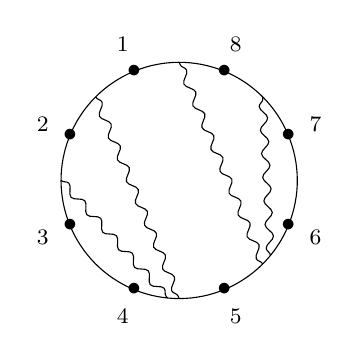
\begin{tikzpicture}[rotate=67.5,baseline=(current bounding box.east)]
	\begin{scope}
	\drawWLD{8}{1.5}
	\drawnumbers
	\drawprop{1}{0}{4}{0}
	\drawprop{2}{0}{4}{-1}
    \drawprop{5}{0}{8}{0}
    \drawprop{5}{1}{7}{0}
		\end{scope}
	\end{tikzpicture}\]

\caption{The Wilson loop diagram $W = \big(\{(1,4), (2,4), (5,7), (5,8)\},[8]\big)$ which has four propagators and eight vertices.}
\label{fig:ex of WLD}
\end{figure}

Let $[n]$ denote the set of integers $\{1,\dots,n\}$ with the obvious cyclic and linear orders.

Generally speaking the propagators in a Wilson loop diagram are undirected, so $(i,j)$ and $(j,i)$ represent the same propagator. If we need to impose a direction on a propagator $p = (i,j)$, for example in order to consider the region ``inside'' or ``outside'' of $p$, we write $(p,<_i)$ to indicate that $p$ is directed from edge $i$ to edge $j$, and $(p,<_j)$ for the opposite direction. 

We also impose the convention that all vertices should always be interpreted in terms of the cyclic order on $V$.  So, for any $i\in V$ we will use $i+1$ to denote the successor of $i$ in $V$.   In particular, if $V = [n]$ then $(n,n+3)$ means the propagator connecting edges $3$ and $n$. This viewpoint is beneficial for us since many of our proofs rely on restricting our attention to a region of the diagram bounded by a given propagator, or to short propagators such as $(i,i+2)$, and these behave the same regardless of whether we cross the ``first'' vertex or not; however, we emphasize that this is different to the standard convention in the physics literature, where propagators are written $(i,j)$ with $1 \leq i<j \leq n$.



\begin{dfn} \label{VPropdfn}
Let $W = (\cP, V)$ be a Wilson loop diagram.
\begin{enumerate}
\item For $p = (i,j) \in \cP$, let $V(p) = \{i, i+1, j, j+1\}$ denote the set of {\bf vertices supporting $p$}. For a set of propagators $P \subseteq \cP$, define 
\[V(P) = \bigcup_{p \in P} V(p)\]
to be the vertex support of $P$.
\item For $U \subseteq V$, the set of {\bf propagators supported on $U$} is denoted by
\[\Prop(U) = \{ p \in \cP\ |\ V(p) \cap U \neq \emptyset \}.\]
Note that a propagator in $\Prop(U)$ does not need to have its entire support contained in $U$. 
\item Vertices of $W$ that do not support any propagators are called {\bf non-supporting}.
\end{enumerate}
\end{dfn}

In particular, we will see in later sections that all four vertices supporting a propagator are important in understanding the contribution of that propagator to the objects represented by the diagram. This motivates the following definition of a subdiagram: any subset $Q$ of the propagators and any subset $U$ of the vertices of $W$ {\em containing the support of $Q$}.

\begin{dfn} \label{subdiagramdfn}
Let $W = (\cP, V)$ be a Wilson loop diagram. Then $W' = (Q,U)$ is a {\bf subdiagram} of $W$ if $Q \subseteq \cP$ and $V(Q) \subseteq U \subseteq V$.
\end{dfn}



With these definitions in hand, we can impose some conditions on the density and behavior of the propagators of Wilson loop diagrams.

\begin{dfn}\label{admisdfn}
A Wilson loop diagram $W = (\cP, V)$ is called {\bf admissible} if:
\begin{enumerate}
\item $|V| \geq |\cP| + 4$.
\item There does not exist a non-empty set of propagators $Q \subseteq \cP$ such that $|V(Q)| < |Q| + 3$.
\item There does not exist a pair of crossing propagators: that is, there does not exist $\{(i,j),(k,l)\} \subseteq \cP$ such that $i < k < j < l$.
\end{enumerate}
 \end{dfn}

The first condition bounds the total number of propagators in the diagram, while the second limits how densely propagators can be fitted into any part of the diagram; in particular, it prohibits propagators that connect two adjacent edges and parallel propagators that start and end on the same pair of edges. The third condition simply requires that propagators are non-crossing. 

These conditions are imposed by the physical interpretation of Wilson loop diagrams (see for example \cite{Adamo:2011pv,Adamo:2012xe,wilsonloop,LipsteinMason}). We therefore restrict our attention in this paper to admissible Wilson loop diagrams and their subdiagrams only. 

Note that a subdiagram $(Q,U)$ of an admissible Wilson loop diagram need not be admissible itself: it inherits conditions 2 and 3 automatically, but we could have $|U| = |Q| + 3$. If a Wilson loop diagrams satisfies conditions 2 and 3 of Definition~\ref{admisdfn}, we call it {\bf weakly admissible}.

These diagrams correspond to (tree level) amplitudes of SYM $N=4$ theory in twistor space. As such, a diagram associates a real value to $n$ particles, one for each vertex. Each particle is represented as a section of a $|\cP|$-vector bundle over twistor space, projected onto a real subspace in a process called bosonization \cite{Arkani-Hamed:2013jha}. In other words, each Wilson loop diagram defines a functional on external particles. This is represented as an integral $I(W)$, which is the equivalent of a Feynman integral in this setting. This integral is comprised of two main components, and interaction matrix, $C(W)$ and a volume form, $\Omega(W)$. These are described below.

A $|\cP| \times n$ matrix $C(W)$ represents the (tree level) particle interactions. Each row of $C(W)$ corresponds to an internal propagator, each column to an external particle. $C(W)$ is defined as follows:

\begin{equation} C(W)_{p,q} = \begin{cases} x_{p,q} & \textrm{ if } q \in V(p) \\
0  & \textrm{ if } q \not \in V(p)  \end{cases}
\;. \label{C(W) dfn}\end{equation} 

The entries $x_{p,q}$ are non-zero real variables. Thus the zero entries in row $p$ correspond to the external particles that the propagator $p$ does not interact with. See Example~\ref{integraldetails} for an example of a diagram $W$ and its associated matrix.

The matrix $C(W)$ defines a positroid cell associated to $W$ in the positive Grassmannian $\Gr(n, |\cP|)$, which we denote by $\Sigma(W)$ \cite{wilsonloop}. Marcott \cite{WLDdim} shows that  the matrix $C(W)$ parametrizes a space whose close is exactly the closure of $\Sigma(W)$. That is, the space defined by $C(W)$ and the cell $\Sigma(W)$ agree up to a set of measure $0$. Most of the work in this paper, and in \cite{generalcombinatoricsI} focuses on characterizing the positroid cell associated to each Wilson loop diagram $W$. 

Note that since there is no ordering on the propagators of $W$, $C(W)$ is only defined up to rearrangement of the rows. When needed, we will impose various orders on these rows. This will not matter, as it does not affect $\Sigma(W)$.

One may also interpret the functional $I(W)$ as associating a volume to each cell $\Sigma(W)$ \cite{wilsonloop, Amplituhedronsquared, HeslopStewart}. The volume form is written in terms of the elements of $C(W)$ as  \begin{equation} \label{eq:omega(W) def}\Omega(W) = \frac{\prod_{r=1}^{|\cP|} \prod_{v \in V(p_r)} \textrm{d}x_{p_r}}{R(W)} \;, \end{equation}
where the denominator $R(W)$ is given in Definition~\ref{def R(W)} below. The interested reader is referred to \cite{Adamo:2012xe,HeslopStewart,LipsteinMason} for more information about the volume form. 

For a fixed number of propagators and particles, the tree level amplitude of the Wilson loop diagrams is computed as the sum of the $I(W)$ for all $W$ of the correct size. By \cite{Adamo:2011pv,Adamo:2012xe,Arkani-Hamed:2013jha} this sum is finite for all sets of external particles, i.e. we have 
\bas \mathcal{A}_{k, n}^{tree} = \sum_{\substack{W = (\cP, [n]), \\ |\cP| = k}} I(W) <\infty. \eas

In particular, this implies that any singularities in the integrals $I(W)$ must cancel out in the sum, in particular, all poles arising from $R(W)$ must cancel. Specifically, these poles must cancel on the boundaries of the positroid cells $\Sigma(W)$, analogous to the analysis in \cite{Arkani-Hamed:2013jha}. This has been checked for particular classes of examples (e.g. \cite{casestudy, Amplituhedronsquared, HeslopStewart}) but has not been proven in general.

With this motivation in mind, in this paper we study the denominator $R(W)$ of the volume form $\Omega(W)$, which we define next.

\begin{dfn}\label{def R(W)}
Let $W = (\cP,V)$ be an admissible Wilson loop diagram, and fix an edge $e$. Let $\{p_1 \ldots p_r\}$ be the propagators with one end lying on edge $e$ under a counterclockwise ordering. That is, $p_1$ is closest to the vertex $e$, $p_i$ is positioned counterclockwise to $p_{i+1}$ and $p_r$ is the clockwise most propagator on this edge (closest to vertex $e+1$). Define the polynomial
\[ R_e =  x_{p_1,e+1} \prod_{j= 1}^{r-1} \left((x_{p_j,e} x_{p_{j+1},e+1} - x_{p_{j+1},e} x_{p_{j},e+1} ) \right) x_{p_r,e}\;\]
to be the component of $R(W)$ associated to edge $e$. Note that if $r = 1$ (i.e. there is exactly one propagator lying on edge $e$) then this expression simplifies to $R_e = x_{p,e} x_{p,e+1}$. If $r=0$, set $R_e = 1$. The denominator $R(W)$ is defined to be the product of all of the $R_e$, i.e. 
\[R(W) = \prod_{e \in V} R_e.\]
\end{dfn}

In Section \ref{sec poles}, we show that the denominator $R(W)$ is determined by the positroid cell $\Sigma(W)$ and the structure of $W$, as encapsulated by $C(W)$. In fact, it can be read directly off of $C(W)$, in terms of a characterization of $\Sigma(W)$ called the Grassmann necklace (see Definition~\ref{def:grassmann necklace}) as shown in Algorithm \ref{alg:put GN on WLD}. We also give an algorithm to read $R(W)$ directly from the Wilson loop diagram, paving the way for a general study of these poles in future. 

We end this section with an example of computing $C(W)$ and $R(W)$ for a particular Wilson loop diagram $W$.

\begin{eg} \label{integraldetails}
Consider the admissible Wilson loop diagram 
\[W = \big(\{(1,4), (2,4), (5,7), (5,8)\},[8]\big),\]
from Figure~\ref{fig:ex of WLD}. Ordering the propagators as listed above, we obtain the associated matrix
\[ C(W) = \left(
\begin{array}{cccccccc}
x_{1,1} & x_{1,2} & 0 & x_{1,4} & x_{1,5} & 0 & 0 & 0 \\
0 & x_{2,2} & x_{2,3} & x_{2,4} & x_{2,5} & 0 & 0 & 0 \\
0 & 0 & 0 & 0 & x_{3,5} & x_{3,6} & x_{3,7} & x_{3,8} \\
x_{4,1} & 0 & 0 & 0 & x_{4,5} & x_{4,6} & 0 & x_{4,8}  \\
\end{array}
\right) \;.\]

To calculate $R(W)$, we first compute the polynomials associated to each edge of $W$: \bmls R_1 = x_{1,1} x_{1, 2}\quad R_2 = x_{2,2} x_{2,3} \quad R_4 = x_{2,5} (x_{2,4}x_{1,5} - x_{2,5}x_{1,4})x_{1,4} \\ R_5 = x_{4,6} (x_{4,5}x_{3,6} - x_{3,5}x_{4,6})x_{3,5} \quad R_7 = x_{3,7} x_{3,8} \quad R_8 = x_{4,8} x_{4,1} \;.\emls All other $R_e$ are $1$.  Finally, the integrand associated to this Wilson loop diagram (recall equation~\eqref{eq:omega(W) def}) is \bas \Omega(W) = \frac{\textrm{d}x_{1,1}\textrm{d}x_{1,2}\textrm{d}x_{1,4}\textrm{d}x_{1,5}\textrm{d}x_{2,2}\textrm{d}x_{2,3}\textrm{d}x_{2,4}\textrm{d}x_{2,5}\textrm{d}x_{3,5}\textrm{d}x_{3,6}\textrm{d}x_{3,7}\textrm{d}x_{3,8}\textrm{d}x_{4,5}\textrm{d}x_{4,6}\textrm{d}x_{4,8}\textrm{d}x_{4,1}}{x_{1,1} x_{1, 2}x_{2,2} x_{2,3}x_{2,5} (x_{2,4}x_{1,5} - x_{2,5}x_{1,4})x_{1,4}x_{4,6} (x_{4,5}x_{3,6} - x_{3,5}x_{4,6})x_{3,5}x_{3,7} x_{3,8}x_{4,8} x_{4,1}} \;. \eas
\end{eg}


\subsection{Positroids, Grassmann necklaces, and Le diagrams}\label{sec:positroid background}

We summarize here only the subset of positroid theory that we require in this paper; the interested reader is referred to \cite{Postnikov} for more details. 

Let $\binom{[n]}{k}$ denote the set of all $k$-subsets of $[n]$.  

For our purposes, a {\bf positroid} is\footnote{Note that matroid isomorphism allows arbitrary permutations of the ground set but positroid isomorphism allows only cyclic permutations, so the property of being a positroid is not in general preserved by matroid isomorphism.} a matroid $M$ (with ground set $[n]$ and bases $\cB \subseteq \binom{[n]}{k}$) which can be represented by an element of the positive Grassmannian $\Gr(k,n)$. In other words, there exists a full-rank $k\times n$ real matrix whose $k\times k$ minors are all nonnegative and such that the minor given by the columns of $J$ 
is positive if and only if $J \in \cB$.

Postnikov shows in \cite{Postnikov} that the positroids of $\Gr(k,n)$ are indexed by many different collections of objects, each with their own advantages and disadvantages. The two most suited to our purposes are Grassmann necklaces and Le diagrams, which we introduce below. In order to do so, we first need some preliminary definitions.

For each $j \in [n]$, we can define a total order $<_j$ on the interval $[n]$ by
\[ j <_j j+1 <_j \dots <_j n <_j 1 \dots <_j j-1\;.\]
This in turn induces a total order on $\binom{[n]}{k}$, namely the lexicographic order with respect to $<_j$.  It also induces a separate partial order $\gale{j}$ on $\binom{[n]}{k}$ (the {\bf Gale order} \cite{Gale}), which is defined as follows: for 
\[A = \{a_1 <_j a_2 <_j \dots <_j a_k\} \text{ and } B = \{b_1 <_j b_2 <_j \dots <_j b_k\} \in \binom{[n]}{k},\] we define
\[A \gale{j} B \text{ if and only if } a_r \leq_j b_r \text{ for all }1 \leq r \leq k.\]
For example, in $\binom{[6]}{3}$ we have $\{2,5,6\}\gale{2} \{2,6,1\}$ but $\{2,5,6\}\not\gale{2}\{3,4,6\}$.


\begin{dfn}\label{def:grassmann necklace}
A {\bf Grassmann necklace} of type $(k,n)$ is a sequence $(I_1, \dots, I_n)$ of $n$ sets $I_i \in \binom{[n]}{k}$ such that for each $i \in [n]$:
\begin{itemize}
\item if $i \in I_i$, then $I_{i+1} = \big(I_i \backslash \{i\}\big) \cup \{j\}$ for some $j \in[n]$.
\item if $i \not\in I_i$, then $I_{i+1} = I_i$.
\end{itemize}
By convention, we set $I_{n+1} = I_1$.
\end{dfn}

By \cite[Theorem 17.1]{Postnikov}, the Grassmann necklaces of type $(k,n)$ are in 1-1 correspondence with the positroid cells in $\Gr(k,n)$. Each term $I_i$ is simply the minimal (with respect to the $<_i$-lex order) basis of the positroid. A characterization of all bases of the positroid in terms of the Grassmann necklace and the Gale order was given by Oh in \cite[Theorem 8]{Oh}: if $(I_1, \dots, I_n)$ is the Grassmann necklace associated to a positroid $M = ([n],\cB)$, then the bases of $M$ are exactly
\ba \cB = \left\{J \in \binom{[n]}{k}\ \Big|\ I_i \gale{i} J \ \ \forall i \in [n]\right\}. \label{basesofmatroids}\ea
Thus the Grassmann necklace is well suited to testing whether a given $k$-set is a basis for $M$, and for generating a list of all bases of $M$.


\begin{dfn}\label{def:le diagram}
A {\bf Le diagram} is a Young diagram in which every square contains either a $+$ or a $0$, subject to the rule that if a square contains a $0$ then either all squares to its left (in the same row) must also contain a $0$, or all squares above it (in the same column) must also contain a $0$, or both.
\end{dfn}

By \cite[Theorem 6.5]{Postnikov}, the set of all Le diagrams that fit within a $k\times(n-k)$ rectangle is in 1-1 correspondence with the positroid cells of $\Gr(k,n)$. Le diagrams are particularly useful for comparing dimensions of positroids, since the dimension of a positroid is equal to the number of $+$ squares in its Le diagram \cite[Theorem 6.5]{Postnikov}.

The rows and columns of a Le diagram are labelled as follows: given a Le diagram fitting inside a $k\times (n-k)$ box, arrange the numbers $1,2, \dots, n$ along its southeast border, starting from the top-right corner. See Figure \ref{fig:row column numbering} for examples.

\begin{figure}[h!]
\[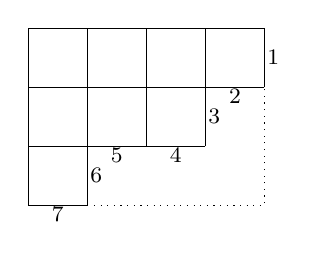
\begin{tikzpicture}[baseline=(current bounding box.east),scale=0.75]
\draw (1,0) grid (2,3);
\draw (2,1) grid (4,3);
\draw (4,2) grid (5,3);
\draw[dotted] (2,0) -- (5,0) -- (5,2);

\node at (5.15,2.5) {\footnotesize$1$};
\node at (4.5,1.85) {\footnotesize$2$};
\node at (4.15,1.5) {\footnotesize$3$};
\node at (3.5,0.85) {\footnotesize$4$};
\node at (2.5,0.85) {\footnotesize$5$};
\node at (2.15,0.5) {\footnotesize$6$};
\node at (1.5,-0.15) {\footnotesize$7$};
%\node at (0.5,-0.15) {\footnotesize$8$};
\end{tikzpicture}
\qquad \qquad
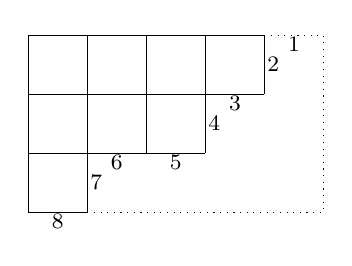
\begin{tikzpicture}[baseline=(current bounding box.east),scale=0.75]
\draw (1,0) grid (2,3);
\draw (2,1) grid (4,3);
\draw (4,2) grid (5,3);
\draw[dotted] (2,0) -- (6,0) -- (6,3) -- (5,3);

\node at (5.5,2.85) {\footnotesize$1$};
\node at (5.15,2.5) {\footnotesize$2$};
\node at (4.5,1.85) {\footnotesize$3$};
\node at (4.15,1.5) {\footnotesize$4$};
\node at (3.5,0.85) {\footnotesize$5$};
\node at (2.5,0.85) {\footnotesize$6$};
\node at (2.15,0.5) {\footnotesize$7$};
\node at (1.5,-0.15) {\footnotesize$8$};
%\node at (0.5,-0.15) {\footnotesize$9$};
\end{tikzpicture}
\]
\caption{Row and column numbering for a Young diagram with $k = 3$, $n = 7$ (left) and $k = 3$, $n = 8$ (right). The top left box has coordinates $(1,7)$ in the left diagram, and $(2,8)$ in the right diagram.}
\label{fig:row column numbering}
\end{figure}

Specifying a $k$-subset $J \subseteq [n]$ therefore uniquely determines the shape of the Le diagram, by taking the elements of $J$ to be the row indices of the diagram.

An algorithm for constructing the Le diagram associated to a Grassmann necklace was given by Agarwala and Fryer in \cite{reversingOh}. Since we will make use of this algorithm in Section~\ref{sec dim} below, we summarize the process here.
\begin{algorithm}\label{alg:GN to Le} \ \cite[Algorithm 2]{reversingOh}
Let $(I_1,\dots,I_n)$ be a Grassmann necklace of type $(k,n)$. Within a $k \times(n-k)$ square, draw the Young diagram whose rows are labelled by $I_1$ (as per the convention above).

For each $i$, $2 \leq i \leq n$:
\begin{itemize}
\item Write \[I_1 \setminus I_i = \{a_1 > a_2 > \dots > a_r\}, \quad I_i \setminus I_1 = \{b_1 < b_2 < \dots < b_r\},\]
where the inequalities denote the $<_1$ order (subscripts suppressed for clarity).
\item For $1 \leq j \leq r$ , place a $+$ in square $(a_j,b_j)$ of the diagram. (We will sometimes refer to this $+$ as being {\em in the $a_j \rightarrow b_j$ position}.)
\end{itemize}
After performing the above for $2 \leq i \leq n$, place a $0$ in any remaining unfilled boxes.
\end{algorithm}

An algorithm for constructing the Grassmann necklace of a Le diagram also exists; this was given by Oh in \cite{Oh}. A method for using the Le diagram to test whether a given $k$-subset is a basis for the corresponding positroid or not was given by Casteels in \cite{CasteelsPaths}.



\subsection{Wilson loop diagrams as positroids}\label{sec:WLD as positroids}


Let $W = (\cP,[n])$ be an admissible Wilson loop diagram with $k$ propagators, and $C(W)$ the associated matrix defined in equation~\eqref{C(W) dfn}. Let $M(W)$ be the matroid realized by $C(W)$, i.e. the matroid with ground set $[n]$ whose independent sets are exactly the sets $V \subseteq [n]$ such that the columns of $C(W)$ indexed by $V$ are linearly independent.

In \cite{wilsonloop}, Agarwala and Marin-Amat show that $M(W)$ can also be read directly from the Wilson loop diagram itself:

\begin{thm} \label{thm WLD defines matroid} \cite[Theorem 3.6]{wilsonloop} The independent sets of the matroid $M(W)$ associated to an admissible Wilson loop diagram $W = (\cP,[n])$ and realized by $C(W)$ are exactly those subsets $V \subseteq [n]$ such that $\nexists U\subseteq V$ satisfying $|\Prop(U)| < |U|$. \end{thm}
In other words, the independent sets of $M(W)$ correspond to sets of vertices in $W$ in which no subset supports fewer propagators than the vertices it contains.

One useful corollary of this, which we will want to keep in mind later, is the following.
\begin{cor}\label{lem basis as perm}
Let $W = (\cP,[n])$ be an admissible Wilson loop diagram and let $M(W)$ be its associated matroid. A subset $J \subseteq [n]$ is an independent set of $M(W)$ if and only if there exists an injective set map $f : J \rightarrow \cP$ with the property that for each $j\in J$ we have $j \in V(f(j))$.
\end{cor}

\begin{proof}
  This follows as a corollary of the previous theorem by induction in one direction and the pigeonhole principle in the other direction.  

  Alternatively we can simply think about the condition of linear independence in the matrix $C(W)$, the corollary can also be proved directly by linear algebra and the definition of $C(W)$ as follows.

  Because the nonzero entries of $C(W)$ are independent indeterminants, $J$ is an independent set if and only if there is some choice of $|J|$ nonzero entries of $C(W)$ one in each row associated to an element of $J$ and each in different columns. Each entry in $C(W)$ identifies a propagator by the row of the entry and a vertex by the column of the entry.  The entry is nonzero if and only if the propagator is supported on that vertex.  Consequently, a choice of $|J|$ nonzero entries of $C(W)$ one in each row associated to an element of $J$ and each in different columns is equivalent to an assignment of the propagators of $J$ to supporting vertices so that no two are assigned to the same vertex.  Such an assignment of the propagators of $J$ to supporting vertices is exactly a map $f$ as described in the statment, hence proving the result.
\end{proof}

In particular, this corollary says that a subset $J$ of $[n]$ is a basis of $M(W)$ if and only if there is a set bijection between $J$ and $\cP$ with the property that for each $j\in J$ the propagator associated to $j$ under the bijection is supported on vertex $j$.


By relating the behavior of the propagators in $W$ to the matroidal properties of $M(W)$, Agarwala and Marin-Amat also showed that $M(W)$ is in fact a positroid whenever $W$ is admissible \cite[Corollary 3.39]{wilsonloop}.

However, to go from the Wilson loop diagram $W$ to the positroid cell, one had to go through the matroid explicitly realized via $C(W)$, then make a list of all its non-zero $k\times k$ minors and extract the Le diagram or Grassmann necklace via the methods described in Section~\ref{sec:positroid background}. In \cite{casestudy}, Agarwala and Fryer apply this process in the smallest non-trivial case: admissible Wilson loop diagrams with two propagators on six vertices. Even in this simple case, we see that the mapping from admissible WLD to positroid cells is neither one-to-one nor onto, and the process described above makes it almost impossible to track the relationship between the original Wilson loop diagram and the resulting positroid.

Our first goal is therefore to find a better method of obtaining the positroid associated to a given Wilson loop diagram; this is the focus of the next section.

\begin{rmk}
While this paper primarily approaches proofs from a combinatorial point of view, readers with a background in matroid theory are encouraged to keep the matroidal viewpoint in mind throughout; we expect that the two approaches will be complementary and will build upon each other. See \cite{generalcombinatoricsI} for some related results concerning the positroids of Wilson loop diagrams obtained by viewing them primarily as matroids.
\end{rmk}




\section{Wilson Loop diagrams and their Grassmann necklaces}\label{sec GN algorithm}



In this section we will give an algorithm (Algorithm~\ref{alg:put GN on WLD}) to go directly from a Wilson loop diagram to the Grassmann necklace of its positroid. This is a useful result in and of itself, as it greatly simplifies the process of identifying the positroid associated to a given Wilson loop diagram. Furthemore, we use it to characterize loops and coloops in the positroid associated to a Wilson loop diagram (Corrollary \ref{no coloops}). It allows us to see how the Le diagram assoicated to a Wilson loop diagram changes as one adds propagators in certain positions (Theorem \ref{thm dim}). Indeed, the techniques we develop in this section to verify that our algorithm produces the correct Grassmann necklace will also be used repeatedly in later sections to calculate the dimension of the associated positroid cell (section \ref{sec dim}) and to study the structure of the poles of the associated integral $I(W)$ (section \ref{sec poles}).

One of the key insights is that each element of the Grassmann necklace can be viewed as a function from the propagators of the diagram to the vertices in the Grassman necklace element.  This is captured in Definition~\ref{def I_i as a function}, and used throughout the paper.

%\note{Sian thinks that a section roadmap here would be overkill: we gave a roadmap in section 1, each subsection has its own little intro roadmap, and I've added a ref to the algorithm above so that people can skip straight to it if they want}

%In Section~\ref{sec:propagator configs} we examine the structure of admissible Wilson loop diagrams and prove several technical lemmas about configurations of propagators appearing in these diagrams. In Section~\ref{sec:GN alg} we state the algorithm that extracts the Grassmann necklace of a given diagram (see Algorithm~\ref{alg:put GN on WLD}) and 

Throughout this section, $W = (\cP,[n])$ is an admissible Wilson loop diagram with $k$ propagators.





\subsection{Propagator configurations in admissible Wilson loop diagrams}\label{sec:propagator configs}

Before we can describe the algorithm for extracting the Grassmann necklace of $M(W)$ from the Wilson loop diagram $W$, we require some initial results about the behavior of propagators in admissible WLD.



\begin{dfn}\label{props inside p}
Let $W = (\cP, [n])$ be a weakly admissible Wilson loop diagram, with $p \in \cP$ supported on edges $i$ and $j$. Write $(p, <_i)$ to represent the same propagator directed from $i$ to $j$. Then the sets of propagators {\bf inside} and {\bf outside} of $(p,<_i)$ are defined to be
\begin{gather*}\cP_{in}(p,<_i) = \{ (k,l) \in \cP \ |\ i \leq_i k <_i l \leq_i j \}, \\
\cP_{out}(p,<_i) = \cP\setminus \cP_{in}(p,<_i),
\end{gather*}
respectively.
\end{dfn}
Note that we have $p\in \cP_{in}(p, <_i)$ and so $\cP_{in}(p, <_i) = \cP_{out}(p, <_j)\cup\{p\}$.


\begin{eg}
Let $W$ be the Wilson loop diagram from Figure \ref{fig:ex of WLD}, reproduced here for convenience.  \[W\ =\ 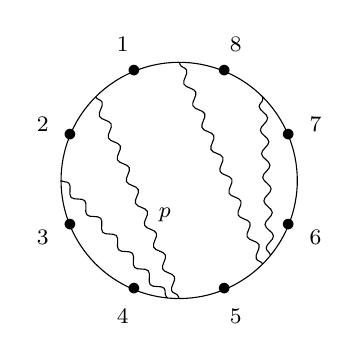
\begin{tikzpicture}[rotate=67.5,baseline=(current bounding box.east)]
	\begin{scope}
	\drawWLD{8}{1.5}
	\drawnumbers
	\drawlabeledprop{1}{0}{4}{0}{\footnotesize \qquad \ $p$}
	\drawprop{2}{0}{4}{-1}
    \drawprop{5}{0}{8}{0}
    \drawprop{5}{1}{7}{0}
		\end{scope}
	\end{tikzpicture}\]

Let $p$ be the propatagor $p = (1, 4)$. Then $\cP_{in}(p, <_4) = \{(1,4), (5, 8), (5, 7) \}$ and $\cP_{out}(p, <_4) = \{(2,4) \}$
\end{eg}

\begin{dfn}
Let $p = (i,j) \in \cP$ be a propagator in $W$.  Define the {\bf length} of $p$ to be 
\[\ell(p) \  =\ \min\big\{|[i+1,j]|,|[j+1,i]|\big\}.\]
\end{dfn}
In other words, $\ell(p)$ is the size of the smaller of the sets of vertices on either side of the propagator $p$.


\begin{rmk}\label{rem:props of length 2 and 3} 
  The following observations about configurations of propagators of short length in a weakly admissibly Wilson loop diagram $W$ are easily verified:
 \begin{enumerate}
\item If $p = (i,i+3)$ is a propagator of length 3, then the middle vertex $i+2$ supports at most one propagator.
\item If every vertex in $W$ supports at least one propagator, then $W$ admits at least one propagator of length 2.  Furthermore, by the same reasoning, if $p=(i,j)$ is a propagator of $W$ and every vertex in $[i,j]$ supports at least one propagator then there is at least one propagator of length $2$ in $\mathcal{P}_{in}(p, <_i)$.
\end{enumerate}
\end{rmk}



\begin{figure}[h]
\[
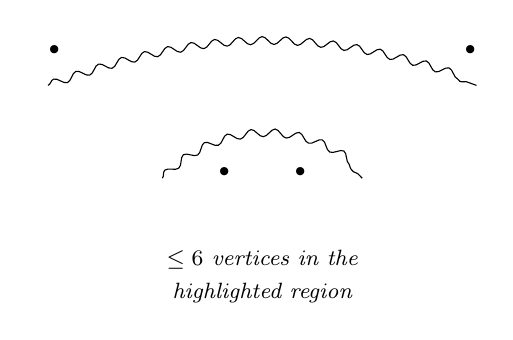
\begin{tikzpicture}[baseline=(current bounding box.north)]
  \begin{scope}
  \drawWLDfragment[7]{3}{0.4} 
  %\drawnumberspartial % use this to debug
  \centerarc[linehighlight](0,0)(\zero + 1.43*\step:\zero+6.6*\step:\radius)
  \newnode{1}{}
  \newnode{3.55}{}
  \newnode{4.45}{}
  \newnode{7}{}
    \begin{scope}
    \clipcenterarc(0,0)(\startpoint:\endpoint:\radius)
  \newpropbend{1.3}{6.7}{20}
  \newpropbend{2.9}{5.1}{45}
  \end{scope}
  \node[align=center] at (\zero + 4*\step:\radius*1.43) {\footnotesize \em $\leq 6$ vertices in the \\ \footnotesize \em highlighted region};
\end{scope}
\end{tikzpicture}
\qquad \qquad \qquad
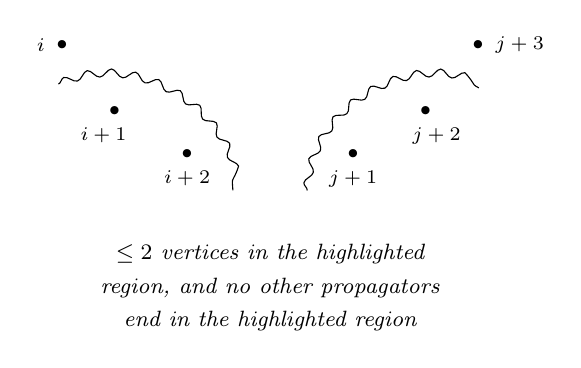
\begin{tikzpicture}[baseline=(current bounding box.north)]
  \begin{scope}
  \drawWLDfragment[7]{3}{0.4} 
  %\drawnumberspartial % use this to debug
  \centerarc[linehighlight](0,0)(\zero + 3.67*\step:\zero+4.43*\step:\radius)
  \newnode{1}{i}
  \newnode[below]{2}{i+1\ \ \ }
  \newnode[below]{3}{i+2}
  \newnode[below]{5}{j+1}
  \newnode[below]{6}{\quad j+2}
  \newnode[right]{7}{j+3}
      \begin{scope}
    \clipcenterarc(0,0)(\startpoint:\endpoint:\radius)
  \newpropbend{1.35}{3.6}{55}
  \newpropbend{4.4}{6.6}{55}
  \end{scope}
  \node[align=center] at (\zero + 4*\step:\radius*1.5) {\footnotesize \em $\leq 2$ vertices in the highlighted \\ \footnotesize \em region, and  no other propagators \\ \em \footnotesize end in the highlighted region};
\end{scope}
\end{tikzpicture}
\]
\caption{The two configurations described in Lemma~\ref{lem sian}; every weakly admissible Wilson loop diagram with no non-supporting vertices supports at least one example of at least one of these configurations.}\label{fig: small configs}
\end{figure}


The following lemma establishes certain configurations of propagators that must exist in any admissible diagram with no non-supporting vertices. We make use of this result in several induction proofs below. 

\begin{lem}\label{lem sian}
  Let $W$ be a weakly admissible WLD with at least 5 vertices and in which each vertex supports at least one propagator.  Then at least one of the following two things occurs:
  \begin{enumerate}
    \item $W$ has a propagator of length $\leq 6$ with a propagator of length 2 on one side of it and nothing else on that side.\label{item big and 2}
    \item There exists a pair of propagators of length $2$ with the property that the first propagator is $(i, i+2)$, the second is $(j, j+2)$, no other propagator ends between vertices $i+2$ and $j+1$, and $j\in\{i+2, i+3, i+4\}$.\label{item pair of 2s}
  \end{enumerate}
See Figure~\ref{fig: small configs} for an illustration of the two configurations.
\end{lem}

\begin{proof}
Suppose first that $W$ has a propagator of length $3$, say $p=(i, i+3)$.  By Remark~\ref{rem:props of length 2 and 3} and the fact that every vertex of $W$ supports at least one propagator, we have that $i+2$ supports exactly one propagator and this propagator must have length 2 by noncrossingness.  This gives us an instance of configuration~\ref{item big and 2} from the statement.

Now suppose $W$ has no propagators of length $3$.
  
We will inductively construct a sequence of propagators $p_r$ and $q_r$, with $\ell(p_r) = 2$ for each $r$ and such that either:
\begin{itemize}
\item $p_r$ forms part of configuration \ref{item big and 2} or \ref{item pair of 2s} from the statement, at which point the induction terminates, 
  %a configuration \eqref{eq:2 prop config} in $D$
{\em or} 
\item there is a propagator $q_r$ satisfying $\ell(q_r) \geq 4$, and $\{p_1, \ldots, p_r, q_1, \ldots, q_{r-1}\}$ are all on the same side of $q_r$.  
\end{itemize}

\begin{figure}
\[
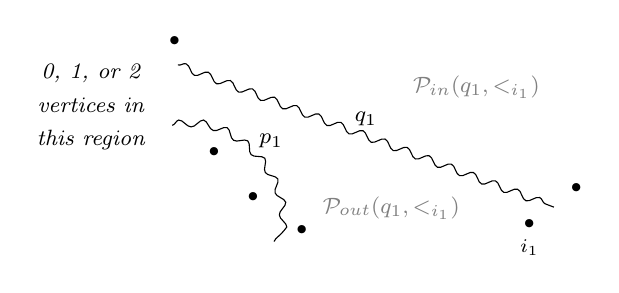
\begin{tikzpicture}[baseline=(current bounding box.east),rotate=-20]
	\begin{scope}
	\drawWLDfragment[10]{3}{0.4} 
	%\drawnumberspartial % use this to debug
	\centerarc[linehighlight](0,0)(\zero + 1.5*\step:\zero + 2.35*\step:\radius)
	\newnode{1}{}
	\newnode{3}{}
	\newnode{4}{}
	\newnode{5}{}
	\newnode[below]{9}{i_1}
	\newnode{10}{}
	\newprop[midway,above]{1.4}{9.5}{\footnotesize $q_1$}
	\begin{scope}
		\clipcenterarc(0,0)(\startpoint:\endpoint:\radius)
		\newpropbend{2.3}{4.7}{60}
		\node at (\zero + 3.5*\step:\radius*0.78) {\footnotesize $p_1$};
	\end{scope}
\node[align = center] at (\zero +1.7*\step:\radius*1.4) {\footnotesize \em 0, 1, or 2 \\ \footnotesize \em vertices in \\ \footnotesize \em this region};
\node[gray] at (\zero + 10*\step:\radius*0.4) {\footnotesize$\cP_{in}(q_1,<_{i_1})$};
\node[gray] at (\zero + 6.5*\step:\radius*0.8) {\footnotesize $\cP_{out}(q_1,<_{i_1})$};
\end{scope}
\end{tikzpicture}
\]
\caption{The base case of the induction in Lemma~\ref{lem sian}.}\label{fig base case lem sian} \end{figure}

We can then choose the orientation of $q_r$ so that the previous $p_i$ and $q_i$ are all on the outside of $q_r$, and restrict our attention to the subdiagram $(\cP_{in}(q_r),[n])$. By the finiteness of $W$ this must eventually terminate in one of the desired configurations. %a configuration of the form \eqref{eq:2 prop config}.

Start by choosing a propagator $p_1 = (j_1,j_1+2)$ of length 2 in $W$ (which exists by Remark~\ref{rem:props of length 2 and 3}).  If it is part of one of the configurations we are looking for then we are done, 
%a configuration \eqref{eq:2 prop config} we are done,
so suppose otherwise. 

From our existing assumptions, we know the following facts: $p_1$ is not in configuration \ref{item pair of 2s}, there are no propagators of length $3$, and every vertex supports at least one propagator.  Therefore there must be a propagator of length $\geq 4$ with one end on edge $j_1$ or on edge $j_1-1$ or on edge $j_1-2$.  Let $q_1 = (i_1, k_1)$ be this propagator, oriented such that $p_1 \in \cP_{out}(q_1,<_{i_1})$; see Figure~\ref{fig base case lem sian}. This completes the base case.

Now suppose $q_{r} = (i_r, k_r)$ exists by the induction hypothesis and is oriented $(q_r, <_{i_r})$ so that the previous $p_i$ and $q_i$ are on the outside. For the rest of this proof, we assume this orientation and drop the $<_{i_r}$ from the notation.

Let $W_r := (\cP_{in}(q_r),[n])$ be the subdiagram of $W$ consisting only of those propagators inside $q_r$ (including $q_r$ itself); in particular $W_r$ contains none of the previous $p_i$ or $q_i$. By the original hypotheses on $W$, every vertex in $[i_r,k_{r+1}]$ (of which there are at least 4, since $\ell(q_r) \geq 4$) must support at least one propagator. Therefore $W_r$ admits at least one propagator of length 2 (by Remark~\ref{rem:props of length 2 and 3}) and no propagators of length $3$ (by our assumption on $W$).

Let $p_{r+1} = (j_{r+1}, j_{r+1}+2)$ be a propagator of length 2 in $W_r$; if it forms part of configuration \ref{item big and 2} or \ref{item pair of 2s}
%the configuration \eqref{eq:2 prop config}
then we are done, so assume otherwise. 

Note that we could replace $q_r$ by another propagator $q'_{r}$ in $W_r = (\cP_{in}(q_r), [n])$, as long as $p_{r+1}$ and $q_r$ are on opposite sides of $q_r'$: such a new $q'_{r}$ would still satisfy all of the induction hypotheses. (See Figure~\ref{fig smallest q in lem sian}.) Therefore without loss of generality we may assume that $\cP_{in}(q_r)$ does not contain any propagators (other than $q_r$ itself) which satisfy the induction hypotheses, i.e. we assume that there are no other propagators with $p_{r+1}$ on one side and $q_r$ on the other.

\begin{figure}[h]
\vspace{1cm}
\[
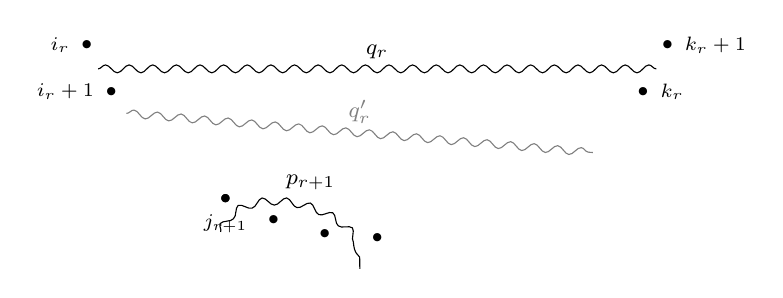
\begin{tikzpicture}[baseline=(current bounding box.east)]
	\begin{scope}
	\drawWLDfragment[15]{4}{0.4} 
	%\drawnumberspartial % use this to debug
	\newnode[left]{1}{i_r}
	\newnode[left]{2}{i_r+1}
	\newnode{5}{}
	\newnode{6}{}
	\newnode{7}{}
	\newnode{8}{}
	\newnode[right]{14}{k_r}
	\newnode[right]{15}{k_r+1}
	\newnode[below]{5}{j_{r+1}}
	\newprop[midway,above]{1.5}{14.5}{\footnotesize $q_r$}
	\draw[smallpropagator,gray] (\zero+2.5*\step:\radius) -- (\zero + 12.5*\step:\radius) node[midway,above,gray] {\footnotesize $q_{r}'$};
	\begin{scope}
		\clipcenterarc(0,0)(\startpoint:\endpoint:\radius)
		\newpropbend{5.2}{7.7}{80}
		\node at (\zero + 6.5*\step:\radius*0.85) {\footnotesize $p_{r+1}$};
	\end{scope}
\end{scope}
\end{tikzpicture}
\]
\caption{We can replace $q_r$ with $q'_r$ as long as $q_r$ and $p_{r+1}$ are on opposite sides of $q'_r$.}
\label{fig smallest q in lem sian}
\end{figure}

There are two cases to consider.

The first case is that $i_r \leq j_{r+1} \leq i_r+2$ and $k_r-2 \leq j_{r+1}+2 \leq k_{r}$ (so $p_{r+1}$ has one end before $i_{r} + 3$ and the other after $k_{r} - 2$, i.e. there are at most two vertices between an endpoint of $p_{r+1}$ and an endpoint of $q_r$).  Then since $p_{r+1}$ has length 2, it must be that $(i_r+3)+1 \geq k_r-2$ and so $q_r$ has length $\leq 6$.  By the minimality assumption on $q_r$, no propagator in $W_r$ has $q_r$ on one side and $p_{r+1}$ on the other side. Therefore, any propagator in $W_r$ other than $q_r$ and $p_{r+1}$ must be of the form $(i,j)$ with $i_r\leq i < j\leq i_r+2$ or $k_r-2 \leq i < j\leq k_r$. Both of these require that $(i,j)$ has length 2, and so we have configuration \ref{item pair of 2s} which we have already assumed does not occur.  Consequently, $W_r$ contains only the two propagators $q_r$ and $p_{r+1}$, yielding configuration \ref{item big and 2} from the lemma statement and again contradicting our assumption. Therefore this first case cannot occur.

The second case is that there are at least $3$ vertices between one endpoint of $p_{r+1}$ and the nearest endpoint of $q_r$. In other words, (at least) one of the following four things happen:
\begin{itemize} 
\item $i_r+3 \leq j_{r+1}\leq k_r-3$ (one endpoint of $p_{r+1}$ has at least 3 vertices between it and the nearest enpoint of $q_r$), or
\item $i_r+3 \leq j_{r+1}+2\leq k_r-3$ (one endpoint of $p_{r+1}$ has at least 3 vertices between it and the nearest enpoint of $q_r$), or
\item $i_r = j_{r+1}$ ($p_{r+1}$ and $q_r$ share an end edge), or 
\item $k_r = j_{r+1} +2$  ($p_{r+1}$ and $q_r$ share an end edge)
\end{itemize}
In other words, at least one end of $p_{r+1}$ is supported entirely by vertices in the interval $[i_r+3,k_r+2]$ (the first two bullet points) or both ends lie in $[i_r, i_r+3]$ (third point) or both ends lie in $[k_r-2, k_r+1]$ (fourth point). These situations all behave similarly, and by symmetry it suffices to only consider the second and third possibilities. 

Since there are at least $3$ vertices between one endpoint of $p_{r+1}$ and the nearest endpoint of $q_r$,  $j_{r+1}+4 \leq k_r-1$ in both of these situations, the vertex $j_{r+1}+4$ is in $[i_r, k_r+1]$ but does not support either $q_r$ or $p_{r+1}$, and must therefore support some other propagator $t$.  Since $p_{r+1}$ is not part of configuration \ref{item pair of 2s} and $W_r$ has no propagators of length 3, it follows that $\ell(t) \geq 4$.  If $q_r$ and $p_{r+1}$ were on different sides of $t$ then this would contradict the minimality of $q_r$.  Therefore we can orient $t$ so that all previous $q_i$ and $p_i$ belong to $\cP_{out}(t)$, and set $q_{r+1} = t$ to continue the induction.

The overall result then follows by induction.

\end{proof}


\begin{rmk}
In the case that all vertices of an admissible WLD $W$ support at least two propagators, then Lemma~\ref{lem sian} substantially simplifies.  By Remark~\ref{rem:props of length 2 and 3}, $W$ has no propagators of length $3$.  Configuration \ref{item big and 2} necessarily entails vertices with support $1$ as does configuration \ref{item pair of 2s} unless $j=i+2$.  So in the case that $W$ has all vertices with support at least two then $W$ must contain a pair of propagators of length $2$  with the property that the first propagator is $(i, i+2)$, the second is $(i+2, i+4)$ and no other propagator ends on the edge $i+2$.
\end{rmk}


\subsection{From Wilson Loop diagrams to Grassmann Necklaces}\label{sec:GN alg}

In this section, we give an algorithm for passing directly from the Wilson loop diagrams to its Grassmann necklace. This not only greatly simplifies the previously known process to obtain a positroid cell from a Wilson loop diagram, but will also allow us to relate the behavior of the positroid $M(W)$ directly to the configuration of progators in $W$. In section \ref{sec poles} we see that the denominator, $R(W)$, of the integrand associated to a Wilson loop diagram, $I(W)$, can be written in terms of the Grassman Necklace of a diagram. 

The fact that Algorithm~\ref{alg:put GN on WLD} does construct the required Grassmann necklace is proved in Theorem~\ref{res:alg gives GN}. A worked example of Algorithm~\ref{alg:put GN on WLD} is given in Example~\ref{eg:apply GN alg}.

\begin{algorithm}\label{alg:put GN on WLD}
Let $W = (\cP, [n])$ be an admissible Wilson loop diagram. In order to construct the set $I_i^W$ for $i \in [n]$, perform the following steps:

\begin{enumerate}
\item Fix a vertex $i \in [n]$, the {\bf starting vertex}. Set $j:=i$ and $I_i^W = \emptyset$.
\item While $\cP \neq \emptyset$, perform the following steps:
\begin{enumerate}
\item {\em Step $j$ for starting vertex $i$}: If $\Prop(j) = \emptyset$, do nothing. Else, let $p \in \Prop(j)$ be the clockwise-most propagator supported on $j$. Write $I_i^W = I_i^W\cup \{j\}$, and delete propagator $p$ from the diagram.
\item Increment $j$ by 1 and repeat from (a).
\end{enumerate}
\end{enumerate}
\end{algorithm}

Informally: one starts at $i$ and moves counterclockwise around the vertices of $W$, at each step removing the clockwise-most propagator supported on that vertex (if it exists). The set $I_i^W$ lists the vertices at which a propagator was deleted. 


If the algorithm assigns vertex $j$ to propagator $p$ from starting vertex $i$, we say that $p$ \textbf{contributes} $j$ to $I_i^W$. Notationally, we represent this by allowing the $I_i^W$ symbol to represent a function as well as a set, as follows:
\begin{dfn}\label{def I_i as a function}
Let $W = (\cP, [n])$ be an admissible Wilson loop diagram. For each $i \in [n]$, define a function $I_i^W : \cP \longrightarrow [n]$ by
\[I_i^W(p) := \text{the vertex label that $p$ contributes to $I_i$ in Algorithm~\ref{alg:put GN on WLD},}\]
for each $p \in \cP$. 
\end{dfn}

For both $I_i^W$ the set and the function, when the diagram $W$ is clear from context we drop the superscript and simply write $I_i$.

  
\begin{dfn} \label{proporderingdfn}
  There is an ordering on the propagators on $W = (\cP, [n])$ defined by $I_i$. This is the ordering in which they contribute to the algorithm as it constructs $I_i$.
%  $\cP = \{p_1, \ldots p_k\}$, where 
% \[I_i = \{I_i(p_1) <_i I_i(p_2) <_i \ldots <_i I_i(p_k)\}.\]
% (The superscript $W$ is omitted here to simplify the notation.)\note{Sian tweaked this slightly to emphasise the $<_i$ order, because standard convention in most papers is to write all GN terms in the 1-order.}
\end{dfn}

Since each propagator is removed by the algorithm after it contributes, each propagator contributed exactly once to $I_i$, making the above ordering well defined.
Note that different $I_*$ impose different orderings on the propagators. Furthermore, Corollary \ref{GN alg well defined} shows that this ordering respects the ordering of vertices in $I_i$. That is, if $p_j$ occurs before $p_l$ in the ordering imposed by $I_i$, then we also have $I_i(p_j) <_i I_i(p_l)$.

\begin{eg}\label{eg:apply GN alg}Consider the admissible Wilson loop diagram
\[W\ =\ 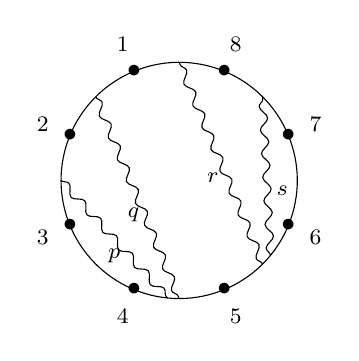
\begin{tikzpicture}[rotate=67.5,baseline=(current bounding box.east)]
	\begin{scope}
	\drawWLD{8}{1.5}
	\drawnumbers
	\drawlabeledprop{1}{0}{4}{0}{\footnotesize $q$ \quad}
	\drawlabeledprop{2}{0}{4}{-1}{\footnotesize  $p$}
    \drawlabeledprop{5}{0}{8}{0}{\footnotesize $r$ \ \ }
    \drawlabeledprop{5}{1}{7}{0}{\footnotesize \quad \ $s$}
		\end{scope}
	\end{tikzpicture}\]

To construct $I_1$ we start at vertex 1, so we set $i=1$, $j = 1$, and $I_1 = \emptyset$. 
\begin{itemize}
\item $j = 1$: Since $\Prop(1) = \{q,r\}$ and $r$ is the clockwise-most of these propagators, $r$ contributes at this step: $I_1(r)=1$. We let $I_1 = \{1\}$ and remove propagator $r$ from the diagram. 
\item $j = 2$: $\Prop(2) = \{p,q\}$, with $q$ being the clockwise-most of these propagators, $q$ contributes at this step: $I_1(q)=1$. So $I_1 = \{1,2\}$ and propagator $q$ is removed.
\item $j = 3$: $\Prop(3) = \{p\}$, so now $I_i(p) = 3$ and $I_1 = \{1,2,3\}$. The propagator $p$ is removed. The only remaining propagator in the diagram is $s$.
\item $j = 4$: Since $p$ and $q$ were removed in earlier steps, we now have $\Prop(4) = \emptyset$.
\item $j = 5$: $\Prop(5) = \{s\}$, and we have $I_1 = \{1,2,3,5\}$ with $I_1(s) = 5$.
\end{itemize}
There are no propagators left in the diagram, so the algorithm terminates and we have ${I_1 = \{1,2,3,5\}}$, or $1235$ for short. 
%So the propagators are ordered $r,q,p,s$ with respect to $I_1$, and 
$I_1$ viewed as a function is given by
\[I_1: \cP \longrightarrow [n] : \quad I_1(r) = 1,\quad I_1(q) = 2, \quad I_1(p) = 3, \quad I_1(s) = 5.\]
Applying the algorithm for all 8 starting vertices, we obtain the sets
\[1235, 2356, 3456, 4567, 5671, 6712, 7812, 8123.\]
The reader can easily verify that this sequence of $k$-sets satisfies the definition of a Grassmann necklace, and can (with significantly more work) also verify that this Grassmann necklace defines the positroid $M(W)$ associated to the Wilson loop diagram $W$ above. We will prove this in general shortly.
\end{eg}

%
%\begin{dfn} \label{prop order dfn}
%Given a set $\cP$ of $k$ propagators defining a Wilson loop diagram $(\cP, [n])$, the Grassmann necklace element $I_i$ imposes an ordering on it $\cP^i = \{p_1 \ldots p_k\}$ where $p_m$ is the $m^{th}$ propagator to contribute to $I_i$. We write $\cP_m^i = \{p_1 \ldots p_m\}$ to be the first $m$ propagators that contribute to $I_i$. We drop the superscript if the Grassman necklace element is clear.
%\end{dfn}

%In the sequel, when we refer to orderings on propagators, we refer to the ordering $\cP^i$. 

\begin{rmk} \label{clockwise ordering rem}
When $p$ contributes $I_i(p) = a$, it must be the clockwise-most propagator supported on $a$ that has not yet contributed to $I_i$. i.e. any propagator supported on $a$ that appears later in the ordering given by $I_i$ must be inside $(p, <_{a})$.
\end{rmk} 

\begin{rmk}\label{rmk algorithm locally same}
The following observation about the local behavior of the algorithm will be very useful in many of the arguments below.

Suppose we are going through the algorithm to construct $I_i^W$ for some $i$, and we are currently at step $j$ of the loop. Consider the diagram $W'$ formed by removing from $W$ all propagators that have already contributed to $I_i^W$. (This just replicates the behavior of the algorithm, which removes each propagator once it contibutes to $I_i^W$.)  Now suppose for some other diagram $V$ on the same vertex set we are constructing $I_m^V$ for some $m$, and we are at step $j$ of the loop, for the same $j$ as above.  Again obtain $V'$ from $V$ by removing all propagators assigned so far.

With this setup, if we can find a vertex $\ell$ occurring after both $i$ and $m$ such that the \emph{configuration} of propagators ending in the interval $[j-1, \ell+1]$ is identical in both $W'$ and $V'$, then the vertices contributed to $I_i^W$ and $I_m^V$ are the same from step $j$ to step $\ell$ (inclusive). See Figure~\ref{fig:locally identical} for an illustration of this.

Furthermore, if the propagators of $W'$ and $V'$ ending in the interval $[j-1, \ell+1]$ are also identically labelled, then $I_i^W$ and $I_m^V$ are the same as functions when restricted to those propagators.

\begin{figure}
\[
\begin{tikzpicture}[baseline=(current bounding box.east)]
  \begin{scope}
  W' = \drawWLDfragment[12]{3}{0.4} 
  %\drawnumberspartial % use this to debug
  \newnode[left]{1}{i}
  \newnode[below]{4}{j}
  \newnode{5}{}
  \newnode{6}{}
  \newnode{7}{}
  \newnode{8}{}
  \newnode{9}{}
  \newnode{11}{}
  \newnode[right]{12}{l+1}
  \begin{scope}
    \clipcenterarc(0,0)(\startpoint-10:\endpoint+10:\radius)
    \newpropbend{5.3}{7.6}{80}
    \node at (\zero + 6.5*\step:\radius*0.8) {\footnotesize $r$};
    \newprop[midway,left]{8.5}{-4}{}
    \node at (\zero + 8.15*\step:\radius*0.5) {\footnotesize $p$};
    \newprop[midway]{11.5}{-4}{}
    \node at (\zero + 12.2*\step:\radius*0.7) {\footnotesize $q$};
  \end{scope}
\end{scope}
\end{tikzpicture}
\qquad \qquad
\begin{tikzpicture}[baseline=(current bounding box.east)]
  V' = \begin{scope}
  \drawWLDfragment[12]{3}{0.4} 
  %\drawnumberspartial % use this to debug
  \newnode[left]{2}{m}
  \newnode[below]{4}{j}
  \newnode{5}{}
  \newnode{6}{}
  \newnode{7}{}
  \newnode{8}{}
  \newnode{9}{}
  \newnode{11}{}
  \newnode[right]{12}{l+1}
  \begin{scope}
    \clipcenterarc(0,0)(\startpoint-10:\endpoint+10:\radius)
    \newpropbend{5.3}{7.6}{80}
    \node at (\zero + 6.5*\step:\radius*0.8) {\footnotesize $r$};
    \newprop[midway,left]{8.5}{22}{}
    \node at (\zero + 8.5*\step:\radius*0.5) {\footnotesize $s$};
    \newprop[midway]{11.5}{21}{}
    \node at (\zero + 11.8*\step:\radius*0.8) {\footnotesize $t$};
  \end{scope}
\end{scope}
\end{tikzpicture}
\]
\caption{$W'$ and $V'$ are locally the same between $j$ and $l+1$, so we will have $I_i^W\cap [j,l] = I_m^V\cap[j,l]$ even though $p \neq s$ and $q \neq t$. Note that propagators such as $r$ which have {\em both} ends inside the region of interest must be identical in both diagrams.}\label{fig:locally identical}
\end{figure}

\end{rmk}

With that in mind, we are ready to begin proving properties of the algorithm. We first show that the algorithm for $I_i$ can never reach the final vertex (in the $<_i$ order) in a propagator's support without having already assigned that propagator; in particular, this guarantees that the construction of $I_i$ always terminates in fewer than $n$ steps.

\begin{lem}\label{lem no fourth vertex}
Let $W$ be an admissible Wilson loop diagram containing at least one propagator. For any $i \in [n]$ and for any $p \in \cP$, $I_i(p)$ is not maximal (with respect to $<_i$) amongst the vertices that support $p$.
\end{lem} 
\begin{proof}
Suppose for contradiction that we have $i \in [n]$ and $p \in \cP$ such that $I_i(p)$ is $<_i$-maximal in $V(p)$. There are two possibilities, which are illustrated in Figure~\ref{fig:no fourth vertex}: either $p = (i-1,b)$ for some $b$ (so $i$ and $I_i(p) = i-1$ are the two ends of a single edge), or $p = (a,b)$ with $i\leq_i a <_i b$ and $I_i(p) = b+1$. 

\begin{figure}

\[
\begin{tikzpicture}[baseline=(current bounding box.east),rotate = -18]
	\begin{scope}
	\drawWLDfragment[20]{2}{1}
	%\drawnumbers % use this to debug
	\newnode[left]{4}{I_i(p) = i-1}
	\newnode[left]{5}{i}
	\newnode[left]{7}{c}
	\newnode[left]{8}{}
	\newnode[right]{15}{b}
	\newnode[right]{16}{b+1}
	\newprop[midway,above]{4.7}{15.7}{\scriptsize $p$}
	\newprop[midway,below]{7.5}{15.3}{\scriptsize $q$}
      \draw[smallpropagator,light-gray] (\zero +\step *4.3:\radius*1) -- (90:\radius*0.5); 
	\node at (270+18:\radius*1.5) {\em Case 1};
	% \begin{scope}
	% \clip (\zero + 5*\step:\radius*1.1) rectangle (90:\radius*0.8);
	% \draw[smallpropagator,color=gray] (\zero+4.5*\step:\radius) -- (\zero + 19*\step:\radius);
	% \end{scope}
		\end{scope}
	\end{tikzpicture}
\qquad \qquad 
	\begin{tikzpicture}[baseline=(current bounding box.east),rotate = 36]
	\begin{scope}
	\drawWLDfragment[20]{2}{1}
	%\drawnumbers % use this to debug
	\newnode[left]{4}{a}
	\newnode[left]{5}{}
	\newnode[left]{7}{}
	\newnode[left]{8}{}
	\newnode[right]{15}{b}
	\newnode[right]{16}{b+1 = I_i(p)}
	\newnode[right]{11}{d}
	\newnode[below]{12}{}
	\newnode[left]{2}{i}
	\newprop[midway,above]{4.5}{15.7}{\scriptsize $p$}
		\node at (270-36:\radius*1.5) {\em Case 2};
	\begin{scope}
	\clip (0,0) circle (\radius);
	%q
	\draw[smallpropagator] (\zero+11.5*\step:\radius*1.2) to [bend left = 45] (\zero + 15.5*\step:\radius*1.2); 
	\node at (\zero + 13.5*\step:\radius*0.55) {\scriptsize $q$};
	%r
	\draw[smallpropagator] (\zero+7.5*\step:\radius*1.2) to [bend left = 45] (\zero + 11.4*\step:\radius*1.2);
	\node at (\zero + 9.5*\step:\radius*0.55) {\scriptsize $r$};

	\end{scope}
		\end{scope}
	\end{tikzpicture}
\] 
\caption{The two types of configuration that would (in theory) allow the propagator $p$ to contribute its $<_i$-maximal support vertex to $I_i$.}
\label{fig:no fourth vertex}
\end{figure}
In Case 1, observe that we must have another propagator $q = (c,b)$ with $c<_i b$ and $I_i(q) = b+1$, because otherwise $I_i$ would assign $p$ to $b+1$. Now $q$ also contributes the $<_i$-maximal vertex in its support to $I_i$ and is an instance of Case 2. Therefore it suffices to show that no admissible Wilson loop diagram admits the configuration illustrated in Case 2 of Figure~\ref{fig:no fourth vertex}. 

So let $p = (a,b)$ with $a<_ib$ and $I_i(p) = b+1$, and choose $p$ such that $\big|[a+1,b]\big|$ is minimal amongst propagators of $W$ which contribute their last vertex and are in Case 2.

Since $I_i(p) \neq b$, there must exist a propagator $q$ inside of $(p,<_i)$ with $I_i(q) = b$. The propagator $q$ cannot end on the edge $b-1$, as this would contradict the minimality of $p$, so we have $q = (d,b)$ with $a <_i d <_i b$, and $I_i(q) = b$. 

In order for $q$ to remain unassigned until vertex $b$, there must be another propagator $r$ with an end on edge $d$ and $I_i(r) = d+1$; the only way this can occur is if $r$ is outside of $(q,<_i)$ but inside $(p,<_i)$. But now $r$ contributes its fourth vertex to $I_i$, again contradicting the minimality of $p$.
\end{proof}

\begin{cor}\label{GN alg well defined}
If $W$ is an admissible Wilson loop diagram with $k$ propagators and $n$ vertices, then Algorithm~\ref{alg:put GN on WLD} assigns exactly $k$ distinct vertices to each $I_i$ in $n$ steps.
\end{cor} 
\begin{proof}
Fix $i \in [n]$. It follows from the proof of Lemma~\ref{lem no fourth vertex} that in applying Algorithm~\ref{alg:put GN on WLD} to construct the set $I_i$, the algorithm can never reach the fourth vertex of a propagator's support (ordered with respect to $<_i$) without having already assigned that propagator. Therefore if the algorithm starts at vertex $i$, all propagators must have been eliminated by the time it gets to vertex $i-1$, ensuring that the algorithm is completed in less than one full circumnavigation of the diagram and that $I_i$ contains exactly $k$ distinct elements.
\end{proof}

We now reverse our perspective and ask: given a propagator $p$ and a vertex $i$ in the support of $p$, for which set of starting vertices does the algorithm assign $p$ to $i$? 






Specifically, for each $i$ in the support of $p$ we define the set
\[J_p^{W}(i) = \{m \in [n] \ | \ I^{W}_m(p) = i \},\]
i.e. the set of starting vertices $m$ such that $I_m^{W}$ assigns $p$ to $i$. 

The following lemma establishes that these sets behave in a simple and predictable manner, a fact which we will repeatedly use in subsequent proofs.




\begin{lem} \label{vertex cyclic int lem}
  
Let $W = (\cP,[n])$ be an admissible Wilson loop diagram.  For every $p = (i,j) \in \cP$, the sets $J_p^{W}(i)$, $J_p^{W}(i+1)$, $J_p^{W}(j)$, and $J_p^{W}(j+1)$ are each non-empty cyclic intervals which partition $[n]$ and occur in the given cyclic order.
\end{lem}

\begin{rmk}\label{rmk cyclic}
  Before the proof, let us observe that one of the main ways that the above lemma will be used is in observations like the following.  Suppose $p=(i,j)$ is a propagator and $I_{j+1}(p) = j+1$.  Consider $I_{j+2}(p)$.  Since $j+1$ is the last vertex in the $j+2$ order, $p$ can not contribute $j+1$ to $I_{j+2}$, so the fact that the invervals in the statement of the lemma are non-empty and occur in their cyclic order implies that $I_{j+2}(p)=i$.  More generally, whenever we know that a propagator stops contributing a particular vertex, then we know that it must contribute its cyclically next vertex.  This little observation is surprisingly useful, to the point that the details which appear in the proof of Lemma~\ref{vertex cyclic int lem} are never needed again: the mere fact of non-empty intervals in the correct order suffices.
\end{rmk}
  
Now we proceed to the proof of Lemma~\ref{vertex cyclic int lem}.

\begin{proof}
We will prove the result by induction on the number of propagators.  If $W$ has one propagator then the result is immediate.  Now suppose $W$ has more than one propagator.  Since non-supporting vertices have no effect on Algorithm~\ref{alg:put GN on WLD}, it suffices to prove the result for $W$  (possibly weakly admissible) with no non-supporting vertices.  Then by Lemma~\ref{lem sian}, $W$ has at least one of the four situations illustrated in Figure~\ref{fig 3 cases}.

\begin{figure}
\begin{tabular}{lll}
% case 1
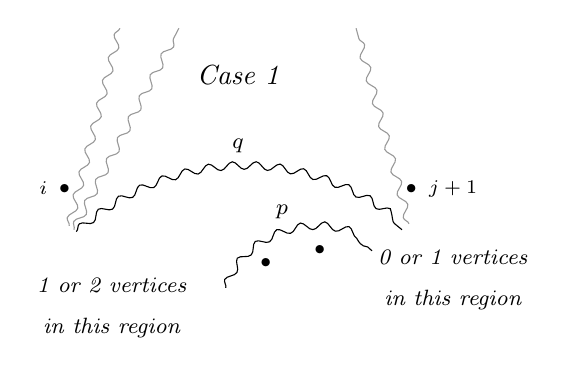
\begin{tikzpicture}[baseline=(current bounding box.east)]
	\begin{scope}
	\drawWLDfragment[8]{3}{0.3} % draws the arc and sets up the parameters
	%\drawnumbers % use this to debug
	% next two lines draw the highlighted regions
	\centerarc[linehighlight](0,0)(\zero + 1.85*\step:\zero + 4.4*\step:\radius)
	\centerarc[linehighlight](0,0)(\zero + 6.75*\step:\zero + 7.4*\step:\radius)
	% labels explaining the highlighted regions
	\node[align = center] at (\zero + 2.7*\step:\radius*1.3) {\em \footnotesize 1 or 2 vertices \\[3pt] \em \footnotesize in this region};
	\node[align = center] at (\zero + 7.5*\step:\radius*1.4) {\em \footnotesize 0 or 1 vertices \\[3pt]\em \footnotesize in this region};
	\begin{scope} % this scope draws the propagators and their labels
		\clipcenterarc(0,0)(\startpoint-20:\endpoint+20:\radius)
		%q
		\draw[smallpropagator] (\zero+1.65*\step:\radius*1.1) to [bend left = 40] (\zero + 7.4*\step:\radius*1.1); 
		%p
		\draw[smallpropagator] (\zero+4.3*\step:\radius*1.1) to [bend left = 55] (\zero + 6.8*\step:\radius*1.1); 
		\draw[smallpropagator,light-gray] (\zero+1.5*\step:\radius*1.1) -- (180:\radius*0.5); 
		\draw[smallpropagator,light-gray] (\zero+1.6*\step:\radius*1.1) -- (180:\radius*0.25);
		\draw[smallpropagator,light-gray] (\zero+7.55*\step:\radius*1.1) -- (0:\radius*0.5); 
		%\draw[smallpropagator,light-gray] (\zero+7.5*\step:\radius*1.1) -- (0:\radius*0.25);  
		\node at (\zero + 4.5*\step:\radius*0.5){\footnotesize $q$};
		\node at (\zero + 5.5*\step:\radius*0.8){\footnotesize $p$};
	\end{scope}
	% draw the nodes
	\newnode[left]{1}{i}
	\newnode[right]{8}{j+1}
	\newnode[below]{5}{}
	\newnode[below]{6}{}
% case label
\node at (270:\radius*0.2) {\em Case 1};
\end{scope}
\end{tikzpicture}
%
%
%
& \qquad \qquad &
%
%
%
% case 2
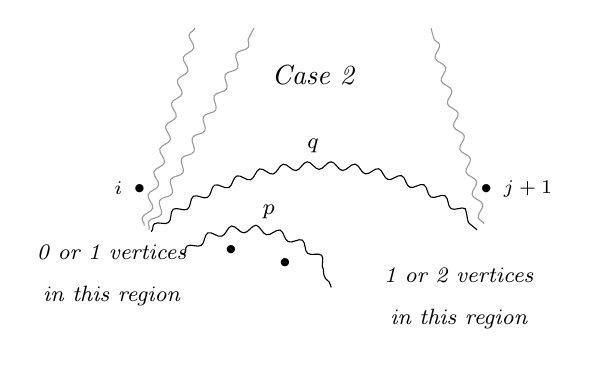
\begin{tikzpicture}[baseline=(current bounding box.east)]
\begin{scope}
	\drawWLDfragment[8]{3}{0.3} % draw arc
	%\drawnumbers % use this to debug
	% highlighted regions
	\centerarc[linehighlight](0,0)(\zero + 1.85*\step:\zero + 2.4*\step:\radius)
	\centerarc[linehighlight](0,0)(\zero + 4.75*\step:\zero + 7.4*\step:\radius)
	%labels for highlighted regions
	\node[align = center] at (\zero + 6.6*\step:\radius*1.3) {\em \footnotesize 1 or 2 vertices \\[3pt]\em \footnotesize in this region};
	\node[align = center] at (\zero + 1.6*\step:\radius*1.35) {\em \footnotesize 0 or 1 vertices \\[3pt]\em \footnotesize in this region};
	% draw props and their labels
	\begin{scope}
		\clipcenterarc(0,0)(\startpoint-20:\endpoint+20:\radius)
		%q
		\draw[smallpropagator] (\zero+1.65*\step:\radius*1.1) to [bend left = 40] (\zero + 7.4*\step:\radius*1.1); 
		%p
		\draw[smallpropagator] (\zero+2.3*\step:\radius*1.1) to [bend left = 55] (\zero + 4.8*\step:\radius*1.1); 
		\draw[smallpropagator,light-gray] (\zero+1.5*\step:\radius*1.1) -- (180:\radius*0.5); 
		\draw[smallpropagator,light-gray] (\zero+1.6*\step:\radius*1.1) -- (180:\radius*0.25);
		\draw[smallpropagator,light-gray] (\zero+7.55*\step:\radius*1.1) -- (0:\radius*0.5); 
		%\draw[smallpropagator,light-gray] (\zero+7.5*\step:\radius*1.1) -- (0:\radius*0.25);  
		\node at (\zero + 4.5*\step:\radius*0.5){\footnotesize $q$};
		\node at (\zero + 3.5*\step:\radius*0.8){\footnotesize $p$};
	\end{scope}
	% nodes
	\newnode[left]{1}{i}
	\newnode[right]{8}{j+1}
	\newnode[below]{3}{}
	\newnode[below]{4}{}
	% case label
	\node at (270:\radius*0.2) {\em Case 2};
\end{scope}
\end{tikzpicture}
%
%
%
\\
\ & \ & \ \\
%
%
%
% case 3
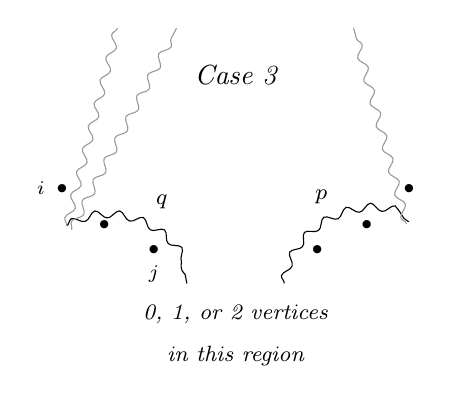
\begin{tikzpicture}[baseline=(current bounding box.east)]
\begin{scope}
	\drawWLDfragment[8]{3}{0.3} % draw arc
	%\drawnumbers % use this to debug
	% highlight region
	\centerarc[linehighlight](0,0)(\zero + 3.6*\step:\zero + 5.4*\step:\radius)
	% region label
	\node[align = center] at (\zero + 4.5*\step:\radius*1.3) {\em \footnotesize 0, 1, or 2 vertices \\[3pt]\em \footnotesize in this region};
	% scope to draw props and their labels
	\begin{scope}
		\clipcenterarc(0,0)(\startpoint-20:\endpoint+20:\radius)
		%q
		\draw[smallpropagator] (\zero+1.5*\step:\radius*1.1) to [bend left = 55] (\zero + 3.7*\step:\radius*1.1); 
		%p
		\draw[smallpropagator] (\zero+5.3*\step:\radius*1.1) to [bend left = 55] (\zero + 7.6*\step:\radius*1.1); 
		\draw[smallpropagator,light-gray] (\zero+1.5*\step:\radius*1.1) -- (180:\radius*0.5); 
		\draw[smallpropagator,light-gray] (\zero+1.6*\step:\radius*1.1) -- (180:\radius*0.25);
		\draw[smallpropagator,light-gray] (\zero+7.55*\step:\radius*1.1) -- (0:\radius*0.5); 
		%\draw[smallpropagator,light-gray] (\zero+7.5*\step:\radius*1.1) -- (0:\radius*0.25);  
		\node at (\zero + 2.8*\step:\radius*0.8){\footnotesize $q$};
		\node at (\zero + 6.5*\step:\radius*0.8){\footnotesize $p$};
	\end{scope}
	% draw nodes
	\newnode[left]{1}{i}
	\newnode[below]{2}{}
	\newnode[below]{3}{j}
	\newnode[below]{6}{}
	\newnode[below]{7}{}
	\newnode[right]{8}{}
	% case label
	\node at (270:\radius*0.2) {\em Case 3};
\end{scope}
\end{tikzpicture}
%
%
%
& \qquad \qquad & \qquad
%
%
%
% case 4
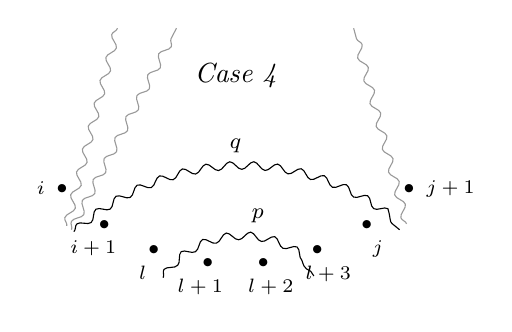
\begin{tikzpicture}[baseline=(current bounding box.east)]
	\begin{scope}
	\drawWLDfragment[8]{3}{0.3} % draw arc
	%\drawnumbers % use this to debug
	%scope to draw props and their labels
	\begin{scope}
		\clipcenterarc(0,0)(\startpoint-20:\endpoint+20:\radius)
		%q
		\draw[smallpropagator] (\zero+1.65*\step:\radius*1.1) to [bend left = 40] (\zero + 7.4*\step:\radius*1.1); 
		%p
		\draw[smallpropagator] (\zero+3.3*\step:\radius*1.1) to [bend left = 55] (\zero + 5.8*\step:\radius*1.1); 
		\draw[smallpropagator,light-gray] (\zero+1.5*\step:\radius*1.1) -- (180:\radius*0.5); 
		\draw[smallpropagator,light-gray] (\zero+1.6*\step:\radius*1.1) -- (180:\radius*0.25);
		\draw[smallpropagator,light-gray] (\zero+7.55*\step:\radius*1.1) -- (0:\radius*0.5); 
		%\draw[smallpropagator,light-gray] (\zero+7.5*\step:\radius*1.1) -- (0:\radius*0.25);  
		\node at (\zero + 4.5*\step:\radius*0.5){\footnotesize $q$};
		\node at (\zero + 5*\step:\radius*0.8){\footnotesize $p$};
	\end{scope}
	% draw nodes
	\newnode[left]{1}{i}
	\newnode[below]{2}{i+1\quad }
	\newnode[below]{3}{l\quad}
	\newnode[below]{4}{l+1\ \ }
	\newnode[below]{5}{\ \ l+2}
	\newnode[below]{6}{\quad l+3}
	\newnode[below]{7}{\quad j}
	\newnode[right]{8}{j+1}
	% case label
	\node at (270:\radius*0.2) {\em Case 4};
\end{scope}
\end{tikzpicture}
\end{tabular}
    \caption{Four cases for admissible WLDs with no non-supporting vertices. The gray half-propagators illustrate where propagators may occur, but are not required to exist.}\label{fig 3 cases}
  \end{figure}


In each of the four cases, when we remove the propagator labelled $p$ we obtain a diagram which satisfies the statement of the theorem by the induction hypothesis, and contains a propagator ${q = (i,j)}$ with no other propagators inside it (with respect to the $<_i$ orientation). Note that this region may or may not contain non-supporting vertices, which we will call $l, l+1, \ldots$ as necessary. Let $V$ be the diagram obtained by removing the propagator $p$ from $W$ (Figure \ref{fig V diagram}). $V$ is guaranteed to be an admissible diagram, since it was formed by removing a propagator from a diagram that was at least weakly admissible.

Consider Case 4 of Figure~\ref{fig 3 cases} first, as it is the easiest.  In this case, the vertices ${\{l,l+1,l+2,l+3\}}$ which support $p$ in $W$ are non-supporting in $V$, so for every propagator $r$ in $V$ (including $q$) we have $J_r^{V} = J_r^{W}$; these are non-empty cyclic intervals in the correct order by the induction hypothesis.  Additionally, it is clear from Figure~\ref{fig 3 cases} that $J_p^{W}(l+a) = \{l+a\}$ for $a\in\{1,2,3\}$ and $J_p^{W}(l) = [n] \backslash \{l+1, l+2, l+3\}$. The result therefore holds in this case.


Now we proceed to consider the first three cases of Figure~\ref{fig 3 cases}.
We first describe $J_q^{V}(*)$, which can be handled identically for all three cases.

In $V$ there are no propagators inside $q$ by construction, so we see from Figure \ref{fig V diagram} that
\[l, l+1, \ldots ,j \in J^{V}_q(j) \text{ (if $l$ exists) and }  j+1 \in J^{V}_q(j+1).\]
Note that $j+2 \not\in J^{V}_q(j+1)$ by Lemma~\ref{lem no fourth vertex}, so  $J^{V}_q(j+1) = \{j+1\}$ and by the induction hypothesis we must have $j+2 \in J^{V}_q(i)$. Thus there exist vertices $d,e \in [j+2,i+1]$ with $d <e$, such that
\ba J^{V}_q(i) = [j+2,d-1], \quad J^{V}_q(i+1) = [d,e-1], \quad J^{V}_q(j) = [e,j], \quad J^{V}_q(j+1) = \{j+1\}, \label{deeqs}\ea
and all intervals are non-empty.

We now consider what happens as we move from $V$ to each of the three remaining cases for $W$. We need to consider both $J^{W}_p$ and $J^{W}_r$ for $r \neq p$, since the addition of $p$ can have a knock-on effect on later steps in the algorithm.


\begin{figure}[h]
\[
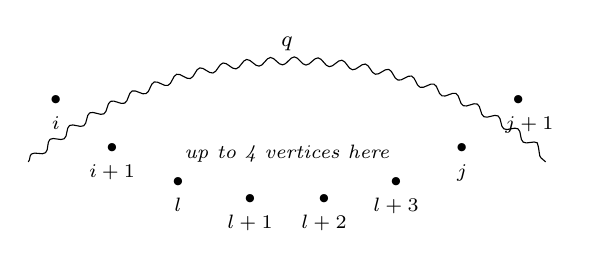
\begin{tikzpicture}[baseline=(current bounding box.east)]
	\begin{scope}
	\drawWLDfragment[8]{4}{0.3}
	%\drawnumbers % use this to debug
	%\clip (\zero + 1.5*\step:1.5*\radius) rectangle (345:{\radius});
	\centerarc[linehighlight](0,0)(\zero + 2.8*\step:\zero + 6.2*\step:\radius)
	\newnode[below]{1}{i}
	\newnode[below]{2}{i+1}
	\newnode[below]{3}{l}
	\newnode[below]{4}{l+1}
	\newnode[below]{5}{l+2}
	\newnode[below]{6}{l+3}
	\newnode[below]{7}{j}
	\newnode[below]{8}{\quad j+1}
	%\node[rotate=-15] at (\zero + 2.7*\step:\radius) {\Large $($};
	%\node[rotate=15] at (\zero + 6.3*\step:\radius) {\Large $)$};
	\node at (\zero + 4.5*\step:\radius*0.85) {\em \scriptsize up to 4 vertices here};
	\begin{scope}
	\clipcenterarc(0,0)(\startpoint-10:\endpoint+10:\radius)
		\draw[smallpropagator] (\zero+1.3*\step:\radius*1.2) to [bend left = 40] (\zero + 7.7*\step:\radius*1.2); 
	\node at (\zero + 4.5*\step:\radius*0.5){\footnotesize $q$};
\end{scope}
\end{scope}
\end{tikzpicture}
\]
\caption{Diagram $V$ is $W$ with $p$ removed; there are no propagators inside $q = (i,j)$, though there may be up to 4 non-supporting vertices labelled $l, l+1, \ldots$.}
\label{fig V diagram}
\end{figure}

%%%%%%%%%

\textbf{Cases 1 and 2}: These cases behave essentially identically (except when $j$ or $j+1$ are not in the support of $p$, which can occur in Case 2 only; see below) so we handle the majority of the proof for these two cases simultaneously. Write $p=(m,m+2)$ where $m\in \{i, i+1, l\}$. Let $1\leq a\leq 3$ be the number of non-supporting vertices inside $q$ in $V$ (note that there is at least 1); so these vertices are $l, \ldots, l+a-1$.  Note that these vertices are non-supporting in $V$ but are all in the support of $p$ in $W$. 

We first calculate $I^{W}_w$ for a starting vertex ${w \in [n]\backslash \{l, l+1, \ldots,j,j+1\}}$. Note that $p$ has no effect on other propagators for starting vertices in this range (since $p$ will be the final propagator encountered by the algorithm) so if $r \neq p$, then $I_w^W(r) = I_w^V(r)$. Meanwhile, the value of $I^{W}_w(p)$ depends on which step in the algorithm the propagator $q$ contributes a vertex in the diagram $V$, i.e. on the value of $I^{V}_w(q)$. Thus, if $w\in J_q^{V}(i)$ then 
    \[
    I_w^{W}(r) =  \begin{cases}
        \max\{i+1, m\} & \text{if } r=p \\
        I_{w}^{V}(r) & \text{if } r\neq p
      \end{cases} 
    \]
    while if $w\in J_q^{V}(i+1)$ or $w\in J_q^{V}(j)$ then
    \[
    I_w^{W}(r) =  \begin{cases}
        l & \text{if } r=p \\
        I_{w}^{V}(r) & \text{if } r\neq p
      \end{cases} 
      \]
We also need to understand $I^{W}_w$ for $w \in \{l,l+1,\ldots,j,j+1\}$. For the majority 
%$w \in [l, l+a-1]$} 
%I left this as a comment so we can add it in if necessary, but I don't think we need this level of precision in this sentence: we're just signposting what we're going to do in detail shortly.
of these vertices, we use the following observation: if $p$ is the first propagator to be assigned a value by $I_w^{W}$, then the remainder of $I_w^{W}$ proceeds identically to the assignments of $I^{V}_{w+1}$ (recall Remark~\ref{rmk algorithm locally same}).  Thus we have for any $0\leq b <a$
    \[
    I_{l+b}^{W}(r) = \begin{cases}
      l+b & \text{if } r=p\\
      I_{l+b+1}^{V}(r) & \text{if } r\neq p
    \end{cases}
    \]
Similarly, if $j$ is in the support of $p$, then we have
     \[
       I_j^{W}(r) = \begin{cases}
         j & \text{if $r=p$ and $j$ is in the support of $p$}\\
         I_{j+1}^{V}(r) & \text{if $r\neq p$ and $j$ is in the support of $p$}\\
       \end{cases}
       \]
If $j$ is not in the support of $p$, then we must be in Case 2 of Figure~\ref{fig 3 cases} with two vertices in the right hand region.  In this case, if we start the algorithm at $j$ we need to know whether there will be any unassigned propagators other than $p$ when we reach vertex $i$, so as to know what $p$ contributes.

Consider the Wilson loop diagram $X$ formed from $V$ by replacing the propagator $q = (i,j)$ with $q = (i, j-1)$;  $X$ is still admissible since we have not decreased the support of any set of propagators. 
% From the diagram we can see that $J_{j}^{V}(r) = J_{j}^{X}(r)$ for all $r\neq p$ (and in particular for $r=q$) and $J_{j}^{X}(r) = J_{j+1}^{X}(r)$ for $r\neq q,p$.  
It follows from the position of $q$ in $X$ that $I_j^X(q) = j$, and from Lemma~\ref{lem no fourth vertex} that $I_{j+1}^X(q) \neq j$. By the induction hypothesis, we must therefore have $I_{j+1}^X(q) = i$; in particular, this means that if we start at $j+1$ and assign propagators to vertices according to the algorithm, when we reach vertex $i$ in $X$ all propagators other than $q$ must have been assigned.

Therefore if we start at $j$ in $W$, we first assign $q$ to $j$ then proceed to assign as in $X$ starting at $j+1$, and hence when we get to $i$ the only remaining unassigned propagator is $p$. We obtain
       \[
       I_j^{W}(r) = \begin{cases}

       m & \text{if $r =p$ and $j$ is not in the support of $p$} \\
       I_{j}^{V}(r) & \text{if $r\neq p$ and $j$ is not in the support of $p$}\end{cases}
       \] 
This completes the analysis of $I_j^W$. Finally, we consider what happens when we start the algorithm at vertex $j+1$. If $j+1$ is in the support of $p$ then we can argue as above to get
\[
       I_{j+1}^{W}(r)  = \begin{cases}
         j+1 & \text{if $r=p$ and $j+1$ is in the support of $p$}\\
         I_{j+2}^{V}(r) & \text{if $r\neq p$ and $j+1$ is in the support of $p$}.
       \end{cases}
       \]
Now suppose $j+1$ is not in the support of $p$. If we start at $j+1$ we need to know whether there are any unassigned propagators supported on edge $i$ when we reach vertex $i$. We already know that $J_q^{V}(j+1) = \{j+1\}$; in particular this means that $q$ contributes $i$ in $I_{j+2}^{V}$, by the induction hypothesis applied to $V$. However the construction of $I^{V}_{j+1}$ first assigns $q$ to $j+1$ and then proceeds identically to $I^{V}_{j+2}$.  In particular if $i$ was assigned in $I^{V}_{j+1}$, then it would not be available to assign to $q$ in $I^{V}_{j+2}$ as all other propagators supported at $i$ in $V$ come before $q$. 

Therefore $p$ is the only potentially unassigned propagator on edge $i$ when we reach vertex $i$ in the algorithm for $I_{j+1}^W$, and
    \[
    I_{j+1}^{W}(r)  = \begin{cases}
      m & \text{if  $r=p$ and $j+1$ is not in the support of $p$}\\
      I_{j+1}^{V}(r) & \text{if  $r\neq p$ and $j+1$ is not in the support of $p$}
    \end{cases}
    \]
We can now describe the intervals $J^{W}_r(*)$ for Cases 1 and 2 of Figure~\ref{fig 3 cases}. For $r \neq p$ the intervals are clearly still cyclic and appear in the correct order, and we can assemble the intervals for the $J_p^{W}(*)$ as follows. Recall that $p = (m,m+2)$, $1 \leq a \leq 3$ is the number of non-supporting vertices inside $q$ in $V$, and these non-supporting vertices are denoted $\{l,l+1, \dots\}$. 
    \begin{itemize}
      \item 
    If $m=l$ then either $a=2$ (so $l+1=m+1$, $j=m+2$, and $j+1=m+3$) or $a=3$ (so $l+1=m+1$, $l+2=m+2$, $j=m+3$, and $j+1$ is not in the support of $p$), and in both cases
    \begin{gather*}
    J^{W}_p(m) = [m+4, m], \qquad  J^{W}_p(m+1) = \{m+1\}, \\ J^{W}_p(m+2) = \{m+2\}, \qquad  J^{W}_p(m+3) = \{m+3\},
    \end{gather*}
    which are nonempty and otherwise as required.
  \item
        If $m=i+1$ then checking each of the three different possibilities for $a$ we likewise get
    \begin{gather*}
    J^{W}_p(m) = [m+4, d-1], \qquad  J^{W}_p(m+1) = [d, m+1], \\  J^{W}_p(m+2) = \{m+2\}, \qquad  J^{W}_p(m+3) = \{m+3\},
    \end{gather*}
    which are nonempty and otherwise as required. Recall that $d$ was defined in equation \eqref{deeqs}.
  \item If $m=i$ then $a=1$ or $a=2$, in the former case $l=m+2$, $j=m+3$ and $j+1$ is not in the support of $p$ so
    \begin{gather*}
    J^{W}_p(m) = \{m+4\}, \qquad  J^{W}_p(m+1) = [m+5, d-1], \\  J^{W}_p(m+2) = [d, m+2], \qquad  J^{W}_p(m+3) = \{m+3\},
    \end{gather*}
    while in the latter $l=m+2$, $l+1=m+3$, and $j$ and $j+1$ are not in the support of $p$ so
    \begin{gather*}
    J^{W}_p(m) = [m+4, j+1], \qquad  J^{W}_p(m+1) = [j+2, d-1], \\  J^{W}_p(m+2) = [d, m+2], \qquad  J^{W}_p(m+3) = \{m+3\},
    \end{gather*}
    which are again as required.
    \end{itemize}

\textbf{Case 3}: In this case there are no non-supporting vertices $l, l+1, \ldots$ inside $q$.  Again write $p=(m, m+2)$ where $m\in \{j, j+1, j+2\}$. We proceed as in the previous cases, by computing $I^{W}_w$ for vertices $w$ in roughly increasing order of difficulty.

For $w \in [n]\backslash\{j+1,m,m+1,m+2,m+3\}$: if $w\in J_q^{V}(i)$ or $w\in J_q^{V}(i+1)$ then
    \[
    I_w^{W}(r) =  \begin{cases}
        m & \text{if } r=p \\
        I_{w}^{V}(r) & \text{if } r\neq p
      \end{cases} 
    \]
    while if $w\in J_q^{V}(j)$ then
    \[
    I_w^{W}(r) =  \begin{cases}
        \max\{m, j+1\} & \text{if } r=p \\
        I_{w}^{V}(r) & \text{if } r\neq p
      \end{cases} 
    \]

Finally, for $j+1$ and the vertices in the support of $p$, we have

\begin{align*}
  I_{j+1}^{W}(r) &= \begin{cases}
    j+1 & \text{if } r=q\\
    j+2 & \text{if } r=p\\
    I_{j+3}^{V}(r) & \text{if } r\neq p,q
  \end{cases}\\
  I_m^{W}(r) &= \begin{cases}
    m & \text{if $r=p$ and $q$ not supported on $m$}\\
    m+1 & \text{if $r=p$ and $q$ supported on $m$}\\
    I_{m}^{V}(r) & \text{if } r\neq p
  \end{cases}\\
  I_{m+1}^{W}(r) & = \begin{cases}
    m+1 & \text{if $r=p$ and $q$ not supported on $m+1$} \\
    m+2 & \text{if $r=p$ and $q$ supported on $m+1$} \\
    I_{m+1}^{V}(r) & \text{if } r\neq p,q
  \end{cases}\\
  I_{m+2}^{W}(r) & = \begin{cases}
    m+2 & \text{if } r=p \\
    I_{m+3}^{V}(r) & \text{if } r\neq p
  \end{cases}\\
  I_{m+3}^{W}(r) & = \begin{cases}
    m+3 & \text{if } r=p \\
    I_{m+4}^{V}(r) & \text{if } r\neq p
  \end{cases}
\end{align*}
Note that $I_{m+2}^{V}(r) = I_{m+3}^{V}(r)$ for all propagators $r$ in $V$, and that if $j+1\not\in\{m, m+1, m+2, m+3\}$ then $j+2$ and $j+3$ are non-supporting vertices in $V$, so in that case $I_{j+2}^{V}(r) = I_{j+3}^{V}(r) = I_{j+4}^{V}(r)$ for $r$ in $V$. 

Therefore, once again we can see that the $J_r^{W}(*)$ are cyclic for all $r\neq p$ in $W$.  Assembling the intervals for $p$ we have:
\begin{itemize}
\item If $m=j$ then
\begin{gather*}J_p^{W}(m) = [m+4,e-1], \qquad  J_p^{W}(m+1) = [e,m], \\  J_p^{W}(m+2) = [m+1,m+2], \qquad  J_p^{W}(m+3) = \{m+3\},\end{gather*}
Recall that $e$ was defined in equation \eqref{deeqs}.
\item If $m=j+1$ then
\begin{gather*}J_p^{W}(m) = [m+4,m-1], \qquad J_p^{W}(m+1) = [m,m+1], \\  J_p^{W}(m+2) = \{m+2\}, \qquad  J_p^{W}(m+3) = \{m+3\},\end{gather*}
\item If $m=j+2$ then
\begin{gather*}J_p^{W}(m) = [m+4,m], \qquad  J_p^{W}(m+1) = \{m+1\}, \\  J_p^{W}(m+2) = \{m+2\}, \qquad  J_p^{W}(m+3) = \{m+3\}.\end{gather*}
\end{itemize}
The result now follows by induction.
\end{proof}



We are now ready to prove that Algorithm~\ref{alg:put GN on WLD} does in fact give the Grassmann necklace of the positroid associated to $W$. We do this in two parts: Theorem~\ref{res:alg gives GN} verifies that the sets $(I_1,\dots,I_n)$ obtained from the algorithm do form a Grassmann necklace, and Theorem~\ref{res alg gives correct GN} proves that this Grassmann necklace defines the positroid $M(W)$.

\begin{thm}\label{res:alg gives GN}
The sequence of $k$-subsets $(I_1,\dots,I_n)$ obtained by applying Algorithm~\ref{alg:put GN on WLD} to all vertices of an admissible diagram $W$ is a Grassmann necklace.
\end{thm}
\begin{proof}
%\note{Sian replaced ``counterclockwise'' with ``clockwise'' in a couple of places in this proof: someone please doublecheck?  Karen checked and it seems correct with Sian's changes.}
% Thank you! Clocks are difficult.
For each $i \in [n]$, let $I_i$ be the set of vertices assigned to the propagators of $W$ by Algorithm~\ref{alg:put GN on WLD} with starting vertex $i$. By Lemma~\ref{GN alg well defined}, we know that $|I_i| = k$ for each $i \in [n]$. We prove that $I_{i+1} \supseteq I_i \backslash \{i\}$ for all $i \in [n]$; this is equivalent to the definition of Grassmann necklace given in Definition~\ref{def:grassmann necklace}.

Fix $n$, and suppose for a contradiction that there exists an admissible diagram for which there exists an $i$ with $m\in I_i\setminus \{i\}$ and $m \not\in I_{i+1}$.  Let $W$ be such a counterexample with the minimal number of propagators.

If $i \not\in I_i$, then there are no propagators supported on $i$ at all.  In this case it is clear that applying Algorithm~\ref{alg:put GN on WLD} at vertex $i$ and vertex $i+1$ produces exactly the same result, i.e. $I_{i+1} = I_i$, and so $W$ is not a counterexample at all.

Now suppose that $i \in I_i$.  Let $p$ be the propagator which contributes $i$ to $I_i$, that is $I^W_i(p) = i$; thus one end of $p$ must lie on either edge $i-1$ or edge $i$.  In both cases let $b$ denote the edge supporting the other end of $p$, i.e. $p = (i, b)$ or $p = (i-1, b)$.


\textbf{Case I}:  Suppose $p$ has one end on edge $i-1$. By Remark~\ref{rmk algorithm locally same} the construction of $I_i^W$ and $I_{i+1}^W$ is locally the same (indeed, locally {\em identical} in this case) from vertex $i+1$ to $b-1$, so we have $I_{i+1}^W \cap [i+1,b-1] = I_{i}^W \cap [i+1,b-1]$. Note that if $b = i+1$ then this interval is empty and the equality remains true.

%If $p$ is not supported on $i+1$, then in building $I_{i+1}$ we will assign the same propagators as in the construction of $I_i$ from vertices $i+1$ up to $b-1$, and in particular we have \bas I_{i+1} \cap [i+1,b-1] = I_{i} \cap [i+1,b-1]\eas by Remark \ref{rmk algorithm locally same}.  If $p$ is supported on $i+1$, then $b= i+1$ and the interval $[i+1,b-1]$ is empty, so the above equality remains true, albeit vacuously.  

By Lemma~\ref{vertex cyclic int lem} it must happen that we have $I_{i+1}^W(p) = b$, as otherwise $b$ would never be contributed by $p$.  Consequently, when the construction of $I_{i+1}^W$ reaches vertex $b$ there cannot be any remaining unassigned propagators that are supported on $b$ and clockwise of $p$ (Remark~\ref{clockwise ordering rem}). It follows that the same must be true when $I_i^W$ reaches vertex $b$, since $I_i^W$ and $I_{i+1}^W$ behave identically on the interval $[i+1,b-1]$ as noted in the previous paragraph. 

The previous two paragraphs also imply that $m \geq_i b+1$, since $I_{i+1}^W \cap [i+1,b-1] = I_{i}^W \cap [i+1,b-1]$ and $b \in I_{i+1}^W$.

%This is also true in when the algorithm constructing $I_i$ reaches $b$, \st{since the same propagators have been assigned beforehand.}\sanote{don't like same here}{\color{violet}since any propagators lying counterclockwise of $p$ on the edge $i-1$ must have their support in $[i-1, b]$. By Lemma \ref{lem no fourth vertex}, these propagators contribute before the algorithm reaches $b$. Furthermore, Remark  \ref{rmk algorithm locally same} implies that these propagators contribute the same vertices to both $I_i$ and $I_{i+1}$.} This also implies that $m\geq_i b+1$.

Now let $W' = (\cP_{out}(p,<_i), [n])$, i.e. the diagram obtained from $W$ by removing both $p$ and all propagators inside of $p$. $W'$ has strictly fewer propagators than $W$ did.

It follows that $I_i^W$ and $I_b^{W'}$ are locally the same from vertex $b$ onwards, since by the above observations the propagators removed from $W$ to create $W'$ are exactly those that come first in the ordering defined by $I_i^W$. Similarly, $I_{i+1}^W$ and $I_{b+1}^{W'}$ are locally the same from $b+1$ onwards. By Remark~\ref{rmk algorithm locally same}, this yields the equalities

%\st{By the above observations, if we commence Algorithm {\ref{alg:put GN on WLD}} in $W'$ from vertex $b$, then we are in the same situation with respect to unassigned propagators as if we began at $i$ in $W$ and proceeded to $b$ following the algorithm (recall that $I^W_i(p) =i$).} 

%{\color{violet} Note that the propagators in $\cP_{out}(p,<_i)$ come first in the ordering imposed by $I_i^W$ (Definition \ref{proporderingdfn}). Therefore, the ordering and contributions of propagators defined by $I_b^{W'}$ are the same as that of $I_i^W$ after the removal of these initial propagators.} 

%\st{The propagators contributing to $I_{i}^W$ before the vertex $b$ are exactly the ones removed in the construction of $W'$.}  Similarly, starting at $i+1$ in $W$ and moving to $b+1$ leaves us in the same situation with respect to unassigned propagators as beginning at $b+1$ in $W'$ would.  This gives the equations
\begin{align*}
  I_i^{W} \cap [b,i-1] & = I_b^{W'}, \\
  I_{i+1}^{W} \cap [b+1,i-1] & = I_{b+1}^{W'}.
\end{align*} 
Since we have already noted that $m \geq_i b+1$, this implies that $m\in I_b^{W'}\setminus\{b\}$ and $m\not\in I_{b+1}^{W'}$. This contradicts the minimality of $W$.

\textbf{Case II}: Suppose $p$ has one end on edge $i$.  Note that by assumption we have $I_i(p) = i$; this means that $p$ must be the clockwise-most propagator lying on edge $i$, and hence we must have $I_{i+1}(p) = i+1$ as well.  Observe also that $m\geq_i i+2$ since $i+1\in I_{i+1}$.

Let $W'$ be the diagram obtained from $W$ by removing only the propagator $p$.  Then we have
\begin{align*}
  I_i^{W} \backslash \{i\} & = I_{i+1}^{W'} \\
  I_{i+1}^{W} \backslash \{i+1\} & = I_{i+2}^{W'}
\end{align*}
since in both cases the algorithm in $W'$ proceeds identically to that in $W$ after assigning $p$. Since $m \neq i+1$, we have $m\in I_{i+1}^{W'}\setminus\{i+1\}$ but $m\not\in I_{i+2}^{W'}$, contradicting the minimiality of $W$. This completes the proof.
\end{proof}

Thus we have shown that Algorithm \ref{alg:put GN on WLD} does in fact produce a Grassmann necklace. Next we check that it produces the correct one, i.e. the Grassmann necklace that defines $M(W)$. 
\begin{thm}\label{res alg gives correct GN}
The Grassmann necklace $(I_1 \ldots I_n)$ from Theorem~\ref{res:alg gives GN} is the Grassmann necklace of the positroid $M(W)$.
\end{thm}
\begin{proof}
We have shown in the previous theorem that $(I_1,\dots,I_n)$ is a Grassmann necklace; it remains to check that this Grassmann necklace corresponds to the positroid $M(W)$. Recall from the discussion following Definition~\ref{def:grassmann necklace}, and equation \eqref{basesofmatroids} in particular, that it suffices to show: 
\begin{itemize}
\item For each $i \in [n]$, $I_i$ is a basis for $M(W)$.
\item If $J$ is lexicographically smaller than $I_i$ with respect to $<_i$ (for any $i \in [n]$) then $J$ is not a basis for $M(W)$. 
\end{itemize}
The first point follows immediately: the algorithm assigns each propagator to a vertex in the support of that propagator, so $I_i$ is a basis for $M(W)$ by Corollary~\ref{lem basis as perm}.

Now fix $i \in [n]$, and write $I_i = \{a_1 <_i a_2 <_i \dots <_i a_k\}$. Label the propagators of $W$ according to the ordering imposed by $I_i$, i.e. so that $I_i(p_{r}) = a_{r}$ for $1 \leq r \leq k$. Define $\cP_r: = \{p_1,p_2,\dots,p_r\}$ for each $r\geq 0$, with $\cP_0 = \emptyset$.

% We enumerate two important observations:
% \begin{enumerate}
% \item If $a_{m-1}$ and $a_{m}$ are not consecutive vertices for some $m$, then for any intermediate vertex $a_{m-1}<_i x <_i a_{m}$ we must have $\Prop(x) \subseteq \cP_{m-1}$. This is because if any propagator supported on $x$ is still unassigned when the algorithm reaches $x$, we would have $x \in I_i$.
% \item When $p_m$ contributes $I_i(p_m) = a_m$ to the Grassmann necklace, it must be the clockwise-most propagator (amongst those not yet assigned) that is supported on $a_m$ i.e. any other propagator in $\cP \setminus \cP_{m-1}$ that is supported on $a_m$ must be inside $p_m$ in the $a_m-1$ ordering.
% \end{enumerate}

Let $J = \{j_1 <_i j_2<_i \dots <_i j_k\}$ be a $k$-set, and suppose that $J<_i I_i$ in the $<_i$-lexicographic order. Let $m$ be the minimal index such that $j_m <_i a_m$, i.e. the first entry at which $J$ and $I_i$ differ. We will show that $J$ must be a dependent set.

If $\Prop(j_m) = \emptyset$ then $J$ is automatically dependent since the corresponding column of $C(W)$ contains only zeros, so suppose henceforth that $\Prop(j_m) \neq \emptyset$. %In particular, this implies that $m>1$, since if $m=1$ we would have $\Prop(j_1) \subseteq \cP_0 = \emptyset$.

In order to exhibit a dependent subset of vertices in $J$, we first define a sequence of sets of propagators by
\[Q_0 = \Prop(j_m), \qquad Q_{l+1} = \Prop(I_i(Q_l))\quad \forall l \geq 0.\]
It is easily verified that this is an increasing chain of sets: indeed, if $q \in Q_l$ then $I_i(q) \in I_i(Q_l)$, and since $I_i(q)$ is one of the vertices that supports $q$ we must have $q \in \Prop(I_i(Q_l)) = Q_{l+1}$. Since $\cP$ is finite, the sequence stabilizes in finitely many steps. Let $Q := \cup_{l \geq 0} Q_l$ be this set of propagators.

We will show that $Q \subseteq \mathcal{P}_{m-1}$, which will imply the theorem as follows: if $Q \subseteq \cP_{m-1}$ then we have $I_i(Q)\subseteq J$, and hence $I_i(Q) \cup \{j_m\} \subseteq J$ as well. Since $I_i(Q) \cup \{j_m\}$ only supports the propagators in $Q$ but has $|Q|+1$ vertices, it is a dependent set in $M(W)$. Thus $J$ is also a dependent set, and the Grassmann necklace $(I_1,\dots,I_n)$ constructed from $W$ does indeed define the positroid $M(W)$.

All that remains is to prove $Q\subseteq \mathcal{P}_{m-1}$, which we do by inductively proving $Q_l \subseteq \mathcal{P}_{m-1}$ for all $l \geq 0$. The base case $Q_0 \subseteq \cP_{m-1}$ is immediate: since $j_m \not\in I_i$ by construction, there cannot be any unassigned propagators supported on $j_m$ when the algorithm reaches that vertex, i.e. $\Prop(j_m) \subseteq \cP_{m-1}$.

Now assume that $Q_0,\dots,Q_{l-1} \subseteq \cP_{m-1}$, and consider $Q_{l}$. If $Q_{l} \setminus Q_{l-1} = \emptyset$ then we are done, with $Q = Q_l$.  Otherwise, let $q \in Q_{l} \setminus Q_{l-1}$. By construction there is some propagator $p_r \in Q_{l-1}$ such that $p_r$ and $q$ are both supported on $I_i(p_r) = a_r$. If $q$ is clockwise of $p_r$ on vertex $a_r$ then we immediately have $q \in \cP_{m-1}$ by Remark~\ref{clockwise ordering rem}.  It remains to consider the case that $q$ is counter-clockwise of $p_r$ at $a_r$.

Note that we cannot have $a_r+ 1 = j_m$ when $q$ is counterclockwise of $p_r$, since $q \not\in \Prop(j_m)$ by assumption. If the other end of $p_r$ (i.e. the end not supported on $a_r$) lies on an edge between $a_r$ and $j_m$, then since $q$ is inside $p_r$ with respect to $<_{a_r-1}$ we must have $V(q) \subseteq [a_r-1,j_m]$, and hence $q \in \cP_{m-1}$ by Lemma~\ref{lem no fourth vertex}. In particular, if $l=1$ then $p_r \in Q_{0} = \Prop(j_m)$ and we must be in this case. 

If not, then there must be some propagator $p_s \in Q_{l-2}$ such that $p_r$ and $p_s$ are both supported on $I_i(p_s) := a_s$. Since $p_r$ is clockwise of $q$, and $q$ cannot be supported on $I_i(p_s)$ since $q \not\in Q_{l-1}$, it follows that $I_i(p_s) <_i I_i(p_r)$. Therefore $q$ is inside $p_s$ with respect to $<_{a_s - 1}$ as well.

\note{Sian note to self: this picture isn't right}
\begin{figure}[h]
\bas{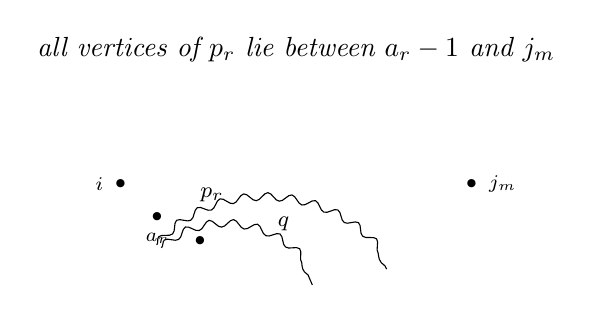
\begin{tikzpicture}[baseline=(current bounding box.east)]
\begin{scope}
	\drawWLDfragment[9]{3}{0.3} % draw arc
	%\drawnumbers % use this to debug
	% highlight region
	%\centerarc[linehighlight](0,0)(\zero + 3.6*\step:\zero + 5.4*\step:\radius)
	% region label
	%\node[align = center] at (\zero + 4.5*\step:\radius*1.3) {\em \footnotesize 0, 1, or 2 vertices \\[3pt]\em \footnotesize in this region};
	% scope to draw props and their labels
	\begin{scope}
		\clipcenterarc(0,0)(\startpoint-20:\endpoint+20:\radius)
		%p_r
		\draw[smallpropagator] (\zero+2.3*\step:\radius*1.1) to [bend left = 55] (\zero + 6.7*\step:\radius*1.1); 
		%q
		\draw[smallpropagator] (\zero+2.4*\step:\radius*1.1) to [bend left = 55] (\zero + 5.3*\step:\radius*1.1); 
		%\draw[smallpropagator,light-gray] (\zero+7.5*\step:\radius*1.1) -- (0:\radius*0.25);  
		\node at (\zero + 2.8*\step:\radius*0.8){\footnotesize $p_r$};
		\node at (\zero + 4.7*\step:\radius*.84){\footnotesize $q$};
	\end{scope}
	% draw nodes
	\newnode[left]{1}{i}
	\newnode[below]{2}{a_r}
	\newnode[below]{3}{}
	\newnode[right]{9}{j_m}
	% case label
	\node at (270:\radius*0.1) {\em all vertices of $p_r$ lie between $a_r-1$ and $j_m$};
\end{scope}
\end{tikzpicture} \qquad \qquad 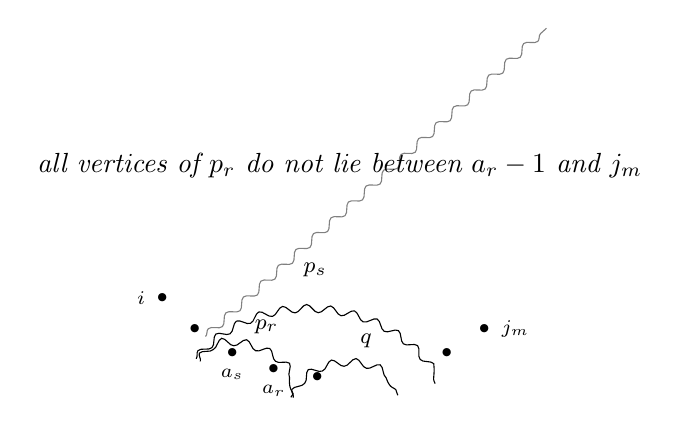
\begin{tikzpicture}[baseline=(current bounding box.east)]
\begin{scope}
	\drawWLDfragment[10]{3}{0.3} % draw arc
	%\drawnumbers % use this to debug
	% highlight region
		% scope to draw props and their labels
	\begin{scope}
		\clipcenterarc(0,0)(\startpoint-20:\endpoint+20:\radius)
		%random prop preventing p_s from contributing a_s-1
		\draw[smallpropagator,gray] (\zero+2.3*\step:\radius) -- (\zero + 16.5*\step:\radius) ;
		%p_s
		\draw[smallpropagator] (\zero+2.4*\step:\radius*1.1) to [bend left = 55] (\zero + 7.5*\step:\radius*1.1); 
		%p_r
		\draw[smallpropagator] (\zero+2.5*\step:\radius*1.1) to [bend left = 90] (\zero + 4.5*\step:\radius*1.1); 
		%q
		\draw[smallpropagator] (\zero+4.55*\step:\radius*1.1) to [bend left = 70] (\zero + 6.7*\step:\radius*1.1); 
		\node at (\zero + 4.5*\step:\radius*0.55){\footnotesize $p_s$};
		\node at (\zero + 3.5*\step:\radius*0.84){\footnotesize $p_r$};
		\node at (\zero + 6.2*\step:\radius*0.85){\footnotesize $q$};
	\end{scope}
	% draw nodes
	\newnode[left]{1}{i}
	\newnode[below]{2}{}
	\newnode[below]{3}{a_s}
	\newnode[below]{4}{a_r}
	\newnode[below]{5}{}
	\newnode[below]{8}{}
	\newnode[right]{9}{j_m}
	% case label
	\node at (270:\radius*0.1) {\em all vertices of $p_r$ do not lie between $a_r-1$ and $j_m$};
\end{scope} 
\end{tikzpicture} }\eas
\caption{The two cases of the induction step. Note that $I_i(p_s) <_i I_i(p_r)$}\label{fig:awkward induction step}
\end{figure}
Now repeat the argument above with $p_s$ in place of $p_r$: if the other end of $p_s$ lands on an edge between $q$ and $j_m$ then we have $q \in \cP_{m-1}$ as above; if not then there exists some $p_t \in Q_{l-3}$ with $p_s$ supported on $I_i(p_t)$ and $q$ on the inside of $p_t$ in the $a_t-1$ order. Therefore $I_i(p_t) <_i I_i(p_r)$
%{\color{violet} May not be necessary, but I think highlighted tex follows from "Now repeat the argument...." \begin{enumerate}\item If $V(p_r) \in [a_r-1, j_m]$ (other end closer to $j_m$) then $q$ inside $p_r$ in $a_r-1$ order. \item Else, $V(p_r) \in [i, a_r+1]$ (Maybe $[i-1, a_r +1]$?). (Main point is that other end closer to $i$) Either way,  admissibility implies that $a_s < a_r$ \item Now we repeat. Either  $V(p_s) \in [a_s-1, j_m]$ then $q$ inside $p_s$ in $a_s-1$ order \hlfix{and we are done}{not quite true; same reasoning as why we're using ``the other end of the propagator'' instead of $V(p_s) \subseteq [a_s-1, j_m]$} \item Else, $V(p_s) \in [i, a_s+1]$ (Maybe $[i-1, a_s +1]$?). Either way, admissibility implies that $a_t < a_s$ and we've already established $a_s < a_r$ \end{enumerate} We don't have to include this argument. It may be totally unnecessary. But I want to make certain that I'm not missing anything.}
Since there are finitely many steps this process can take before reaching $Q_0$, and any $p_* \in Q_0  = \Prop(j_m)$ has $j_m$ in its support by definition, this argument eventually terminates with the construction of a propagator constraining the positioning of $q$ as required. This completes the induction step, and hence the proof.\end{proof}



We have now shown that Algorithm~\ref{alg:put GN on WLD} associates the correct Grassmann necklace to a Wilson loop diagam. Therefore, we refer to Algorithm~\ref{alg:put GN on WLD} as the Grassmann necklace algorithm. We close this section with a simple observation about the Grassmann necklaces of positroids associated to Wilson loop diagrams.


In an arbitrary Grassmann necklace, it is possible for an index $i$ to appear in no terms of the Grassmann necklace (a {\em loop}) or in all terms of the necklace (a {\em coloop}). Using Theorems~\ref{res:alg gives GN} and \ref{res alg gives correct GN}, a characterization of the loops and coloops of the Grassmann necklace associated to a Wilson loop diagram follows easily.


\begin{cor}\label{no coloops}
Grassmann necklaces coming from admissible Wilson loop diagrams have no coloops. A vertex $j$ is a loop if and only if $j$ supports no propagators. 
\end{cor}
\begin{proof}
For any $i \in [n]$, $i-1$ is maximal with respect to the $<_{i}$ order and so by Lemma~\ref{lem no fourth vertex} there can be no propagator $p$ with $I_{i}(p) = i-1$. Thus $i-1 \not\in I_{i}$, so $i-1$ is not a coloop. Since this holds for any $i \in [n]$, the Grassmann necklace admits no coloops.

If $j \in [n]$ is a loop then in particular we have $j \not\in I_j$, which can only happen if there are no propagators supported on vertex $j$. Conversely, if $j$ supports no propagators, then Algorithm~\ref{alg:put GN on WLD} never assigns a propagator to $j$ and hence $j \not\in I_i$ for all $i \in [n]$.
\end{proof}





\section{Dimension of the Wilson Loop cells}\label{sec dim}

In continuing to characterise the poistroid cells associated to Wilson loop diagrams, our next goal is to show that the dimension of the positroid cell defined by a Wilson loop diagram $(\cP, [n])$ has dimension $3|\cP|$ (Theorem \ref{thm dim}).  The positroid cells associated to the Amplituhedron are of dimension $4|\cP|$. In \cite{non-orientable}, Agarwala and Marcott show that the dimension of the Deodhar component is the sum of $|\cP|$ and the dimension of the associated positroid cell.
%\[|\cP| + \text{ the dimension of associated positroid cell}.\]
In other words, the Deodhar component associated to a Wilson loop diagram is $4|\cP|$, showing that the geometry underlying the Wilson loop diagrams is consistent with the geometry underlying the Amplituhedron.

Marcott in \cite{WLDdim} gives a different proof of the $3|\cP|$-dimensionality of $M(W)$ which is geometric and more elegant, but it is not easy to track the effect of a particular propagator.  Our approach is much more explicit.

Recall that the dimension of a positroid cell is equal to the number of plusses in the associated Le diagram \cite[Theorem 6.5]{Postnikov}. By combining Algorithms~\ref{alg:put GN on WLD} and \ref{alg:GN to Le} (converting from WLD to Grassmann necklace, and Grassmann necklace to Le diagram respectively) we explicitly describe the effect of adding another propagator to a Wilson loop diagram in terms of the plusses of the associated Le diagrams, and hence give a recursive proof of the $3|\cP|$-dimensionality of the cells.

More than just a dimensionality result, the lemmas below are a first step towards undertanding how the adding an extra propagator changes the associated positroid cell. 

We start with several lemmas, of roughly increasing degree of technicality. We begin by relating non-supporting vertices to columns of zeros in the Le diagram (Lemma \ref{lem uncovered}) and verifying that performing dihedral transformations on a Wilson loop diagram does not change the dimension of of the associated Le diagram (Lemma \ref{lem dihedral}).

\begin{lem}\label{lem uncovered}
Let $W$ be an admissible Wilson loop diagram with $k$ propagators, and with a vertex $i$ that supports no propagators.  Let $V$ be $W$ with vertex $i$ removed.  Then the Le diagram of $W$ is obtained from the Le diagram of $V$ by inserting an extra column containing all $0$s in position $i$ (i.e. such that the new column has the label $i$).
\end{lem} 

\begin{proof}
  By Algorithm~\ref{alg:put GN on WLD} the Grassmann necklace of $W$ is obtained from the Grassmann necklace of $V$ by duplicating the $i$th element of the Grassmann necklace of $V$, and incrementing all indices greater than $i$ by $1$ in each Grassmann necklace element.  Formally, 
  \[
  I_j^{W} =
  \begin{cases}
    \{\ell \in I_j^{V} : \ell < i\} \cup \{\ell+1 \in I_j^{V} : \ell \geq i\} & \text{if $j\leq i$} \\
    \{\ell \in I_{j-1}^{V} : \ell < i\} \cup \{\ell+1 \in I_{j-1}^{V} : \ell \geq i\} & \text{if $j > i$.}
  \end{cases}
  \]


By Corrollary~\ref{no coloops} we know that $i \not\in I_1^W$, and so $i$ must label a horizontal edge on the boundary of the Le diagram of $W$, i.e. it must be a column label. The shapes of the Le diagram of $V$ and $W$ are the same except for the insertion of this column since $I_1$ is the same for $V$ and $W$ except for the incrementation of the indices $\geq i$ in the transition from the necklace for $V$ to the necklace for $W$. 
\end{proof}


\begin{lem}\label{lem dihedral}
If two Wilson loop diagrams differ by a dihedral transformation then their Le diagrams have same number of plusses.
\end{lem}
\begin{proof}
By \cite[Proposition 17.10]{Postnikov}, the dimension of a positroid (and hence the number of plusses in its Le diagram) is $k(n-k) - A(\pi_W)$, where $A(\pi_W)$ denotes the number of alignments of the decorated permutation $\pi_W$ of the positroid associated to $W$. (See \cite[Figure 17.1]{Postnikov} and preceding discussion.)

It can easily be seen from \cite[Section 17]{Postnikov} and Algorithm \ref{alg:put GN on WLD} that dihedral transformations of a Wilson loop diagram $W$ correspond to dihedral transformations of the chord diagram representation of $\pi_W$. Since the number of alignments in a chord diagram is preserved under dihedral transformations, the result follows.
\end{proof}


\begin{lem}\label{lem good p}
  Let $W$ be an admissible Wilson loop diagram with $k \geq 1$ propagators.  Then there is some dihedral transformation of $W$ such that the resulting diagram $W'$ has a propagator $p$ with the following properties:
  \begin{itemize}
  \item $p = (i, n-1)$ for some $i$, and $p$ has no propagators inside it w.r.t the $<_i$ ordering.
  \item Either the edge $i$ in $W'$ only supports $p$, or the edge $i$ in $W'$ supports exactly one other propagator $q = (j,i)$, with no other propagators inside $q$ in the $<_j$ ordering. 
  \end{itemize}
\end{lem}
Note that since the first condition tells us that $p$ has nothing inside it, if $q$ exists in the second condition then $j<_ji<_jn-1$. 

\begin{proof}
  Remove all vertices of $W$ which do not support any propagators to get a weakly admissible Wilson loop diagram $V$.  Lemma~\ref{lem sian} applied to $V$ gives a length 2 propagator $p$ in $V$ for which either no other propagator is supported on one of the supporting edges of $p$ or there is a second length 2 propagator which is the only other propagator supported on one of the supporting edges of $p$.  (Figure~\ref{fig 3 cases} shows the possible configurations arising from Lemma~\ref{lem sian}, and the reader can easily check that in each case $p$ must be in one of the two situations described above.)

  We can now make a dihedral transformation of $V$ to obtain a diagram satisfying the statement of the lemma with $p$ and $q$ both length 2. Restoring the vertices which do not support any propagators, we obtain a dihedral transformation $W'$ of $W$ as desired (with potentially longer lengths for $p$ and $q$).
\end{proof}



Combining Lemmas \ref{lem uncovered}, \ref{lem dihedral}, and \ref{lem good p}, it therefore suffices to study the Le diagrams of weakly admissible Wilson loop diagrams with no non-supporting vertices and admitting one of the configurations described in Lemma \ref{lem good p}, with propagators $p = (n-3, n-1)$ and $q= (n-5, n-3)$ (if $q$ exists) both of length 2. See Figure~\ref{fig special p} for an illustration of the two possibilities. 

With the above restrictions in place, the next few lemmas describe how the Grassmann necklaces (Lemma \ref{lem I}) and the Le diagrams (Lemmas \ref{lem shape} to Lemma \ref{lem other k}) change upon the removal of $p$ from the Wilson loop diagram.  This gives us the inductive lever we need to prove the main theorem (Theorem \ref{thm dim}).


\begin{figure}
\[
\begin{tikzpicture}[rotate = 150,baseline=(current bounding box.east),label distance = -2mm]
\begin{scope}
  \drawWLDfragment[6]{3}{0.3}
  %\drawnumbers % use this to debug
  \begin{scope}
    \clipcenterarc(0,0)(\startpoint:\endpoint:\radius)
    \draw[smallpropagator] (\zero+2.4*\step:\radius*1.1) to [bend left = 55] (\zero + 4.6*\step:\radius*1.1); 
    \node at (\zero + 3.5*\step:\radius*0.75){\footnotesize $p$};
  \end{scope}
  \centerarc[red,line width = 2pt,line cap = round](0,0)(\zero + 2*\step:\zero+4.45*\step:\radius)
  \newbetternode[{[label distance=-3mm]above right}]{1}{n-4}
  \newbetternode[{[label distance=-3mm]above right}]{2}{n-3}
  \newbetternode[{[label distance=-3mm]above right}]{3}{n-2}
  \newbetternode[{[label distance=-3mm]above right}]{4}{n-1}
  \newnode[above]{5}{n}
  \newnode[above]{6}{1}
  \node at (180-60:\radius*0.1){\em Case 1};
\end{scope}
\end{tikzpicture}
\qquad 
\qquad 
\begin{tikzpicture}[rotate=150, baseline=(current bounding box.east)]
\begin{scope}
  \drawWLDfragment[7]{3}{0.3}
  %\drawnumbers % use this to debug
  \begin{scope}
    \clipcenterarc(0,0)(\startpoint:\endpoint:\radius)
    \draw[smallpropagator] (\zero+1.4*\step:\radius*1.1) to [bend left = 60] (\zero + 3.5*\step:\radius*1.1); 
    \draw[smallpropagator] (\zero+3.5*\step:\radius*1.1) to [bend left = 60] (\zero + 5.6*\step:\radius*1.1); 
    \node at (\zero + 2.4*\step:\radius*0.8){\footnotesize $q$};
    \node at (\zero + 4.5*\step:\radius*0.8){\footnotesize $p$};
  \end{scope}
  \centerarc[red,line width = 2pt,line cap = round](0,0)(\zero + 1.6*\step:\zero+5.5*\step:\radius)
  \newbetternode[{[label distance=-3mm]above right}]{1}{n-5}
  \newbetternode[{[label distance=-3mm]above right}]{2}{n-4}
  \newbetternode[{[label distance=-3mm]above right}]{3}{n-3}
  \newbetternode[{[label distance=-3mm]above right}]{4}{n-2}
  \newbetternode[{[label distance=-3mm]above right}]{5}{n-1}
  \newnode[above]{6}{n}
  \newnode[above]{7}{1}
  \node at (180-60:\radius*0.1){\em Case 2};
\end{scope}
\end{tikzpicture}
\] 
  \caption{The two cases for $W$ and $p$.  No other propagators can end in the red sections.  Other segments may have additional propagators ending in them.}\label{fig special p}

\end{figure}


\begin{lem}\label{lem I}
Let $W$ be an admissible Wilson loop diagram with $k\geq 1$ propagators, and suppose that $W$ admits one of the configurations described in Lemma~\ref{lem good p}, with $p$ and $q$ (if $q$ exists) both of length 2. Let $V$ be $W$ with $p$ removed.  Then we can express $I_*^W$ in terms of $I_*^V$ as follows:

  \begin{align*}
    I_1^{W} & = I_1^{V} \cup \{n-3\} \\
    I_n^{W} & = I_1^{V} \cup \{n\} \\
    I_{n-1}^{W} & = I_n^{V} \cup \{n-1\} \\
    I_{n-2}^{W} & =
    \begin{cases}
      I_{n-2}^{V}\cup \{n-2\} & \text{if $n-2\not\in I_{n-2}^{V}$} \\
      I_{n-2}^{V}\cup \{n-1\} & \text{if $n-2\in I_{n-2}^{V}$, $n-1\not\in I_{n-2}^{V}$} \\
      (I_{n}^{V} \setminus \{n-5\})\cup \{n-1,n-2\} & \text{if $n-1, n-2\in I_{n-2}^{V}$}
    \end{cases} \\
    I_{k}^{W} & =
    \begin{cases}
      I_k^{V}\cup \{n-3\} & \qquad \qquad \qquad \qquad \text{if $n-3 \not\in I_k^{V}$}\\
      I_k^{V}\cup\{n-2\} & \qquad \qquad \qquad \qquad \text{if $n-3\in I_k^{V}$}
    \end{cases} \\
    & \text{for $1<k<n-2$}
  \end{align*}
\end{lem}


\begin{proof}
The two possible cases for $W$ are illustrated in Figure~\ref{fig special p}. 

We begin with $I_1$, and first observe that by Remark~\ref{rmk cyclic} we must have $I_1^W(p) = n-3$. Since $p$ is the final propagator to be assigned by $I_1^W$, it follows that $I_1^W$ and $I_1^V$ behaved identically on all earlier propagators (recall Remark~\ref{rmk algorithm locally same} about locally identical propagator configurations), which implies in particular that $n-3 \not\in I_1^V$. Thus $I_1^W = I_1^V\cup\{n-3\}$.

We note for future reference that the arguments of the previous two paragraphs also imply that $n-2,n-1,n \not\in I_1^V$.

Next consider $I_n^{W}$. From the figure we see that in both cases we have $I_n^{W}(p) = n$.  At vertex 1 of the algorithm $I_n$, the unassigned propagators are exactly those that appear in $V$. Therefore the algorithm continues as in $I_1^{V}$, i.e. we have $I_n^{W} = I_1^{V} \cup \{n\}$. By a similar argument, we must have $I_{n-1}^{W} = I_n^{V} \cup \{n-1\}$.

Now consider $I_{n-2}^{W}$. If $n-2\not\in I_{n-2}^{V}$ then the vertex $n-2$ is non-supporting (see also Corrollary~\ref{no coloops}.)  Thus we are in Case 1, with ${I_{n-2}^W(p) = n-2}$ and this assignment of $p$ does not affect the rest of the construction of $I_{n-2}^{V}$, so we obtain ${I_{n-2}^{W} = I_{n-2}^{V}\cup \{n-2\}}$ as above.

On the other hand, if $n-2\in I_{n-2}^{V}$ then we must be in Case 2 of Figure~\ref{fig special p} and $I_{n-2}^V(q) = I_{n-2}^W(q) = n-2$ (since $q$ is always the clockwise-most propagator supported on vertex $n-2$. If $n-1 \not\in I_{n-2}^{V}$, then $I_{n-2}^W(p) = n-1$ and then the algorithm proceeds identically to $I_{n-2}^{V}$ for the remainder of its steps; thus $I_{n-2}^{W} = I_{n-2}^{V}\cup \{n-1\}$ in this case.

Finally, if $n-2,n-1 \in I_{n-2}^{V}$ then $I_{n-2}^W(q) = n-2$ and $I_{n-2}^W(p) = n-1$ as above, but but some other propagator must have contributed $n-1$ to $I_{n-2}^{V}$ so we cannot use the same argument as above. When the algorithm $I_{n-2}^W$ reaches vertex $n$, only the propagators $p$ and $q$ have contributed; thus we proceed as in the construction of $I_n^{V}$ but without propagator $q$ by Remark \ref{rmk algorithm locally same}. By Lemma~\ref{vertex cyclic int lem} we know that $I_n^V(q) = n-5$, and from Remark \ref{clockwise ordering rem} we see that the only way this could occur is if $q$ was the last to contribute to $I_{n-2}^V$. %all other propagators in $V$ had already been assigned when we reached vertex $n-5$; thus $q$ was the final propagator contributing to $I_n^{V}$. 
Therefore $I_{n-2}^{W} = (I_{n}^{V} \setminus \{n-5\}) \cup \{n-1, n-2\}$ in this case. This completes all cases for $I_{n-2}^{W}$.

The arguments for $I_k^{W}$ ($1< k < n-2$) proceed analagously to those of $I_{n-2}^{W}$, with one simplification: we cannot have both $n-3$ and $n-2$ in $I_k^{V}$ since $q$ is the only propagator that could be assigned to either of them, and it cannot be assigned to both.

This covers all cases and hence completes the proof.
\end{proof}

The next several lemmas assume $V$ and $W$ to be as above. They discuss how the shape of the Le diagram changes from $V$ to $W$ and how the plusses in $V$ shift to become plusses in $W$. In particular, the Le diagram for $W$ has an extra row, labeled by $n-3$, with three columns (see Figure~\ref{fig Le} and Lemma~\ref{lem shape}). This last row contains three (new) plusses. All other plusses in the Le diagram of $V$ shift in a predictable manner to become plusses in the Le diagram of $W$; this is described in Lemmas~\ref{lem n and n-1} to Theorem~\ref{thm dim}.

We proceed to address the cases laid out in Lemma~\ref{lem I}, getting the shape of the Le diagram of $W$ from the relation $I_1^W= I_1^V \cup \{n-3\}$. 

\begin{lem}\label{lem shape}
  Let $V$ and $W$ be as in Lemma~\ref{lem I}.
  The shape of the Le diagram of $V$ can be built from left to right of the following blocks: a rectangle which is 3 columns wide, one more column of the same height, and a partition shape with at most as many rows as the rectangle.
  The shape of the Le diagram of $W$ can be built from left to right of the following blocks: a rectangle with 3 columns and one more row than the first rectangle of $V$, and the same partition shape as in $V$.
\end{lem}

\begin{proof}
See Figure~\ref{fig Le} for an illustration of the shapes described in the statement of the lemma.

Recall that $I_1$ determines the shape of the Le diagram: specifically, the elements of $I_1$ label the rows of the diagram, working from top right to bottom left. By the arguments in Lemma {\ref{lem I}} we know that ${n,n-1,n-2, n-3 \not\in I_1^{V}}$.  These are the leftmost four columns of the diagram for $V$.  From Lemma \ref{lem I} we know that that $I_1^{W} = I_1^{V}\cup \{n-3\}$. Therefore, the right hand boundary of the shape of $V$ is the same as the right hand boundary of the shape of $W$ except that $W$ has one additional row of 3 boxes while $V$ has an additional column in the $n-3$ position; that is, an extra column fourth from the left. 
\end{proof}
\begin{figure}
  \[\begin{tikzpicture}[scale = 1.5]
\node at (1.5,2.5) {\Large $V$};
\draw (0,0) rectangle (1,2);
\draw (1,0) rectangle (1.3,2);
\begin{scope}[shift = {(-2.7,-2)}]
\draw (4,2) .. controls (5.3,2.2) and (4.7,3) .. (5.5,3.2) .. controls (6.3,3.5) .. (6.5,4) -- (4,4);
\end{scope}
\node at (0.5,1) {\large$\mathcal{A}$};
\node at (1.8,1) {\large$\mathcal{B}$};
\begin{scope}[shift = {(5,0)}]
\node at (1.5,2.5) {\Large $W$};
\draw (0,-0.3) rectangle (1,0);
\draw (0,0) rectangle (1,2);
\begin{scope}[shift = {(-3,-2)}]
\draw (4,2) .. controls (5.3,2.2) and (4.7,3) .. (5.5,3.2) .. controls (6.3,3.5) .. (6.5,4) -- (4,4);
\end{scope}
\node at (0.5,1) {\large$\mathcal{A}$};
\node at (1.5,1) {\large$\mathcal{B}$};
\end{scope}
\end{tikzpicture}\]
  \caption{Le diagrams for $V$ (left) and $W$ (right).}\label{fig Le}
\end{figure}

As illustrated in Figure~\ref{fig Le}, the pieces of the Le diagrams of $V$ and $W$ will be called $\mathcal{A}$ and $\mathcal{B}$ in what follows. Explicitly, $\mathcal{B}$ is the set of columns with labels $v < n-3$ and $\mathcal{A}$ is the set of columns labeled by $n$, $n-1$ and $n-2$ in $V$. In $W$ we see that $\mathcal{A}$ consists of these columns without the last row. Over the course of the next few lemmas we will prove that the plusses in the $\mathcal{B}$ parts of each diagram are identical, and that the relationship between the plusses in the two $\mathcal{A}$ regions can be described explicitly.

We do this by applying Algorithm~\ref{alg:GN to Le}, which constructs the Le diagram associated to a Grassmann necklace, to the Grassmann necklaces of $V$ and $W$. As described in Section~\ref{sec:positroid background}, if Algorithm~\ref{alg:GN to Le} places a $+$ in the box with row index $i$ and column index $j$, we say that this plus is {\bf in the $i \rightarrow j$ position}, and refer to it as {\bf the plus defined by ``the (hook) path from $i$ to $j$''}. Note that the collection of paths contributed by a single Grassmann necklace term must be non-crossing: this follows immediately from the Le condition.

Finally, we also note that when we speak of a plus in the Le diagram of $V$ being the same as in $W$ or vice versa, we mean that the position of the plus in $\mathcal{A}$ or $\mathcal{B}$ is the same.




\begin{lem}\label{lem n and n-1}
Let $V$ and $W$ be as in Lemma~\ref{lem I}.
Then
  %$I_n^{W}$
  %and $I_{n-1}^{W}$ together yield the same plusses as $I_n^{V}$ did, along with two extra plusses which appear in the leftmost two boxes of the bottom row of the Le diagram of $W$.
%
%  Specifically,
  $I_n^W$ yields an $(n-3)\rightarrow n$ plus and $I_{n-1}^W$ yields an $(n-3)\rightarrow (n-1)$ plus along with any plusses yielded by $I_n^V$.
\end{lem}

\begin{proof}
By Lemma~\ref{lem I} we have $I_n^{W}= I_1^{V} \cup \{n\}$ and $I_1^{W} = I_1^{V} \cup \{n-3\}$. Thus 
\[I_1^{W} \setminus I_n^{W} = \{n-3\}, \qquad \qquad I_n^{W} \setminus I_1^{W} = \{n\},\]
and so by Algorithm~\ref{alg:GN to Le} we have a plus in the $(n-3) \rightarrow n$ position, i.e. in the leftmost box of the bottom row. 

Also by Lemma~\ref{lem I} we have $I_{n-1}^{W} = I_n^{V} \cup \{n-1\}$. Recall from the proof of Lemma~\ref{lem I} that $n-3,n-2,n-1,n \not\in I_1^V$; therefore
\[
I_1^W\setminus I_{n-1}^W = (I_1^V \setminus I_n^V) \cup\{n-3\},
\]
and $n-3$ is maximal in this set. Similarly, 
\[I_{n-1}^W \setminus I_1^W = (I_n^V \setminus I_1^V) \cup \{n-1\}.
\]
Also $(I_n^V \setminus I_1^V) \cup \{n-1\}\subseteq \{n-1,n\}$ from the definition of Grassmann necklace and so in particular, $n-1$ is minimal in this set, so Algorithm~\ref{alg:GN to Le} yields a plus in the $(n-3) \rightarrow (n-1)$ position (i.e. the second box in the bottom row of the Le diagram of $W$) along with any plusses yielded by $I_n^V$.
\end{proof} 

In the next two lemmas, we consider the plusses contributed to the Le diagram of $W$ by $I_{n-2}^W$. Lemma~\ref{lem I} lists three possibilities for $I_{n-2}^W$, but the following observation shows that we need only consider two of them.

\begin{rmk}\label{rem n-2 case} Consider the case when $n-2 \in I_{n-2}^V$ but $n-1 \not\in I_{n-2}^V$. This case can only occur if our $W$ is in Case 2 of Figure~\ref{fig special p} and $n-1$ supports no propagators other than $p$. In this situation, apply the dihedral transformation that reflects $W$ along the line perpendicular to the $(n-2)^{th}$ edge, so that $p$ is unchanged but $q = (n-1,1)$ in the new diagram. The new diagram is an example of Case 1, i.e. satisfying $n-2 \not \in I_{n-2}^V$. Therefore we do not need to consider the case where $n-2\in I_{n-2}^V$ but $n-1\not\in I_{n-2}^V$.
\end{rmk}

\begin{lem}\label{lem n-2 good}
  Let $V$ and $W$ be as in Lemma~\ref{lem I}, and suppose that $n-2 \not\in I_{n-2}^{V}$. Then $I_{n-2}^{W}$ contributes all of the same plusses as $I_{n-1}^{V}$ (which is the same as $I_{n-2}^{V}$) along with a new $(n-3)\rightarrow (n-2)$ plus.
\end{lem}


\begin{proof}
If $n-2\not\in I_{n-2}^{V}$ then $I_{n-1}^{V}=I_{n-2}^{V}$ by definition, and by Lemma~\ref{lem I} we have the equality ${I_{n-2}^{W} = I_{n-1}^{V} \cup \{n-2\}}$.  Note that $n-3\not\in I_{n-2}^{V}$ by Lemma~\ref{lem no fourth vertex}.  Therefore the plusses contributed by $I_{n-2}^{W}$ are exactly the  plusses from $I_{n-1}^{V}$ along with the $(n-3)\rightarrow (n-2)$ plus.  This gives the statement of the lemma.
\end{proof}

Next we need an observation about how the Grassman necklace for $V$ changes over the indices near $n$ under the hypotheses that $n-2, n-1\in I_{n-2}^V$.

Specifically with $V$ and $W$ as in Lemma~\ref{lem I} and with $n-2, n-1\in I_{n-2}^V$ (so we are necessarily in Case 2 and $n-1$ supports at least one additional propagator) we have
  \begin{equation}\label{eq necklace}
  I_{n-3}^{V} \xrightarrow[\substack{n-3\text{ out}\\n-2\text{ in}}]{} I_{n-2}^{V} \xrightarrow[\substack{n-2\text{ out}\\n-5\text{ in}}]{} I_{n-1}^{V} \xrightarrow[\substack{n-1\text{ out}\\ u \text{ in}}]{} I_{n}^{V}  \xrightarrow[\substack{n \text{ out}\\v \text{ in}}]{} I_1^{V}
  \end{equation}
where $u$ and $v$ are two vertices; we will derive some properties of them below.

The first two transitions follow by the cyclic intervals property highlighted in Remark~\ref{rmk cyclic} along with the fact that $n-3$ is a supporting vertex in $V$.  The third transition follows from the definition of Grassmann necklaces and the fact that $n-1\in I_{n-2}^V$ by hypothesis, while the final transition follows from the fact that $n-1$ supports an additional propagator so we are guaranteed $n \in I_n^V$.

Note that neither $u$ nor $v$ can be $n-1$, $n-2$, or $n-3$, because, as noted in Lemma~\ref{lem I}, these elements do not belong to $I_1^V$ and $I_n^V = (I_1^V\setminus \{v\}) \cup \{n\}$. However, $u$ could be $n$.  

Also $u$ cannot be $n-4$, for the following reason. By Remark~\ref{rmk cyclic} we know that $I_{n-1}^W(q) = n-5$, leaving no propagators supported on $n-4$ for $I_{n-1}^W$ to assign. Thus $n-4 \not\in I_{n-1}^W$. Since $I_{n-1}^W = I_n^V\cup\{n-1\}$ by Lemma~\ref{lem I}, we cannot have $n-4$ in $I_n^V$ either.

However, it is important to observe that $v$ could be $n-4$, as we see in the next result. 


  \begin{lem}\label{lem n-2 bad}
    Let $V$ and $W$ be as in Lemma~\ref{lem I}, and suppose that $n-2,n-1 \in I_{n-2}^{V}$. Let $c$ be the largest element of $I_1^V$.  Then the following are true.
    \begin{enumerate}
  \item $c=n-4$ if $n-4\in I_1^V\setminus I_n^V$ and $c=n-5$ otherwise. If $c = n-4$ then we have $v = n-4$ in equation \eqref{eq necklace}.
  \item $I_{n-3}^W$ contributes the same plusses as $I_{n-3}^V$, except that the plus in the $n-3$ column (which necessarily exists) is shifted one square left into the $n-2$ column.
  \item In the Le diagram of $V$, $I_{n-2}^{V}$ contributes a $(c)\rightarrow (n-2)$ plus and no other term in the Grassmann necklace of $V$ gives a plus in this column. All other plusses from $I_{n-2}^{V}$ were already contributed by $I_{n-3}^V$.
  \item $I_{n-2}^W$ contributes an $(n-3) \rightarrow (n-2)$ plus, a $(c) \rightarrow (n-1)$ plus, and one other plus. If $c = n-5$ then this third plus is the one contributed by $I_n^V$, while if $c = n-4$ then the third plus is $(n-5) \rightarrow n$.
  \item If $c = n-4$ then $I_{n-1}^V$ contributes a $(n-4) \rightarrow (n-1)$ plus; all other plusses contributed by $I_{n-1}^V$ were already contributed by $I_{n-3}^V$, regardless of the value of $c$.
  \item The Grassmann necklace of $V$ contributes a $(c)\rightarrow (n-1)$ plus if and only if $c = n-4$. No term in the Grassmann necklace of $V$ contributes a $(n-5) \rightarrow n$ plus.
    \end{enumerate} 
\end{lem}

\begin{proof}
\begin{enumerate}  

\item As in Lemma~\ref{lem I} we have $n,n-1,n-2,n-3 \not\in I_1^V$, which implies the first part of the claim. The second part is a consequence of the discussion following \eqref{eq necklace}, which shows that $n-4 \not\in I_n^V$.

\item By Lemma~\ref{lem I} we have that $I_{n-3}^W = I_{n-3}^V \cup \{n-2\}$, so $I_{1}^W \setminus I_{n-3}^W = I_1^V \setminus I_{n-3}^V$ and $I_{n-3}^W \setminus I_1^W$ is obtained from $I_{n-3}^V \setminus I_{1}^V$ by replacing the $n-3$ with $n-2$.    

\item From equation \eqref{eq necklace} the pair of sets $(I_{n-2}^V\setminus I_1^V, I_1^V\setminus I_{n-2}^V)$ is either $(\{n-2, n-1, n\}, \{n-5, u, v\})$ (if $n \in I_{n-2}^V$) or $(\{n-2, n-1\}, \{n-5, v\})$ (if $n \not\in I_{n-2}^V$, i.e. $u = n$).

Recall that we cannot have $u = n-4$ (since $n-4 \notin I_n^V$) so either $u = n$ or $u < n-5$, and either way $n-2$ is minimal in $I_{n-2}^V\setminus I_1^V$ and $c$ is maximal in $I_1^V \setminus I_{n-2}^V$, yielding a $(c) \rightarrow (n-2)$ plus. 

Since $I_{n-2}^V$ is the only term in the Grassmann necklace for $V$ that contains $n-2$, no other term can contribute a plus in column $n-2$. Additionally, since $I_{n-2}^V$ only differs from $I_{n-3}^V$ in that the $n-3$ was replaced by an $n-2$, all other plusses must agree with those contributed by $I_{n-3}^V$. 

\item By Lemma~\ref{lem I} we have $I_1^W = I_1^V\cup \{n-3\}$ and $I_{n-2}^W = (I_n^V \setminus \{n-5\}) \cup \{n-1,n-2\}$. By equation \eqref{eq necklace} we have $n-5 \in I_1^V$, and by the following discussion we have $n-1,n-2,n-3 \not\in I_n^V,I_1^V$. It follows that the symmetric difference of $I_1^W$ and $I_{n-2}^W$ is
    \begin{gather*}
    I_1^W \setminus I_{n-2}^W  = (I_1^V\setminus I_n^V) \cup \{n-3, n-5\}. \\
    I_{n-2}^W \setminus I_1^W  = (I_n^V\setminus I_1^V) \cup \{n-1, n-2\}.
\end{gather*}
As per the discussion following equation \eqref{eq necklace} above, we also have $I_n^V\setminus I_1^V = \{n\}$ and $I_1^V\setminus I_n^V = \{v\}$. If $c = n-5$ then the path $v \rightarrow n$ from $I_n^V$ does not intersect with the paths from $\{n-3, n-5\}$ to $\{n-2, n-1\}$ and we obtain the plusses as stated.
    
Now suppose $c = v= n-4$; in this case $I_{n-2}^W$ contributes plusses defined by the noncrossing paths starting from $\{n-3, n-4, n-5\}$ and ending at $\{n, n-1, n-2\}$, namely the plusses in positions $(n-3)\rightarrow (n-2)$, $(n-4)\rightarrow (n-1)$ and $(n-5)\rightarrow (n)$.

\item Combining equation \eqref{eq necklace} with point 3 of this proof, the pair $(I_{n-1}^V \setminus I_1^V, I_1^V \setminus I_{n-1}^V)$ is either $(\{n-1, n\}, \{u, v\})$ or $(\{n-1\}, \{v\})$. Per point 1, $c = n-4$ if and only if $v = n -4$, in which case we get a $(n-4) \rightarrow (n-1)$ plus and the $u \rightarrow n$ plus (if it exists) has already been contributed by $I_{n-2}^V$ and $I_{n-3}^V$. If $c = n-5$ then $v < n-5$ and we are in the same situation as $I_{n-2}^V$. 

\item A Grassmann necklace term $I_i^V$ can only contribute a path beginning at $c$ when $c \not\in I_i^V$. Further, since $c$ will always be maximal in $I_1^V\setminus I_i^V$ by point 1, a path from $c$ must end at the minimal element of $I_i^V \setminus I_1^V$. From \eqref{eq necklace}, the only way we can have $c \not\in I_i^V$ and $n-1$ minimal in $I_i^V \setminus I_1^V$ is if $c = n-4$ and $i = n-1$.

Similarly, the only terms that can contribute an $(n-5) \rightarrow n$ plus are those with $n-5 \in I_i^V$, i.e. when $i \in \{n-2,n-3,n-4\}$. However, $n-5$ is always the largest or second-largest element in $I_1\setminus I_i^V$, while if $n \in I_i^V \setminus I_1^V$ for $i \in \{n-2,n-3,n-4\}$ then $|I_i^V \setminus I_1^V| \geq 3$ and so $n$ cannot be the smallest or second-smallest in this set. Thus there can be no path $(n-5) \rightarrow n$.
\end{enumerate}
\end{proof}


\begin{lem}\label{lem other k}
  Let $V$ and $W$ be as in Lemma~\ref{lem I}, and suppose that if $n-2\in I_{n-2}^{V}$ then $n-1\in I_{n-2}^{V}$ also. Then for each $k$ in the range $1<k<n-2$, $I_k^{W}$ contributes the same plusses as $I_{k}^{V}$, except that if $I_{k}^{V}$ contributed a plus in the $n-3$ column of the Le diagram of $V$ then this plus is shifted one square left in the Le diagram of $W$.
\end{lem}

\begin{proof}
Recall that $I_1^W = I_1^V\cup \{n-3\}$ and that $n-2,n-1,n \not\in I_1^W$.

  If $n-3\not\in I_{k}^{V}$ then by Lemma~\ref{lem I} we have $I_{k}^{W} = I_k^{V}\cup \{n-3\}$.  Then since $n-3$ is the largest element of $I_1^{W}$ this transformation leaves the disjoint paths unchanged and so the plusses carry over from $V$ to $W$ directly.

  If $n-3\in I_{k}^{V}$ then $I_k^V$ must contribute a plus in the $n-3$ column of the Le diagram of $V$, and by Lemma~\ref{lem I} we have $I_{k}^{W} = I_k^{V}\cup \{n-2\}$. If $n-2$ supports no propagators in $V$ then certainly no plusses appear in the $n-2$ column of the Le diagram of $V$. If $n-2$ supports at least one propagator in $V$ then $n-2 \in I_{n-2}^V$ and so by hypothesis $n-1 \in I_{n-2}^V$ as well. By Lemma~\ref{lem n-2 bad} item 3, the only necklace element of $V$ containing $n-2$ is $I_{n-2}^{V}$ and further with item 4, the plusses in column $n-2$ from $I_{n-2}^V$ and $I_{n-2}^W$ are different.

  Since $n-3 \in I_k^V \setminus I_1^V$, we must have a path in the Le diagram of $V$ from some vertical edge $i$ to the bottom edge $n-3$.  In the Le diagram of $W$, the index $n-3$ labels a vertical edge with no path from $I_k^W$ starting at it (since $n-3$ belongs to both $I_1^W$ and $I_k^W$), and there must be a path leading to $n-2$ since $n-2 \in I_k^W \setminus I_1^W$.  By the previous paragraph no other path from $I_k^V$ could end at $n-2$, and since the paths cannot cross we conclude that the $i\rightarrow (n-3)$ path in the Le diagram of $V$ must become a $i\rightarrow (n-2)$ path in the Le diagram of $W$. All other paths are unchanged.

%   Thus the plus contributed by $I_k^V$ in the $n-3$ column of the Le diagram of $V$ is shifted into the $n-2$ column in the Le diagram for $W$, where there was no plus before, and no other plusses are changed.
\end{proof}

We are now ready to prove the main result of this section, showing that the dimension of the positroid cell associated to each Wilson loop diagram is $3|\cP|$. 

\begin{thm}\label{thm dim}
Let $W = (\cP, [n])$ be an admissible Wilson loop diagram.  The number of plusses in the Le diagram of of $W$ is three times the number of propagators.
\end{thm}

\begin{proof}
  The proof is by induction on the number of propagators.

  First note that a Wilson loop diagram $W$ with one propagator supported on vertices $i<i+1<j<j+1$ has a Le diagram consisting of a single row with $n-i$ boxes. The columns are labeled from left to right by $n, \ldots, i+1$. By Algorithm~\ref{alg:GN to Le} there are plusses in the $i+1$, $j$, and $j+1$ positions. 

  Now consider Wilson loop diagrams with $k>1$ propagators.  By Lemma~\ref{lem uncovered} it suffices to prove the result for weakly admissible Wilson loop diagrams with $k$ propagators and no non-supporting vertices.  By Lemma~\ref{lem dihedral} it suffices to prove the result for at least one Wilson loop diagram from each dihedral orbit. In particular, we can restrict our attention to diagrams $W$ which have a propagator $p$ with the properties in Lemma~\ref{lem good p}.  

%We make one further simplification in order to eliminate the possibility that $n-2 \in I_{n-2}^V$ but $n-1 \not\in I_{n-2}^V$, which can only occur if our $W$ is in Case 2 of Figure~\ref{fig special p} and $n-1$ supports no propagators other than $p$. In this situation, apply the dihedral transformation that reflects $W$ along the line perpendicular to the $(n-2){th}$ edge, so that $p$ is unchanged but $q = (n-1,1)$ in the new diagram. The new diagram is an example of Case 1, {\color{violet} i.e. satisfying $n-2 \not \in I_{n-2}^V$}. \sanote{pull this simplification out ealier (before 4.10), so that when I'm counting cases, I'm not confused as to why this one hasn't been covered.}

Thus $W$ has one of the two configurations depicted in Figure~\ref{fig special p}, and by Remark~\ref{rem n-2 case} we can further assume that if $n-2 \in I_{n-2}^V$ then $n-1 \in I_{n-1}^V$ as well. Let $V$ be $W$ with $p$ removed. 

  From Lemma~\ref{lem shape} we know how the shapes of the Le diagrams of $V$ and $W$ are related; let $\mathcal{A}$ and $\mathcal{B}$ be as described in that lemma and subsequent discussion.  

  Lemmas~\ref{lem n and n-1}, \ref{lem n-2 good}, and \ref{lem n-2 bad} tell us that the three boxes of the bottom row of the Le diagram of $W$ each have a plus, i.e. there are plusses in the positions $(n-3) \rightarrow (n-2)$, $(n-3) \rightarrow (n-1)$ and $(n-3) \rightarrow n$. We will view these as the three ``new'' plusses required by the induction step and use Lemmas~\ref{lem n and n-1} through \ref{lem other k} to construct a pairing between the plusses of the Le diagram of $V$ and the plusses of the Le diagram of $W$ that are not in the bottom row. See Figure~\ref{fig:le diagrams bijection}.

 The pairing is defined as follows:
  \begin{itemize}
  \item The plusses in the $\mathcal{B}$ region of both Le diagrams are identical, so each plus in this region is paired with itself.
  \item Every square containing a plus in the leftmost two columns (the $n$ and the $n-1$ columns) of $\mathcal{A}$ for $V$ also contains a plus in $W$, so these plusses are also paired with themselves.
  \item The plusses in the $n-3$ column for $V$ are paired with the corresponding plusses in the $n-2$ column for $W$.
  \item If there is a plus in the $n-2$ column of $\mathcal{A}$ in $V$ then Lemma~\ref{lem n-2 bad} applies, so there is exactly one such plus in this column. If $n-4 \not\in I_1^V$ then pair this plus with the $(n-5)\rightarrow (n-1)$ plus in $W$, whereas if $n-4 \in I_1^V$ then pair it with the $(n-5) \rightarrow n$ plus in $W$.

  \end{itemize}
The first two points follow from Lemmas \ref{lem n and n-1} through \ref{lem n-2 bad}. The third point follows from Lemma~\ref{lem other k}, which tells us that the $n-3$ column of $V$ is identical to the $n-2$ column of $W$ (excluding the last row).

Finally, if $n-2 \not\in I_{n-2}^V$ by Lemma~\ref{lem n-2 good} there are no plusses in column $n-2$ of the diagram of $V$, and all plusses have been accounted for. On the other hand, if $n-2 \in I_{n-2}^V$ then we are in the setting of Lemma~\ref{lem n-2 bad}, and there is exactly one plus in column $n-2$ of the diagram of $V$. This plus is paired with the one plus in $W$ yet unaccounted for, namely the one in position $(n-5) \rightarrow n$ or $(n-5) \rightarrow (n-1)$, as described in points 4 and 6 of that lemma.

Therefore the Le diagram of $W$ contains $3(k-1)$ plusses in bijection with the plusses from the Le diagram of $V$ and 3 new plusses in the bottom row, yielding $3k$ in total. Applying induction completes the proof.
\end{proof}

\begin{figure}
\[
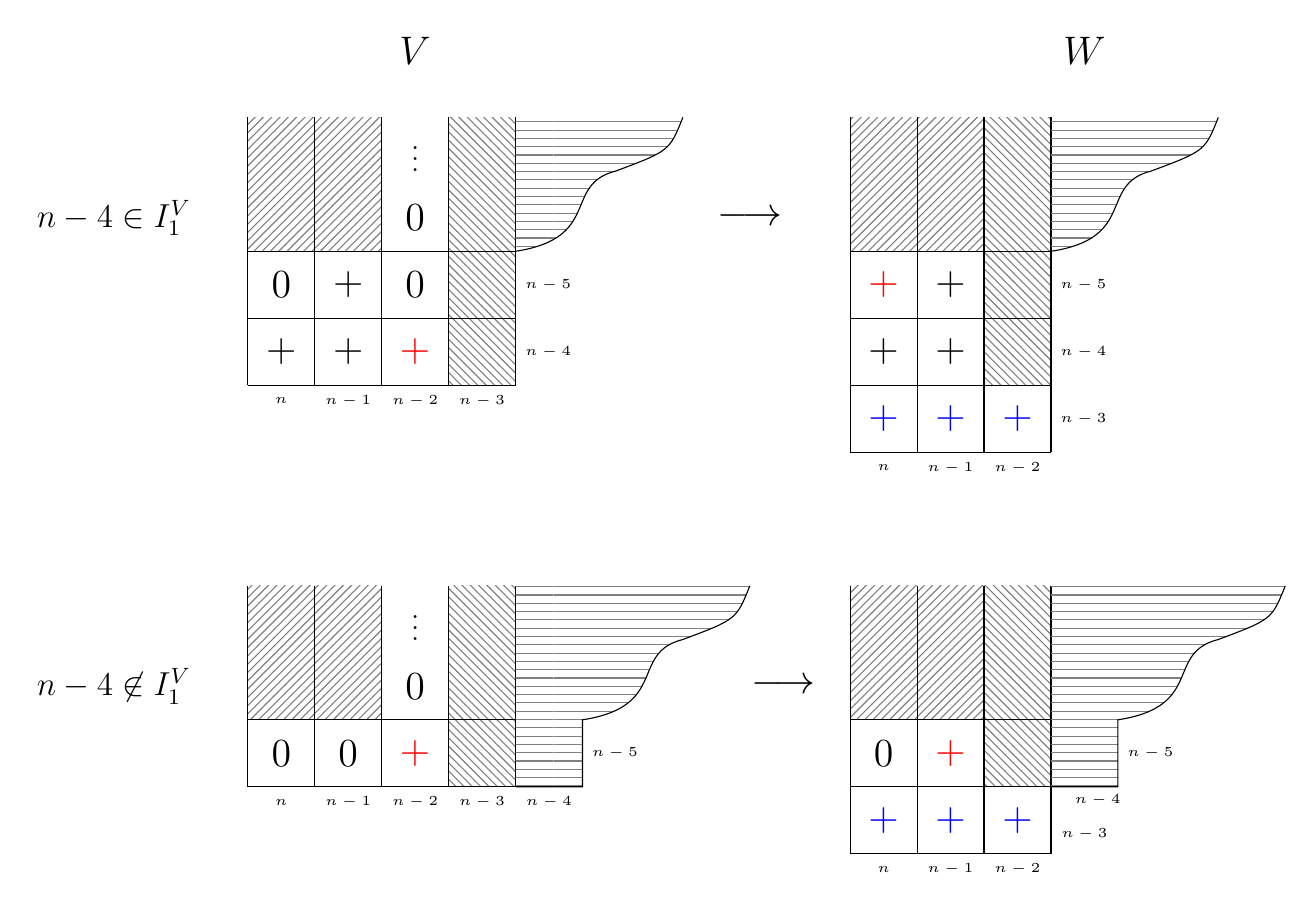
\begin{tikzpicture}[scale = 0.85]
\node at (2.5,5) {\Large $V$};
\node at (12.5,5) {\Large $W$};
\node at (-2,2.5) {\large $n-4 \in I_1^V$};
\node at (-2,-4.5) {\large $n-4 \not\in I_1^V$};
\node at (7.5,2.5) {\Large $\longrightarrow$};
\node at (8,-4.5) {\Large $\longrightarrow$};
% n-4 \in I_1, V
\begin{scope}
\draw[pattern color = gray,pattern = north east lines] (0,4) -- (0,2) -- (2,2) -- (2,4);
\draw[pattern color = gray,pattern = north west lines] (3,4) -- (3,0) -- (4,0) -- (4,4);
\draw (0,0) grid (4,2);
\foreach \x in {0,1,2,3,4} {
  \draw (\x,2) -- (\x,4);
  };
\foreach \c in {(0.5,0.5),(1.5,0.5),(1.5,1.5)} {
  \node at \c {\leplus};
}
\foreach \c in {(0.5,1.5),(2.5,1.5),(2.5,2.5)} {
  \node at \c {\lezero};
}
\node[red] at (2.5,0.5) {\leplus};
\node at (2.5,3.5) {$\vdots$};
\begin{scope}
\fill[pattern color = gray,pattern = horizontal lines] (4,2) .. controls (5.3,2.2) and (4.7,3) .. (5.5,3.2) .. controls (6.3,3.5) .. (6.5,4) -- (4,4) -- (4,2);
\draw (4,2) .. controls (5.3,2.2) and (4.7,3) .. (5.5,3.2) .. controls (6.3,3.5) .. (6.5,4);
\end{scope}
%\fill[color = white,path fading = south] (0,2) rectangle (6.5,4.1);
\node[below] at (0.5,0) {\tiny $n\vphantom{1}$};
\node[below] at (1.5,0) {\tiny $n-1$};
\node[below] at (2.5,0) {\tiny $n-2$};
\node[below] at (3.5,0) {\tiny $n-3$};
\node[right] at (4,0.5) {\tiny $n-4$};
\node[right] at (4,1.5) {\tiny $n-5$};
\end{scope}

% n-4 \in I_1, W
\begin{scope}[shift = {(9,0)}]
\draw[pattern color = gray,pattern = north east lines] (0,4) -- (0,2) -- (2,2) -- (2,4);
\draw[pattern color = gray,pattern = north west lines] (2,4) -- (2,0) -- (3,0) -- (3,4);
\draw (0,-1) grid (3,2);
\foreach \x in {0,1,2,3} {
  \draw (\x,2) -- (\x,4);
  };
\foreach \c in {(0.5,0.5),(1.5,0.5),(1.5,1.5)} {
  \node at \c {\leplus};
}
\node[red] at (0.5,1.5) {\leplus};
\foreach \c in {(0.5,-0.5),(1.5,-0.5),(2.5,-0.5)} {
  \node[blue] at \c {\leplus};
}
\begin{scope}[shift = {(-1,0)}]
\fill[pattern color = gray,pattern = horizontal lines] (4,2) .. controls (5.3,2.2) and (4.7,3) .. (5.5,3.2) .. controls (6.3,3.5) .. (6.5,4) -- (4,4) -- (4,2);
\draw (4,2) .. controls (5.3,2.2) and (4.7,3) .. (5.5,3.2) .. controls (6.3,3.5) .. (6.5,4);
\end{scope}
\node[below] at (0.5,-1) {\tiny $n\vphantom{1}$};
\node[below] at (1.5,-1) {\tiny $n-1$};
\node[below] at (2.5,-1) {\tiny $n-2$};
\node[right] at (3,-0.5) {\tiny $n-3$};
\node[right] at (3,0.5) {\tiny $n-4$};
\node[right] at (3,1.5) {\tiny $n-5$};
\end{scope}

% n-4 \not\in I_1, V
\begin{scope}[shift = {(0,-6)}]
\draw[pattern color = gray,pattern = north east lines] (0,3) -- (0,1) -- (2,1) -- (2,3);
\draw[pattern color = gray,pattern = north west lines] (3,3) -- (3,0) -- (4,0) -- (4,3);
\draw (0,0) grid (4,1);
\foreach \x in {0,1,2,3,4} {
  \draw (\x,1) -- (\x,3);
  };
\foreach \c in {(0.5,0.5),(1.5,0.5),(2.5,1.5)} {
  \node at \c {\lezero};
}
\node at (2.5,2.5) {$\vdots$};
\node[red] at (2.5,0.5) {\leplus};
\begin{scope}[shift = {(1,-1)}]
\fill[pattern color = gray,pattern = horizontal lines] (3,1) -- (4,1) -- (4,2) .. controls (5.3,2.2) and (4.7,3) .. (5.5,3.2) .. controls (6.3,3.5) .. (6.5,4) -- (3,4) -- (3,1);
\draw (3,1) -- (4,1) -- (4,2) .. controls (5.3,2.2) and (4.7,3) .. (5.5,3.2) .. controls (6.3,3.5) .. (6.5,4);
\end{scope}

\node[below] at (0.5,0) {\tiny $n\vphantom{1}$};
\node[below] at (1.5,0) {\tiny $n-1$};
\node[below] at (2.5,0) {\tiny $n-2$};
\node[below] at (3.5,0) {\tiny $n-3$};
\node[below] at (4.5,0) {\tiny $n-4$};
\node[right] at (5,0.5) {\tiny $n-5$};
\end{scope}

% n-4 \not\in I_1, W
\begin{scope}[shift = {(9,-6)}]
\draw[pattern color = gray,pattern = north east lines] (0,3) -- (0,1) -- (2,1) -- (2,3);
\draw[pattern color = gray,pattern = north west lines] (2,3) -- (2,0) -- (3,0) -- (3,3);
\draw (0,-1) grid (3,1);
\foreach \x in {0,1,2,3} {
  \draw (\x,1) -- (\x,3);
  };
\node at (0.5,0.5) {\lezero};
\node[red] at (1.5,0.5) {\leplus};
\foreach \c in {(0.5,-0.5),(1.5,-0.5),(2.5,-0.5)} {
  \node[blue] at \c {\leplus};
}
\begin{scope}[shift = {(0,-1)}]
\fill[pattern color = gray,pattern = horizontal lines] (3,1) -- (4,1) -- (4,2) .. controls (5.3,2.2) and (4.7,3) .. (5.5,3.2) .. controls (6.3,3.5) .. (6.5,4) -- (3,4) -- (3,1);
\draw (3,1) -- (4,1) -- (4,2) .. controls (5.3,2.2) and (4.7,3) .. (5.5,3.2) .. controls (6.3,3.5) .. (6.5,4);
\end{scope}
\node[below] at (0.5,-1) {\tiny $n\vphantom{1}$};
\node[below] at (1.5,-1) {\tiny $n-1$};
\node[below] at (2.5,-1) {\tiny $n-2$};
\node at (3.5,-0.7) {\tiny $n-3$};
\node at (3.7,-0.2) {\tiny $n-4$};
\node[right] at (4,0.5) {\tiny $n-5$};
\end{scope}
\end{tikzpicture}
\]
\caption{The Le diagrams for $V$ and $W$ in the setting of Theorem~\ref{thm dim}. The shaded regions indicate where the plusses match up perfectly, the red plusses exist if and only if $n-2 \in I_{n-2}^V$, and the blue plusses are the three new plusses coming from the induction step.}\label{fig:le diagrams bijection}
\end{figure}

\section{Poles of Wilson Loop Integrals}\label{sec poles} 

In this section we investigate the poles of the integrand for $I(W)$. Since SYM $N=4$ is a finite theory \cite{Alday:2007hr, ParkeTaylorids}, the scattering amplitudes (and thus the holomorphic Wilson loops $\,\mathfrak{W}_{k,n}$) are finite. That is, for a fixed set of external particles $\cZ$, we must have
\bas \sum_{W \text{ s.t. } |\cP| = k} I(W)(\cZ) <\infty \;.\eas
In other words, all poles of the intergrands must cancel. As a step towards this, in this section we prove some results about the structure of the denominator $R(W)$ of the integrand, as defined in Definition~\ref{def R(W)}.

The results of Section~\ref{sec GN algorithm} allow us to relate the configuration of propagators in a Wilson loop diagram $W$ to minors of $C(W)$, $R(W)$.  In this section fix an arbitrary ordering of the propagators, equivalently the rows of $C(W)$.\note{There's some grammatical issues in this paragraph and I'm not sure what it's supposed to be saying.}

The main result of this section is Theorem~\ref{thm denom}, which expresses the denominator $R(W)$ in terms of the Grassmann necklace of $W$. This simplifies the computation of $R(W)$ and allows us to directly relate the poles of the integral to the combinatorics of the diagram.

We first give an algorithm which extracts the required minors of $C(W)$ from the Grassmann necklace. 


\begin{algorithm}\label{alg WLD to denom via GN}
Let $W = (\cP,[n])$ be a Wilson loop diagram, and let $C(W)$ be the matrix of $W$ as defined in equation \eqref{C(W) dfn} with a fixed ordering on $\cP$ (see Section~\ref{section WLD background})\note{This was written before the exposition above; now I think we can simplify it to "Let $W$ be a WLD and $C(W)$ its associated matrix?}.
\begin{itemize}
  \item For each $i \in [n]$, we construct a factor $r_i$ as follows:
    \begin{itemize}
      %\item Use Algorithm~\ref{alg:put GN on WLD} to obtain a bijection between the propagators and the $i-1$st Grassmann necklace element, $I_{i-1}$.  (By convention set $I_{0}=I_n$.)  Write $I_{i-1}(p)$ for the vertex associated to propagator $p$ under this bijection.
      %\item Use Algorithm~\ref{alg:put GN on WLD} to obtain a bijection between the propagators and the $i$th Grassmann necklace element, $I_{i}$.  Write $I_{i}(p)$ for the vertex associated to propagator $p$ under this bijection.
      \item Let $S_i = \{p \in \cP \ | \ I_{i-1}(p) \neq I_i(p)\}$. (By convention, set $I_{0} = I_n$.)
	  %\item Write $\Delta_{I_i}$ for the determinant of the $k \times k$ minor of $C(W)$ with columns indexed by $I_i$.
      \item Let $r_i$ be the determinant of the $|S_i|\times |S_i|$ minor of $C(W)$ with rows indexed by $S_i$ and columns indexed by $I_i(S_i)$.  If $S_i = \emptyset$, set $r_i = 1$. %$\Delta_{I_i}$ with all variables from rows associated to $p\not\in S_i$ set to $1$.
    \end{itemize}
  \item Define $R = \prod_{i=1}^n r_i$.
\end{itemize}
\end{algorithm}

That is, each $r_i$ is the determinant of the minor determined by the propagators (rows) that contribute different values (columns) to the $i^{th}$ element of the Grassmann necklace than they did to the $i-1^{st}$. Since each $r_i$ is simply the determinant of a particular submatrix of $C(W)$ and an ordering on the propagators has been fixed, the sign of each $r_i$ is well-defined.

We also introduce the notation $\Delta_{I_i}$ to represent the determinant of the $k\times k$ minor of $C(W)$ with columns indexed by $I_i$. Note that one summand of this determinant is given by $\prod_{p \in \cP}x_{p, I_i(p)}$; the other summands are (up to sign) given by other bijections between the propagator set $\cP$ and the vertex set $I_i$.

Below, we show that the polynomial $R$ associated to Wilson loop diagram $W$ is equal to the denominator $R(W)$ from Definition~\ref{def R(W)}, and is the radical of the product $\prod_{i=1}^n \Delta_{I_i}$. First, however, we give a worked example of Algorithm~\ref{alg WLD to denom via GN}.

\begin{figure}
\begin{tabular}{rrrrr}
% \arrowangle is defined globally in the preamble for easy tweaking
\begin{tikzpicture}[rotate=67.5,baseline=(current bounding box.east)]
  \begin{scope}
  \drawWLD{7}{1.5}
  \drawnumbers
  \drawlabeledprop{1}{-1}{6}{0}{\footnotesize   $p$}
  \drawlabeledprop{1}{0}{5}{0}{\footnotesize   $q$}
  \drawlabeledprop{1}{1}{4}{0}{\footnotesize \; \qquad  $s$}
  \pgfmathsetmacro{\move}{\angle/\n};
  \draw[propassignment,red] (1.5*\angle + -1*\move:\radius) to[bend left = \arrowangle] (\angle*1:\radius); %p
  \draw[propassignment,red] (1.5*\angle:\radius) to[bend right = \arrowangle] (\angle*2:\radius); %q
  \draw[propassignment,red] (4.5*\angle:\radius) to[bend left = \arrowangle] (\angle*4:\radius); %r
  \node at (\angle*1.5:\radius*2) {$I_1$};
  \node[align = center] at (4*\angle:\radius*1.7) {$I_1(p) = 1, \; I_1(q) = 2,$ \\[5pt] $I_1(s) = 4$.};
    \end{scope}
  \end{tikzpicture} 
  & \quad \quad  &
\begin{tikzpicture}[rotate=67.5,baseline=(current bounding box.east)]
  \begin{scope}
  \drawWLD{7}{1.5}
  \drawnumbers
  \drawlabeledprop{1}{-1}{6}{0}{\footnotesize   $p$}
  \drawlabeledprop{1}{0}{5}{0}{\footnotesize   $q$}
  \drawlabeledprop{1}{1}{4}{0}{\footnotesize \; \qquad  $s$}
  \pgfmathsetmacro{\move}{\angle/\n};
  \draw[propassignment,red] (1.5*\angle + -1*\move:\radius) to[bend right = \arrowangle] (\angle*2:\radius); %p
  \draw[propassignment,red] (5.5*\angle:\radius) to[bend left = \arrowangle] (\angle*5:\radius); %q
  \draw[propassignment,red] (4.5*\angle:\radius) to[bend left = \arrowangle] (\angle*4:\radius); %r
  \node at (\angle*1.5:\radius*2) {$I_2$};
  \node[align = center] at (4*\angle:\radius*1.7) {$I_2(p) = 1,  \; I_2(s) = 4,$ \\[5pt] $I_2(q) = 5.$};
  \end{scope} 
\end{tikzpicture}
& \quad & 
\begin{tikzpicture}[rotate=67.5,baseline=(current bounding box.east)]
  \begin{scope}
  \drawWLD{7}{1.5}
  \drawnumbers
  \drawlabeledprop{1}{-1}{6}{0}{\footnotesize   $p$}
  \drawlabeledprop{1}{0}{5}{0}{\footnotesize   $q$}
  \drawlabeledprop{1}{1}{4}{0}{\footnotesize \; \qquad  $s$}
  \pgfmathsetmacro{\move}{\angle/\n};
  \draw[propassignment,red] (6.5*\angle:\radius) to[bend left = \arrowangle] (\angle*6:\radius); %p
  \draw[propassignment,red] (5.5*\angle:\radius) to[bend left = \arrowangle] (\angle*5:\radius); %q
  \draw[propassignment,red] (4.5*\angle:\radius) to[bend left = \arrowangle] (\angle*4:\radius); %r
  \node at (\angle*1.5:\radius*2) {$I_3 = I_4$};
  \node[align = center] at (4*\angle:\radius*1.7) {$I_3(s) = 4,\;  I_3(q) = 5,$ \\[5pt] $I_3(p) = 6.$ };
  \end{scope} 
\end{tikzpicture}  
\\ 
 & & & &  \\
 \begin{tikzpicture}[rotate=67.5,baseline=(current bounding box.east)]
  \begin{scope}
  \drawWLD{7}{1.5}
  \drawnumbers
  \drawlabeledprop{1}{-1}{6}{0}{\footnotesize   $p$}
  \drawlabeledprop{1}{0}{5}{0}{\footnotesize   $q$}
  \drawlabeledprop{1}{1}{4}{0}{\footnotesize \; \qquad  $s$}
  \pgfmathsetmacro{\move}{\angle/\n};
  \draw[propassignment,red] (6.5*\angle:\radius) to[bend right = \arrowangle] (\angle*7:\radius); %p
  \draw[propassignment,red] (5.5*\angle:\radius) to[bend right = \arrowangle] (\angle*6:\radius); %q
  \draw[propassignment,red] (4.5*\angle:\radius) to[bend right = \arrowangle] (\angle*5:\radius); %r
  \node at (\angle*1.5:\radius*2) {$I_5$};
  \node[align = center] at (4*\angle:\radius*1.7) {$I_5(s) = 5,\;  I_5(q) = 6,$  \\[5pt] $I_5(p) = 7$ };
  \end{scope} 
\end{tikzpicture}
& \quad & 
\begin{tikzpicture}[rotate=67.5,baseline=(current bounding box.east)]
  \begin{scope}
  \drawWLD{7}{1.5}
  \drawnumbers
  \drawlabeledprop{1}{-1}{6}{0}{\footnotesize   $p$}
  \drawlabeledprop{1}{0}{5}{0}{\footnotesize   $q$}
  \drawlabeledprop{1}{1}{4}{0}{\footnotesize \; \qquad  $s$}
  \pgfmathsetmacro{\move}{\angle/\n};
  \draw[propassignment,red] (6.5*\angle:\radius) to[bend right = \arrowangle] (\angle*7:\radius); %p
  \draw[propassignment,red] (5.5*\angle:\radius) to[bend right = \arrowangle] (\angle*6:\radius); %q
  \draw[propassignment,red] (1.5*\angle + 1*\move:\radius) to[bend left = \arrowangle] (\angle*1:\radius); %r
  \node at (\angle*1.5:\radius*2) {$I_6$};
  \node[align = center] at (4*\angle:\radius*1.7) {$I_6(q) = 6, \; I_6(p) = 7, $ \\[5pt] $I_6(s) = 1. $ };  
  \end{scope}
  \end{tikzpicture}  
& \quad &
\begin{tikzpicture}[rotate=67.5,baseline=(current bounding box.east)]
  \begin{scope}
  \drawWLD{7}{1.5}
  \drawnumbers
  \drawlabeledprop{1}{-1}{6}{0}{\footnotesize   $p$}
  \drawlabeledprop{1}{0}{5}{0}{\footnotesize   $q$}
  \drawlabeledprop{1}{1}{4}{0}{\footnotesize \; \qquad  $s$}
  \pgfmathsetmacro{\move}{\angle/\n};
  \draw[propassignment,red] (6.5*\angle:\radius) to[bend right = \arrowangle] (\angle*7:\radius); %p
  \draw[propassignment,red] (1.5*\angle:\radius) to[bend left = \arrowangle] (\angle*1:\radius); %q
  \draw[propassignment,red] (1.5*\angle + \move:\radius) to[bend right = \arrowangle] (\angle*2:\radius); %r
  \node at (\angle*1.5:\radius*2) {$I_7$};
  \node[align = center] at (4*\angle:\radius*1.7) {$I_7(p) = 1,  \; I_7(q) = 1, $ \\[5pt] $I_7(s) = 2.$};
  \end{scope} 
\end{tikzpicture}
\\
\end{tabular}
\caption{Example WLD for illustrating Algorithm~\ref{alg WLD to denom via GN} and bijections between propagators and vertices for each Grassmann necklace element.}\label{fig R eg}
\end{figure}

\begin{eg}
Consider the Wilson loop diagram in Figure~\ref{fig R eg}. Assigning propagators $p$, $q$, $r$ to rows $1,2,3$ respectively, we obtain the matrix
\[
C(W) = \begin{bmatrix} a & b & 0 & 0 & 0 & c & d \\ e & f & 0 & 0 & g & h & 0 \\ i & j & 0 & k & l & 0 & 0 \end{bmatrix}
\]
The Grassmann necklace of this diagram is 
\begin{gather*}I_1 = \{1,2,4\}, I_2 = \{2,4,5\}, I_3 = \{4,5,6\}, I_4=\{4,5,6\},\\ I_5=\{5,6,7\}, I_6 = \{6,7,1\}, I_7=\{7,1,2\}. \end{gather*}  
Figure~\ref{fig R eg} indicates indicates which vertex is contributed to $I_i$ by each propagator, for each $i \in [1,7]$.  

From $I_1$ to $I_2$, the propagators $p$ and $q$ change which vertices they contribute to; specifically, we have $I_1(p) = 1$ and $I_1(q)= 2$, while $I_2(p) = 2$ and $I_2(q)= 5$. On the other hand, $r$ contributes  4 to both $I_1$ and $I_2$. We therefore have $S_2 = \{p,q\}$.  The associated minors $\Delta_{I_2}$ and $r_2$ are therefore
\[
\Delta_{I_2}=\det\begin{bmatrix} b & 0 & 0 \\ f & 0 & g \\ j & k & l \end{bmatrix} = kgb, \qquad r_2 = \det\begin{bmatrix} b & 0 \\ f & g \end{bmatrix} = gb.
\] 
Continuing likewise, we get $r_3 = c$, $r_4=1$ (since $I_4 = I_3$), $r_5 = lhd$, and $r_6 = i$.

At $I_7$ we see for the first time an irreducible quadratic factor: we have $S_7 = \{q,s\}$ with ${I_7(S_7) = \{ 1,2\}}$, $\Delta_{I_7} = d(ej-fi)$ and $r_7 = ej-fi$. 

The irreducible quadratic factor corresponds to the fact that $q$ and $s$ share an edge {\em and} contribute both endpoints of that edge to $I_7$; see Proposition~\ref{prop alg gives rad} below.  

Finally, we have $r_1 = (af-be)k$.  Putting everything together, we obtain
\[
R = (af-be)kgbclhdi(ej-fi)
\]
which is squarefree and contains all factors of $\prod_{i=1}^{n}\Delta_{I_i}$. If one were to construct the denominator $R(W)$ associated to this Wilson loop diagram as per Definition~\ref{def R(W)}, we would find that we have $R(W) = R$.
\end{eg}

We are now ready to begin proving the main result of this section. We begin with a proposition stating several facts about $\Delta_{I_i}$ and their relationship to $r_i$.

\begin{prop}\label{prop alg gives rad}
  With notation as in Algorithm~\ref{alg WLD to denom via GN} we have the following:
  \begin{enumerate}
    \item Each $\Delta_{I_i}$ is homogeneous, as is each $r_i$.
    \item Each $\Delta_{I_i}$ splits into linear and quadratic factors.  All linear factors of  $\Delta_{I_i}$ are single variables and all irreducible quadratic factors are $2\times 2$ determinants of single variables.
    \item Quadratic factors in $\Delta_{I_i}$ arise precisely when propagators $p$ and $q$ are supported on a common edge \st{$(a,b)$}{\color{violet}$(a,a+1)$} with $I_i(p)=a$ and \st{$I_i(q)=b$}{\color{violet}$I_i(q)=a+1$}.\sanote{would like to make this change throughout}
    \item $r_i$ divides $\Delta_{I_i}$.
    \item The ideal generated by $R$ is the radical of the ideal generated by $\prod_{i=1}^{n}\Delta_{I_i}$.
  \end{enumerate}
\end{prop}

\begin{proof}
\begin{enumerate}
    \item The nonzero entries of $C(W)$ are independent indeterminates and so every $i\times i$ minor of $C(W)$ is either homogeneous of degree $i$ or is $0$.  Thus each $\Delta_{I_i}$ and each $r_i$ is homogeneous.  %Furthermore, each row contributes one factor to each term in the expansion of $\Delta_{I_i}$ so the result of setting the variables from a subset of rows to $1$ is still homogeneous.  Thus each $r_i$ is homogeneous.
    \item Viewing the determinant as a sum over permutations, and combining this with Corollary~\ref{lem basis as perm}, we see that $\Delta_{I_i}$ is a sum over bijections between $I_i$ and $\mathcal{P}$.  The nonzero terms in this sum are precisely those bijections such that each propagator is associated to one of its supporting vertices in $I_i$, namely \hlfix{$I_i(p)$}{do we mean $I_i(p)$ or $V(p)$ here? if the first, then the last part of the sentence is wrong}, since only those locations in $C(W)$ are nonzero.  Since the nonzero entries of $C(W)$ are independent there can be no cancellation between terms in this expansion. 

Suppose $\Delta_{I_i}$ has an irreducible factor $f$.  Let $\mathcal{P}'$ be the set of propagators which contribute a variable to $f$ and let $J$ be the set of vertices which contribute a variable to $f$.

The first claim is that the minor of $C(W)$ associated to $\mathcal{P}'$ and $J$ is precisely $f$.

{\em Proof of claim}: By the structure of determinants we know that $\Delta_{I_i} = fg$, where $g$ involves only variables associated to propagators not in $\mathcal{P}'$ and associated to vertices not in $J$.

Expanding out $fg$ yields a signed sum of monomials. Since there is no cancellation between terms, this means that the full expansion over permutations of $\Delta_{I_i}$ contains no other nonzero terms and hence no other variables.  Therefore $\Delta_{I_i}$ is equal to the determinant of the matrix obtained by taking the submatrix of $C(W)$ with columns indexed by $I_i$ and setting any variables not appearing in $\Delta_{I_i}$ to $0$.  This new matrix is, up to permutations of rows and columns, a block matrix with one block for $\mathcal{P}'$ and $J$ and the other block for the complements.  Thus its determinant, and hence also $\Delta_{I_i}$, is the product of the minors for these two blocks.  By considering which variables appear, these two factors must also be $f$ and $g$, and so in particular $f$ is the minor of $C(W)$ associated to $\mathcal{P}'$ and $J$.  This proves the claim.

A consequence of this claim is that every linear factor of $\Delta_{I_i}$ is a $1\times 1$ minor of $C(W)$, hence is a single variable, and every irreducible quadratic factor of $\Delta_{I_i}$ is a $2\times 2$ minor of $C(W)$, hence is a $2\times 2$ determinant of single variables.

All that remains is to prove that $\Delta_{I_i}$ has no irreducible factors of degree 3 or more.  Suppose for a contradiction that $f$ is a factor of $\Delta_{I_i}$ of degree $\geq 3$. Without loss of generality\footnote{This is without loss of generality for the following reason.  By removing the propagators which come before those contributing to $f$ (in the order given by $I_i$) and changing $i$ to be the first vertex which contributes to $f$, we obtain an admissible diagram.  In this diagram, $f$ still divides $\Delta_{I_i}$ and we also have $i\in I_i$ and that 
$i$ contributes to $f$.  Thus this diagram can be used in place of $W$.} we may assume $i\in I_i$ and that $i$ contributes to $f$.
Finally, we can suppose that $W$ is minimal in number of propagators with an irreducible factor of degree $\geq 3$. 

Let $p$ be the propagator such that $I_i(p) = i$. There are two cases to consider: when $p$ is supported on the edge $i-1$ or the edge $i$.  These are illustrated in Figure~\ref{fig no big factors}.




\begin{figure}
\[
\begin{tikzpicture}[baseline=(current bounding box.east),rotate=-20,scale = 0.95]
\begin{scope}
  \drawWLDfragment[8]{3}{0.4} 
  %\drawnumberspartial % use this to debug
  \newnode[left]{1}{i-1}
  \newnode[below]{2.5}{i}
  \newnode[below]{7}{m}
  \begin{scope}
    \clipcenterarc(0,0)(\startpoint-10:\endpoint+10:\radius)
    \newpropbend{1.9}{7.2}{60}
    \draw[smallpropagator,gray] (\zero+7.8*\step:\radius*1.1) to[bend left = 55] (\zero + 10*\step:\radius*1.1);
    \node at (\zero + 1.5*\step:\radius*0.5) {\footnotesize $p$};
  \end{scope}
  \node[align = center,black] at (\zero + \step*4.5:\radius*0.65) {\em \footnotesize propagators \\ \footnotesize \em inside $p$};
  \draw[propassignment,gray] (\zero + 1.81*\step:\radius) to[bend right = \arrowangle] (\zero + 2.5*\step:\radius); %p
  \draw[propassignment,gray] (\zero + 7.9*\step:\radius) to[bend left = \arrowangle] (\zero + 7*\step:\radius); 
  \node[align = center,black] at (\zero + 6.8*\step:1.5*\radius) {\em \footnotesize If $m \in I_i$ then it was \\ \em \footnotesize contributed by a propagator \\ \em \footnotesize outside of $p$};
  \node[align = center,black] at (110:\radius*0.5) {\em Case 1: $p = (i-1,m)$};
\end{scope}
\end{tikzpicture}
\qquad  
\begin{tikzpicture}[baseline=(current bounding box.east),rotate=-20,scale = 0.95]
  \begin{scope}
  \drawWLDfragment[8]{3}{0.4}  
  %\drawnumberspartial % use this to debug
  \newnode[left]{1}{i}
  \newnode[below]{2.5}{i+1\ \ \ }
  \newnode[below]{7}{j}
  \centerarc[red,line width = 2pt,line cap = round](0,0)(\zero + 1.61*\step:\zero+1.88*\step:\radius);
  \draw[propassignment,gray] (\zero + 1.55*\step:\radius) to[bend left = \arrowangle] (\zero + 1*\step:\radius); %p
  \draw[propassignment,gray] (\zero + 1.93*\step:\radius) to[bend right = \arrowangle] (\zero + 2.5*\step:\radius); %q 
  \draw[propassignment,gray] (\zero + 7.7*\step:\radius) to[bend left = \arrowangle] (\zero + 7*\step:\radius); % other prop
  \begin{scope}
    \clipcenterarc(0,0)(\startpoint-10:\endpoint+10:\radius)
    \newpropbend{1.9}{7.2}{40} % q
    \draw[smallpropagator] (\zero+1.6*\step:\radius*1.1) to[bend right = 40] (\zero  - 3*\step:\radius*1.1); % p
    \draw[smallpropagator,gray] (\zero+7.6*\step:\radius*1.1) to[bend left = 55] (\zero + 10*\step:\radius*1.1);
    \node at (\zero + 5*\step:\radius*0.32) {\footnotesize $q$};
    \node at (\zero + 1.1*\step:\radius*0.6) {\footnotesize $p$};
  \end{scope}
  \node[align = center,black] at (\zero + \step*4.5:\radius*0.72) {\em \footnotesize propagators \\ \footnotesize \em inside $q$};
  \node[align = center] at (\zero + 1.8*\step:\radius*1.5) {\footnotesize \em No \\ \footnotesize \em propagators \\ \footnotesize \em between \\ \footnotesize \em $p$ and $q$ \\ \footnotesize \em here};
  \node[align = center,black] at (\zero + 6.8*\step:1.5*\radius) {\em \footnotesize If $j \in I_i$ then it was \\ \em \footnotesize contributed by a propagator \\ \em \footnotesize outside of $q$};
    \node[align = center,black] at (110:\radius*0.5) {\em Case 2: $p = (i,j)$};

\end{scope}
\end{tikzpicture}
\]
  \caption{The two cases in the proof that no factors of $\Delta_{I_i}$ have degree 3 or more.}\label{fig no big factors}
\end{figure}





\textbf{Case 1}: Suppose $p = (i-1, m)$. Then $p$ has one end on the $i-1^{th}$ edge, and $I_{i+1}(p) = m$ by Remark~\ref{rmk cyclic}.

Let $S = \cP_{in}(p)$ be the set of propagators inside $p$ in the $<_i$ order.
By Remark \ref{rmk algorithm locally same}, $I_i$ and $I_{i+1}$ can only differ once $p$ contributes to $I_{i+1}$, so $I_i(q) = I_{i+1}(q)$ for each $q \in S \backslash \{p\}$. Thus if a propagator contributes $m$ in $I_i$ then it must lie outside $p$.


If neither $m$ nor $m+1$ appear in $I_i$ then by Corollary~\ref{no coloops} we have $V(p) \cap I_i = \{i\}$, and so the row of $p$ in the matrix of $\Delta_{I_i}$ has only one nonzero entry; hence $\Delta_{I_i}$ has a linear factor contributed by $p$ and $i$, which is a contradiction to the fact that $i$ contributes to $f$.  So we must have at least one of $m$ and $m+1$ in $I_i$. However, all propagators in $S$ contribute to $I_{i}$ strictly before $m$ by \st{the previous paragraph}{\color{violet}Remark {clockwise ordering rem}}\note{The purple edit isn't true: a priori a propagator inside $p$ could lie on edge $m$ and contribute $m$. The previous paragraph explains why this doesn't happen.} so, after permuting rows and columns as needed, the matrix giving $\Delta_{I_i}$ has the form
\[
\begin{bmatrix} A & B \\ 0 & C\end{bmatrix}
\]
where $A$ is the $|S|\times |S|$ matrix indexed by the propagators in $S$ and the vertices in $I_i(S)$. No other propagators can be supported on these vertices since all other propagators are outside of $p$, and $p$ is the first propagator supported at $i$; this explains the zero block.  Therefore $\Delta_{I_i} = \det A \det C$, and both factors are nontrivial since at least one of $m$ and $m+1$ appear in $I_i$.  Since $p\in \cP_{in}(p)$ we have $f|\det A${\color{violet}. If we remove the propagators that contribute variables to the minor $C$,}\st{ and if we remove the propagator outside of $p$ that contributes $m$ or $m+1$,} we get a diagram $W'$ with fewer propagators for which $\det A | \Delta_{I^{W'}_i}$ still holds, hence $f|\Delta_{I^{W'}_i}$.  This contradicts the minimality of our choices. \sanote{trying to make clear that the minor changes with the diagram. May have just made it too notation heavy.}

\textbf{Case 2}: Suppose $p = (i, m)$, i.e. $p$ has an end on the $i^{th}$ edge. If no other propagators are supported on the vertex $i$ then the corresponding column of $C(W)$ has only one nonzero entry in it, and so $\Delta_{I_i}$ has a linear factor contributed by $p$ and $i$; as above, this is a contradiction. \st{Since $I_i(p) = i$ there can be no propagator supported on $i$ with an end on the edge $(i-1, i)$.  Thus to have another propagator supported on $i$ there is at least one other propagator on edge $(i,i+1)$.  Further since since $I_i(p)=i$, one of these other propagators contributes $i+1$ in $I_i$, so we can take $q$ to be the propagator such that $I_i(q)=i+1$.  We know that $q$ has one end on the edge $(i, i+1)$ and is adjacent to $p$ on that edge in the counterclockwise direction (see Figure {\ref{fig no big factors}}).}  \hlfix{Since $p$ is the first propagator in the ordering imposed by $I_i$, it is the counterclockwise most propagator supported on $i$ (by Remark {\ref{clockwise ordering rem}}). Since there are multiple propagators supported on $i$, there must be a $q$ ending on edge $i$, such that $I_i(q) = i+1$, that is second clockwisemost propagators supported by $i$.}{Alt. proof} Write $q = (i, j)$ for the support of $q$.  The situation for $q$ is very similar to case 1: \st{in particular, we have $I_{i+1}(q) = j$ by Lemma {\ref{vertex cyclic int lem}} and so if $j\in I_i$ then the propagator which contributes $j$ is outside of $q$.}{\color{violet}if we have $r$ such that $I_i(r) = j$, as above, $r$ lies outside $q$: $r \in \cP_{out}(q, <_i)$. }

Similarly to Case 1, let $S = \cP_{in}(q) \cup \{p\}$ in the $<_i$ order. Then all propagators in $S$ contribute to $I_i$ strictly before $j$ and no other propagators are supported on vertices strictly before $j$.  Thus the matrix giving $\Delta_{I_i}$ has the form {\color{violet}(when reordered according to how they contribute to $I_i$)}
\[
\begin{bmatrix} A & B \\ 0 & C\end{bmatrix}
\]
where $A$ is the submatrix indexed by the propagators in $S$ and the vertices in $I_i(S)$. Again two things can now happen.  If some vertex $j$ or larger (with respect to $<_i$) belongs to $I_i$ then $B$ and $C$ are at least one column wide, and so the block form of the matrix gives a nontrivial factorization of $\Delta_{I_i}=\det A\det B$.  This yields a contradiction as in Case 1: $f|\det A$ and removing a propagator not in $S$ gives a smaller diagram with a factor of degree $\geq 3$, which contradicts our minimality assumption.\note{I rephrased this last sentence quite a bit because earlier things had gotten rephrased} \sanote{reads fine to me.}

On the other hand, if no vertex $\geq_i j$ is in $I_i$ then we have $\Delta_{I_i} = \det A$.  Looking in more detail into $A$, note that the only vertices that support both $p$ and $q$ and also belong to $I_i$ are $i$ and $i+1$. Hence
\[
A = \begin{bmatrix} D & 0 \\ E & F\end{bmatrix}
\]
where $D$ is the $2\times 2$ matrix indexed by the propagators $p$ and $q$ and the vertices $i$ and $i+1$.  Thus $p$ and $i$ contribute to a quadratic factor of $\Delta_{I_i}$, once again contradicting our assumptions.

All cases have now been covered and so $\Delta_{I_i}$ has only irreducible factors of degree $2$ or less.

\item \sanote{changed $b$ to $a+1$ here.} Suppose propagators $p$ and $q$ are supported on a common edge  $a$, with $I_i(p)=a$ and $I_i(q)=a+1$.  Let $x_{p,a},x_{p,a+1},x_{q,a},x_{q,a+1}$ be the associated variables in $C(W)$. For any fixed bijection $\sigma$ from $\cP\setminus\{p,q\}$ to $I_i \setminus\{a,a+1\}$ for which each propagator is supported on its image under the bijection, we can extend $\sigma$ to a bijection from propagators to $I_i$ in two ways: either $p\mapsto a$ and $q\mapsto a+1$ or $p\mapsto a+1$ and $q\mapsto a$.  The sum of the contributions of all these bijections to $\Delta_{I_i}$ is therefore the product of $x_{p,a}x_{q,a+1}-x_{p,a+1}x_{q,a}$ {\color{violet} By the arguments in the proof of the claim in part 2 of this theorem} \note{Could this use a ref back to where we discuss this kind of arugment in more detail.}\sanote{see violet?} with the minor coming from $\cP\setminus\{p, q\}$ and $I_i \setminus \{a,a+1\}$.  Since there is no cancellation of terms in the expansion of $\Delta_{I_i}$, if any other terms appear then they will cause a factor which is not in the form described in the previous part.  Therefore no such terms exist and $x_{p,a}x_{q,a+1}-x_{p,a+1}x_{q,a}$ is a factor of $\Delta_{I_i}$. 

Now let $f$ be a quadratic factor of $\Delta_{I_i}$.  By part (2) we know that $f$ is a $2\times 2$ minor coming from two propagators, call them $p$ and $q$, and two vertices, call them $a <_i b$.  It remains to show that \st{$a$ and $b$ are adjacent} {\color{violet}$b = a+1$}.  From this we can conclude that $p$ and $q$ each have one end on edge $a$. \st{, as any other way for both $p$ and $q$ to be supported on two consecutive vertices would contradict noncrossing or the density requirement of admissibility.}

As in the proof of part (2), make a new admissible diagram by removing the propagators which come before {\color{violet} those contibuting to} $f$ {\color{violet}in the order imposed by $I_i$} and set $i=a$. The cases in the proof of part (2) show how $\Delta_{I_i}$ factors: in particular the vertices supporting the other end of $p$ either do not appear in $I_i$, or they contribute to a different factor of $\Delta_{I_i}$ than $p$ and $a$ do.  By assumption $b$ contributes to the same factor as $a$.  Therefore $(a,b)$ is an edge defining an end of $p$, that is, $b = a+1$.

\item If $S_i = \emptyset$ then $r_i = 1$ and we immediately have $r_i | \Delta_{I_i}$; otherwise, let $p\in S_i$. Note that $\Delta_{I_i}$ is homogeneous linear in the variables of the row corresponding to $p$.  By part (2), either exactly one variable in the row corresponding to $p$ appears in $\Delta_{I_i}$ and this variable is a factor of $\Delta_{I_i}$, or exactly two variables from the row corresponding to $p$ appear in $\Delta_{I_i}$ and they appear as part of a quadratic factor.  In the first case let the variable be $x$. Then $x$ is a factor of $\Delta_{I_i}$. {\color{violet} Therefore, $x$ must correspond to entry in the row of $p$ and column of $I_i(p)$, i.e. $x = x_{p, I_i(p)}$.} \st{and so in particular the monomial in $\Delta_{I_i}$ corresponding to the bijection between propagators and vertices of $I_i$ associates the column of $x$ to $p$. Thus $x$ also appears in $r_i$ and s} Since the matrix for $r_i$ is a minor of the matrix for $\Delta_{I_i}$ \st{and every term in $\Delta_{I_i}$ involves $x$,} we also have that \st{every term in $r_i$ involves $x$ so}{\color{violet}$x$ is a factor of $r_i$.} \st{$x$ is a factor of both $r_i$ and $\Delta_{I_i}$ and is the only variable from this row in either polynomial.}

Now suppose two variables from the row $p$ appear in a quadratic factor $f$ of $\Delta_{I_i}$.  By part (3), there is another propagator $q$ and an edge $a$ such that $f$ is the $2\times 2$ minor coming from $p, q$ and $a, a+1$, with \st{$I_i(p)=a$, $I_i(q)=b$}.  {\color{violet}There are two situations which can occur, either $I_i(p)=a$ and $I_i(q)=a+1$, or $I_i(q)=a$ and $I_i(p)=a+1$. These are} illustrated in Figure~\ref{fig quadratic}; we show that in both cases it follows that $q \in S_i$ as well.

\begin{figure}
\[
\begin{tikzpicture}[baseline=(current bounding box.east)]
	\begin{scope}
	\drawWLDfragment[2]{4}{0.1} 
	%\drawnumberspartial % use this to debug
	\newnode[below]{1}{a}
	\newnode[below]{2}{a+1}
	\begin{scope}
	\clipcenterarc(0,0)(\zero - 1.5*\step:\zero + 4.5*\step:\radius)
	\newprop[midway,left]{1.33}{-7}{\footnotesize $p$}
	\newprop[midway,right]{1.66}{10}{\footnotesize $q$}
	\end{scope}
	\node at (\zero + 0.6*\step:\radius*0.7) {\footnotesize $p$};
	\node at (\zero + 2.4*\step:\radius*0.7) {\footnotesize $q$};
\end{scope}
\end{tikzpicture}
\begin{tikzpicture}[baseline=(current bounding box.east)]
	\begin{scope}
	\drawWLDfragment[2]{4}{0.1} 
	%\drawnumberspartial % use this to debug
	\newnode[below]{1}{a}
	\newnode[below]{2}{a+1}
	\begin{scope}
	\clipcenterarc(0,0)(\zero - 1.5*\step:\zero + 4.5*\step:\radius)
	\newprop[midway,left]{1.33}{-7}{\footnotesize $q$}
	\newprop[midway,right]{1.66}{10}{\footnotesize $p$}
	\end{scope}
	\node at (\zero + 0.6*\step:\radius*0.7) {\footnotesize $q$};
	\node at (\zero + 2.4*\step:\radius*0.7) {\footnotesize $p$};
\end{scope}
\end{tikzpicture}
\]
  \caption{The situations giving a quadratic factor with variables appearing in $r_i$. }\label{fig quadratic}
\end{figure}\note{I'm not sure we really need this figure? (Figure~\ref{fig quadratic})}

In both cases, since $I_{i-1}(p)\neq I_{i}(p)$ by assumption it follows from Lemma~\ref{vertex cyclic int lem} that $I_{i-1}(p) <_{i-1} I_{i}(p)$ and no other vertex supporting $p$ lies between $I_{i-1}(p)$ and $I_{i}(p)$. \st{In the case that $b<_i a$ and $q$ is assigned before $p$ in $I_i$,}{\color{violet} If $q$ lies clockwise of $p$, $I_i(q) = a$ and $q$ contributes before $p$ in $I_i$.} This means that $I_{i-1}(p)=a$ and so $I_{i-1}(q)\neq a$. Thus $q\in S_i$ and so $f$ is a factor of $r_i$.

Now consider the case where \st{$a<_i b$}{\color{violet}$I_i(q) = a+1$}, and suppose for contradiction that $q \not\in S_i$, i.e. that $I_{i-1}(q) = a+1$. Since $I_{i-1}(p) \neq a$, there must be some other propagator $s$ with $I_{i-1}(s) = a$ (else $q$ contributes $a$ to $I_{i-1}$). This propagator cannot lie on edge $a$, because then Remark~\ref{rmk cyclic} would imply that $I_i(s) \in \{a, a+1\}$, contradicting the fact that $I_i(p) = a$ and $I_i(q) = a+1$; thus $s$ has an end on edge $(a-1)$ and is inside $p$ in the $<_k$ order where $p=(k,a)$.

Say $s = (j,a-1)$ with $i-1 \leq_{i-1} k+1 \leq_{i-1} j+1$. But by Lemma~\ref{lem no fourth vertex}, if $I_{i-1}(s) = a$ then $a$ cannot be maximal in the support of $s$ with respect to $<_{i-1}$; thus we must have $i-1 = j+1$, and we are in the situation in Figure~\ref{fig part 4}.

\begin{figure}
\[
\begin{tikzpicture}[baseline=(current bounding box.east),rotate = -40]
	\begin{scope}
	\drawWLDfragment[8]{3}{0.4} 
	%\drawnumberspartial % use this to debug
	\newnode[left]{1}{j}
	\newnode[left]{2}{i-1}
	\newnode[below]{5}{a-1\quad}
	\newnode[below]{6}{a}
	\newnode[below]{7}{a+1}
	\begin{scope}
		\clipcenterarc(0,0)(\startpoint:\endpoint+\step:\radius)
		\newpropbend{1.5}{5.7}{20}
		\newpropbend{1.3}{6.4}{30}
		\newprop{6.6}{-6}{}
	\end{scope}
	\node at (\zero + 3.5*\step:\radius*0.8){\footnotesize $s$};
	\node at (\zero + 4.8*\step:\radius*0.45){\footnotesize $p$};
	\node at (\zero + 8*\step:\radius*0.65){\footnotesize $q$};
\end{scope}
\end{tikzpicture}
\]
  \caption{In order to obtain $I_{i-1}(s) = a$, propagators $s$ and $p$ must each have an end on edge $(i-2)$.}\label{fig part 4}
\end{figure}

Since $p$ changed its association from $I_{i-1}$ to $I_i$, we have $I_{i-1}(p) = i-1$ by Lemma~\ref{vertex cyclic int lem}. From Figure~\ref{fig part 4} {\color{violet} and Remark \ref{rmk algorithm locally same}}, $p$ contributes first to  $I_{i-1}$ and  then proceeds identically to $I_i$ for all vertices inside $p$ in the $<_{i-1}$ ordering, implying that $I_{i-1}(s) = I_i(s)$. Since $I_{i-1}(s) = a$ and $I_i(s) \neq a$, this is a contradiction. 

Thus $q\in S_i$ after all, and so $f$ is a factor of $r_i$ as required.

  

% Thus $s$ is supported on $a$ but does not have an edge on $(a,b)$ and so $s$ must have an end on $(a-1, a)$ and so be inside $p$ from the point of view of $i-1$.  Say $s$ is supported on $(j, j+1, a-1, a)$ and $p$ is supported on $(k, k+1, a, b)$ with $i-1 \leq_{i-1} k+1 \leq_{i-1} j+1$.  Again by Lemma~\ref{lem susama}, immediately after $s$ contributes $a$ it must contribute $j$ and so $I_i(s)=j$.

% Finally we want to show $I_i(s)=j$ gives a contradiction.  If $k=j$ then $I_{i}(s)= k$, but $p$ has not yet been taken as $I_i(p)=a$ and $p$ comes before $s$ around $k$, so this is a contradiction.  If $k+1=j$ then similarly $I_{i}(s)=k+1$ and yet $p$ comes before $s$ around $k$, a contradiction to $I_i(p)=a$.  Now suppose $k+1 <_{i-1} j$ then we have $i-1 \leq_{i-1} k+1 <_{i-1} I_i(s) = j$ so $i\leq_{i} I_i(s)$ which gives that
% \[
% I_i(s) <_i I_{i-1}(s) \qquad \text{and} \qquad I_i(s) <_{i-1} I_{i-1}(s)
% \]
% \note{Is this known to be impossible by the proof sketch of Lemma~\ref{lem susama} that you emailed or something similar.  I'm thinking this proof is already too long and the fact that this is impossible would be better as a lemma.}

\item If $W$ has zero propagators then all $I_i=\emptyset$ and both $R$ and $\prod_{i=1}^n \Delta_{I_i}$ are equal to $1$, so the result holds in this case.  Now assume $W$ has at least one propagator. \sanote{we never say this, but diagrams without propagators aren't really a thing.... at least they aren't tree level scatterings}

First we show that every factor of $\prod_{i=1}^n \Delta_{I_i}$ divides $R$.  Take an irreducible factor $f$ of $\prod_{i=1}^n \Delta_{I_i}$. There exists some $i$ such that $f|\Delta_{I_i}$ but $f\!\!\nmid\!\! \Delta_{I_{i-1}}$, since otherwise the variables corresponding to the propagators contributing to $f$ which do not themselves appear in $f$ could never appear, contradicting Lemma~\ref{vertex cyclic int lem}.  If $f$ is a linear factor, say from associating propagator $p$ to vertex $a$, then $I_{i}(p)=a$ and $I_{i-1}(p)\neq a$ so this factor appears in $r_i$.  If $f$ is a quadratic factor, \st{say from associating} {\color{violet} without loss of generality, associate} propagators $p$ and $q$ to vertices $a$ and $a+1$ respectively, then again we cannot have both $I_{i-1}(p) = a$ and $I_{i-1}(q) = a+1$, else $f$ divides $\Delta_{i-1}$. However, by the proof of part (4), if one of $p,q$ belongs to $S_i$ then the other does as well.  Thus $f$ divides $r_i$.

Next we need to show that $R$ is squarefree.  Suppose $f^2|R$.  If $f$ is a linear factor, say from associating propagator $p$ to vertex $a$, then there must be two distinct points in the Grassmann necklace algorithm where $p$ changes from not being associated to vertex $a$ to being associated to vertex $a$.  This contradicts Lemma~\ref{vertex cyclic int lem}.  Now suppose $f$ is a quadratic factor, say from propagators $p$ and $q$ supported on edge $a$ with $p$ clockwise to $q$ on the edge.  In this case it is not possible for any $I_i$ to associate $p$ to $a+1$ and $q$ to $a$.  Furthermore, we know by part (4) that $p$ changes from not being associated to $a$ to being associated to $a$ if and only if $q$ changes from not being associated to $a+1$ to being associated to $a+1$.  Thus $f^2|R$ implies that twice in the Grassmann necklace $p$ must change from not being associated to vertex $a$ to being associated to vertex $a$. This is again a contradiction, and so $R$ is squarefree.

Taking everything together we have that $R|\prod_{i=1}^n \Delta_{I_i}$, $R$ contains all factors of $\prod_{i=1}^n \Delta_{I_i}$ and $R$ is squarefree.  Therefore the ideal generated by $R$ is the radical of the ideal generated by $\prod_{i=1}^n \Delta_{I_i}$.
  \end{enumerate}
\end{proof}

We are now ready to prove the main theorem of this section. We use the facts about $\Delta_{I_i}$ and $R$ above to show that the denominator $R(W)$ of the integrand of $I(W)$ is given by Algorithm \ref{alg WLD to denom via GN}.

\begin{thm}\label{thm denom}
  Given any admissible Wilson loop diagram $W$, let $(I_1, \ldots I_n)$ be the associated Grasmann necklace. Then $R(W)$ as defined in Definition~\ref{def R(W)} is equal to the $R$ constructed by Algorithm~\ref{alg WLD to denom via GN}. Furthermore, the ideal generated by $R(W)$ is the radical of the ideal generated by $\prod_{i=1}^n \Delta_{I_i}$, where $\Delta_{I_i}$ is the determinant of the $k \times k$ minor indicated by $I_i$.  
\end{thm}

\begin{proof}
The equivalence of the ideal generated by $R$ and the radical of the ideal generated by $\prod_{i=1}^n \Delta_{I_i}$ is due to Proposition~\ref{prop alg gives rad}.  It remains to prove that $R(W)$ is the $R$ of Algorithm~\ref{alg WLD to denom via GN}.

To this end, first note that $R(W)$ and $R$ both have total degree $4|\mathcal{P}|$; the degree of $R(W)$ is immediate from the definition while that of $R$ \hlfix{follows from Lemma {\ref{vertex cyclic int lem}}}{one sentence explanation?}.  By Proposition~\ref{prop alg gives rad} every factor of $R$ is either a quadratic factor coming from two propagators supported on a common edge or a single variable coming from a support vertex of a propagator not appearing in a quadratic factor.  The factors of each $R_e$ making up $R(W)$ in the notation of Definition~\ref{def R(W)} are all of this form and every such factor occurs.  Hence every factor of $R$ divides $R(W)$.
Finally, since $R$ is squarefree, this implies that $R(W)$ is a scalar multiple of $R$.

Finally then we need to check the scalar.  By Definition~\ref{def R(W)} each linear factor appears with coefficient $1$ and each $2\times 2$ determinant factor appears with the same sign as the determinant of the corresponding minor in $C(W)$.  Therefore $R=R(W)$.
\end{proof}

Thus we have shown a deep relationship between the physically derived poles of the integrals $I(W)$ and the geometry and combinatorics associated to the diagrams $W$. At the very least, this is yet another piece of \hlfix{circumstantial}{can we find a better word for this?} evidence indicating that the positroid representation of Wilson loop diagrams is the correct geometric object to be considering when considering the Wilson loop amplitudes geometrically. 

While the authors cannot yet offer a proof that the appropriate sum of the Wilson loop diagrams are, in fact, finite, as expected from \cite{Alday:2007hr, ParkeTaylorids}, we do hope that this relationship to the Grassmann Necklace elements will provide a different avenue for answering that and related questions. \note{Can we rephrase this paragraph to be a bit more positive?}

\bibliographystyle{abbrv}
\bibliography{WLDbib}

% \begin{thebibliography}{10}
% \bibitem{Adamo:2011pv}
% Tim Adamo, Mathew Bullimore, Lionel Mason, and David Skinner.
% \newblock {Scattering Amplitudes and Wilson Loops in Twistor Space}.
% \newblock {\em J.Phys.A}, A44:454008, 2011.

% \bibitem{Adamo:2012xe}
% Tim Adamo and Lionel Mason.
% \newblock {Twistor-strings and gravity tree amplitudes}.
% \newblock {\em Class.Quant.Grav.}, 30:075020, 2013.

% \bibitem{wilsonloop}
% Susama Agarwala and Eloi~Marin Amat.
% \newblock Wilson loop diagrams and positroids.
% \newblock {\em Communications in Mathematical Physics}, 2016.
% \newblock arXiv:1509.06150.

% \bibitem{casestudy}
% Susama Agarwala and Sian Fryer.
% \newblock A study in $\textrm{Gr}_{\geq 0}(2,6)$: from the geometric case book
%   of {W}ilson loop diagrams and {SYM} $n=4$.
% \newblock arXiv:1803.00958.

% \bibitem{non-orientable}
% Susama Agarwala and Cameron Marcott.
% \newblock Wilson loops in sym $n=4$ do not parametrize an orientable space.
% \newblock arXiv:1807.05397.

% \bibitem{UnwindingAmplituhedron}
% Nima Arkani-Hamed, Hugh Thomas, and Jaroslav Trnka.
% \newblock Unwinding the amplituhedron in binary.
% \newblock {\em Journal of High Energy Physics}, 2018(1):16, Jan 2018.
% \newblock arXiv:1704.05069.

% \bibitem{Arkani-Hamed:2013kca}
% Nima Arkani-Hamed and Jaroslav Trnka.
% \newblock {Into the Amplituhedron}.
% \newblock {\em JHEP}, 12:182, 2014.

% \bibitem{Arkani-Hamed:2013jha}
% Nima Arkani-Hamed and Jaroslav Trnka.
% \newblock {The Amplituhedron}.
% \newblock {\em JHEP}, 10:30, 2014.

% \bibitem{Boels:2007qn}
% Rutger Boels, Lionel Mason, and David Skinner.
% \newblock {From twistor actions to MHV diagrams}.
% \newblock {\em Phys.Lett.}, B648:90--96, 2007.

% \bibitem{Bullimore:2010pj}
% Mathew Bullimore, Lionel Mason, and David Skinner.
% \newblock {MHV Diagrams in Momentum Twistor Space}.
% \newblock {\em JHEP}, 1012:032, 2010.

% \bibitem{CasteelsPaths}
% K. Casteels.
% \newblock Quantum matrices by paths.
% \newblock {\em Algebra Number Theory}, 8(8):1857--1912, 2014.

% \bibitem{Amplituhedronsquared}
% Burkhard Eden, Paul Heslop, and Lionel Mason.
% \newblock The AmplituhedronSquared.
% \newblock 2017.
% \newblock arxiv:1701.00453.

% \bibitem{galashinlam}
% P.~{Galashin} and T.~{Lam}.
% \newblock {Parity duality for the amplituhedron}.
% \newblock {\em arXiv e-prints}, May 2018.

% \bibitem{HeslopStewart}
% Paul Heslop and Alastair Stewart.
% \newblock The twistor wilson loop and the amplituhedron.
% \newblock {\em Journal of High Energy Physics}, 2018(10):142, Oct 2018.

% \bibitem{Hodges:2012ym}
% Andrew Hodges.
% \newblock {A simple formula for gravitational MHV amplitudes}.
% \newblock 2012.

% \bibitem{AmplituhedronDecomposition}
% Steven~N. Karp, Lauren~K. Williams, and Yan~X. Zhang.
% \newblock Decompostions of amplituhedra.
% \newblock arXiv:1708.09525.

% \bibitem{GrassmannAmplitudebook}
% Freddy Cachazo Alexander Goncharov Alexander Postnikov Jaroslav~Trnka
%   Nima~{A}rkani {H}amed, Jacob~Bourjaily.
% \newblock {\em Grassmannian Geometry of Scattering Amplitudes}.
% \newblock Cambridge University Press, Cambridge, UK, 2016.

% \bibitem{LipsteinMason}
% Arthur E. Lipstein, Lionel Mason
% \newblock From dlogs to dilogs; the super Yang-Mills MHV amplitude revisited
% \newblock J. High Energ. Phys. (2014) 2014: 169.

% \bibitem{reversingOh}
% S. Agarwala, S. Fryer.
% \newblock An algorithm to construct the Le diagram associated to a Grassmann necklace
% \newblock \url{arXiv:1803.01726}

% \bibitem{Gale}
% D. Gale.
% \newblock Optimal assignments in an ordered set: {A}n application of matroid theory.
% \newblock {\em J. Combinatorial Theory}, 4: 176 - 180 (1968).

% \bibitem{Oh}
% S. Oh.
% \newblock Positroids and {S}chubert matroids.
% \newblock {\em J. Combin. Theory Ser. A}, 118(8):2426--2435, (2011)

% \bibitem{Oh2}
%   S. Oh.
%   \newblock Combinatorics of positroids.
%   \newblock {\em DMTCS Proceedings vol. AK},(FPSAC 2009), 721--732

% \bibitem{Postnikov}
% A.~Postnikov.
% \newblock Total positivity, {G}rassmannians, and networks.
% \newblock \url{arXiv:math/0609764}.


% \end{thebibliography}

\end{document}
